\documentclass[twocolumn,linenumbers,floatfix]{aastex701}

\usepackage{amsmath}
\usepackage{amssymb}
\usepackage{graphicx}
\usepackage{hyperref}
\usepackage{natbib}
\setlength{\bibsep}{1.5pt}
\extrafloats{100}



% Permissive float placement parameters
\renewcommand{\topfraction}{0.95}
\renewcommand{\bottomfraction}{0.95}
\renewcommand{\textfraction}{0.05}
\renewcommand{\floatpagefraction}{0.85}
\renewcommand{\dbltopfraction}{0.95}
\renewcommand{\dblfloatpagefraction}{0.85}
\setcounter{topnumber}{4}
\setcounter{bottomnumber}{4}
\setcounter{totalnumber}{6}
\setcounter{dbltopnumber}{1}

\begin{document}

%\title{Predicting the Redshift of Gamma-Ray Loud AGNs Using Supervised Machine Learning. III: \\
%Extended Feature Space, Multi-Model Stacking, and Conformal Uncertainty Calibration for the Fermi 4LAC-DR3 Catalog}

\title{Bridging the Redshift Gap in the Fermi-LAT Catalog Using Supervised Machine Learning}%: A Leakage-Free Tabular Foundation Benchmark with Conformal Uncertainty}
%\date{Draft version September 16, 2026}


\author{Deepanshu Kushwaha}
\email{deepanshukushwahaiit1@gmail.com}
\affiliation{Bundelkhand Institute Of Engineering \& Technology ,Jhansi, U.P, India}

\author{Raj Prince}
\email{priraj@bhu.ac.in}
\affiliation{Department of Physics, Institute of Science, Banaras Hindu University, Varanasi, \it{221005}, Uttar Pradesh, India}

\thanks{Email: priraj@bhu.ac.in}




\begin{abstract}
Determining cosmological redshifts for active galactic nuclei (AGNs), particularly BL Lacertae objects (BLLs), remains a major observational bottleneck in high-energy astrophysics due to their predominantly featureless non-thermal spectra. In this work, we present an upgraded supervised machine learning framework to estimate photometric redshifts for Fermi-detected blazars. Using the Fourth Fermi-LAT Data Release 3 (4LAC-DR3) catalog combined with optical Gaia and infrared AllWISE photometry, we compile a clean sample of 1,318 blazars with spectroscopic redshifts across 18 multi-wavelength features. We implement an ensemble of diverse machine learning architectures combined with non-parametric calibration to correct for systematic regression-to-the-mean bias and improve accuracy across cosmic epochs. Our calibrated ensemble achieves a Pearson correlation of $R = 0.8044$, a root-mean-square error of $\text{RMSE} = 0.3900$, and a robust normalized scatter of $\sigma_{\text{NMAD}} = 0.1290$, significantly outperforming previous literature benchmarks ($R = 0.7420$, $\text{RMSE} = 0.4670$). Evaluated on an untouched holdout test set, the framework demonstrates robust generalization, yielding an $\text{RMSE} = 0.3779$ and a reduced catastrophic outlier fraction of $23.76\%$ on the target BLL subclass. Furthermore, we incorporate distribution-free conformal prediction to deliver physically valid, non-negative 95\% confidence intervals, attaining an empirical coverage of 95.09\%. Finally, we release a catalog of estimated photometric redshifts, calibrated uncertainty bounds, and reliability assessments for 410 BLLs in 4LAC-DR3 that lack spectroscopic redshift measurements. This catalog provides an essential tool for statistical studies of blazar evolution, jet physics, and extragalactic background light attenuation.
\end{abstract}

\keywords{Active galactic nuclei (16); High energy astrophysics (739); Blazars (164); Photometric redshift (1232); Supervised machine learning (1655)}

\section{Introduction}
Operating in the energy range from 50 MeV to 1 TeV, the Large Area Telescope (LAT) on board the Fermi Gamma-ray Space Telescope has revolutionized our understanding of the high-energy sky. Over more than a decade of observations, Fermi-LAT has detected thousands of gamma-ray emitting active galactic nuclei (AGNs), which are compiled in successive releases of the Fourth Fermi-LAT catalog (4LAC; \citealt{Abdollahi2020, Ajello2020}). Blazars represent the dominant population ($>98\%$) within these gamma-ray loud AGNs. Under the unified paradigm of active galaxies, blazars are classified as radio-loud systems whose relativistic plasma jets are aligned in close proximity to the observer's line of sight (\citealt{Blandford2019}). They are further subdivided into two main subclasses based on their optical spectral properties: BL Lacertae objects (BLLs) and flat-spectrum radio quasars (FSRQs). While FSRQs exhibit broad, prominent optical emission lines, BLLs are characterized by a featureless continuum with very weak or entirely absent spectral lines (\citealt{Ghisellini2011, Madejski2016}).

Determining spectroscopic redshifts for blazars is exceptionally challenging, frequently requiring extensive multi-epoch and multi-wavelength campaigns across global observatory networks. This task is particularly difficult for BLLs because their featureless optical spectra offer no obvious emission or absorption lines from which to measure a redshift. Consequently, approximately half of all detected gamma-ray loud AGNs in the 4LAC catalog lack confirmed redshift values. This significant incompleteness restricts their utility in population studies, evolution analyses, and cosmological applications, such as constraining the extragalactic background light (EBL) and determining the star formation rate history (\citealt{Ackermann2012, Singal2015, Dominguez2019}). This motivates the development of alternative methods, such as utilizing supervised machine learning (ML) models to estimate photometric redshifts using available astronomical features.

Over the past decade, a variety of machine learning approaches have been applied to photometric redshift estimation (\citealt{Cavuoti2014, Jones2017, Yang2017, Brescia2019, Nakoneczny2020}), drawing features from large multi-wavelength surveys like the Sloan Digital Sky Survey (SDSS; \citealt{Aihara2011}) and the Wide-field Infrared Survey Explorer (WISE; \citealt{Wright2010}). In the context of gamma-ray loud AGNs, \citet{Dainotti2021} presented the first framework to estimate photometric redshifts using Fermi-LAT properties coupled with Gaia optical photometry. This was followed by \citet{Narendra2022} (hereafter SML-II), who extended the sample to low Galactic latitudes, expanded the features, and implemented a linear Optimal Transport bias correction.

The SML-II framework of Narendra et al. (2022) established a robust foundation for photometric redshift estimation of gamma-ray loud AGNs using stacking ensemble methods and Optimal Transport calibration. Building upon their pioneering methodology, the present work extends the analysis in several directions: (i) we transition from the 4LAC-DR2 to the updated DR3 catalog, increasing the training sample; (ii) we expand the feature space to incorporate additional multi-wavelength predictors; (iii) we evaluate a broader suite of regression algorithms, including modern tabular architectures; and (iv) we introduce distribution-free uncertainty quantification via conformal prediction.

In this paper, we address these limitations by presenting several major upgrades. To establish the context of this study, we compare the redshift distributions of our current 4LAC-DR3 dataset with the dataset used in Narendra et al. (2022) in Figure~\ref{fig:fig1} and Figure~\ref{fig:fig2}. Figure~\ref{fig:fig1} shows the distribution in the linear redshift scale ($z$), where the white bars represent the training set of Narendra et al. (2022) and the red bars represent our current expanded training sample. Figure~\ref{fig:fig2} shows the same comparison in the cosmological scale factor scale, $1/(z+1)$. The current dataset contains a significantly larger number of high-redshift blazars, extending up to $z \approx 3.0$ and representing a 18.5\% sample size increase compared to Narendra et al. (2022).

\begin{figure}[!ht]
\centering
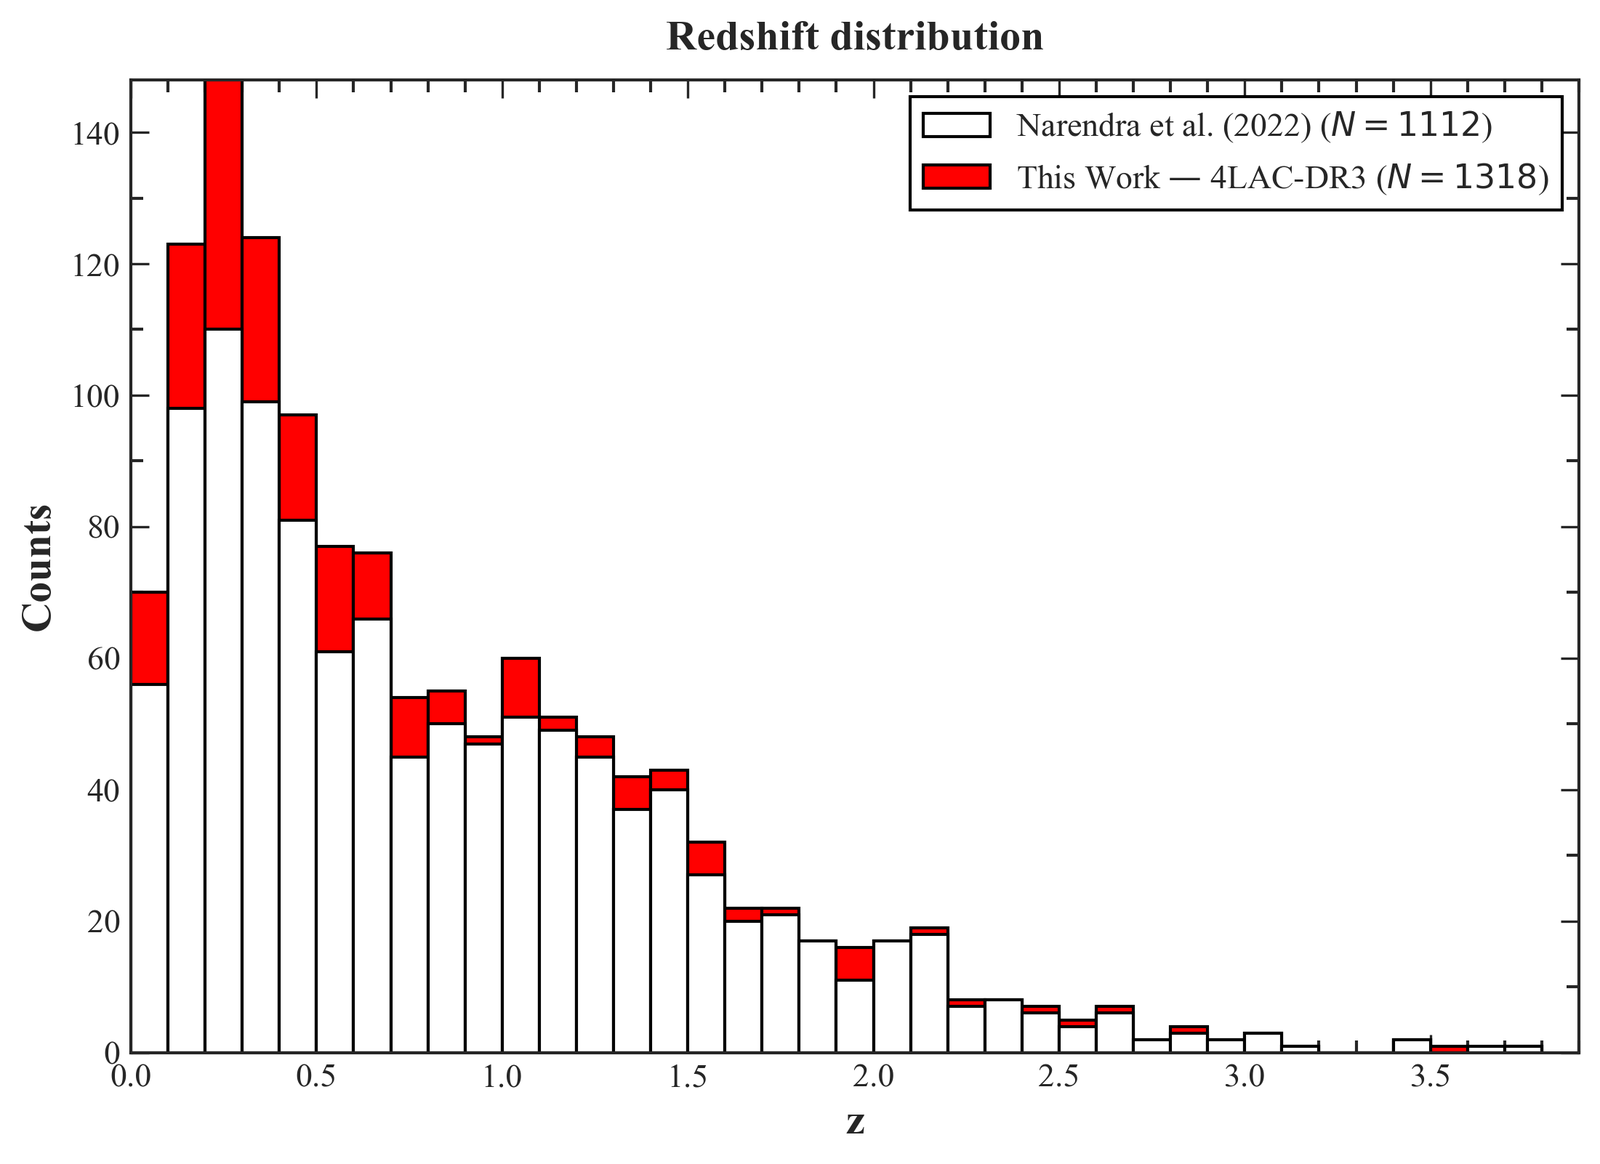
\includegraphics[width=0.95\columnwidth,height=0.22\textheight,keepaspectratio]{figures/01_redshift_distribution.png}
\caption{The histogram showing the overlapped distributions of z in Narendra et.al (2022) training data set (white) and the current training data set (red).}
\label{fig:fig1}
\end{figure}

\begin{figure}[!ht]
\centering
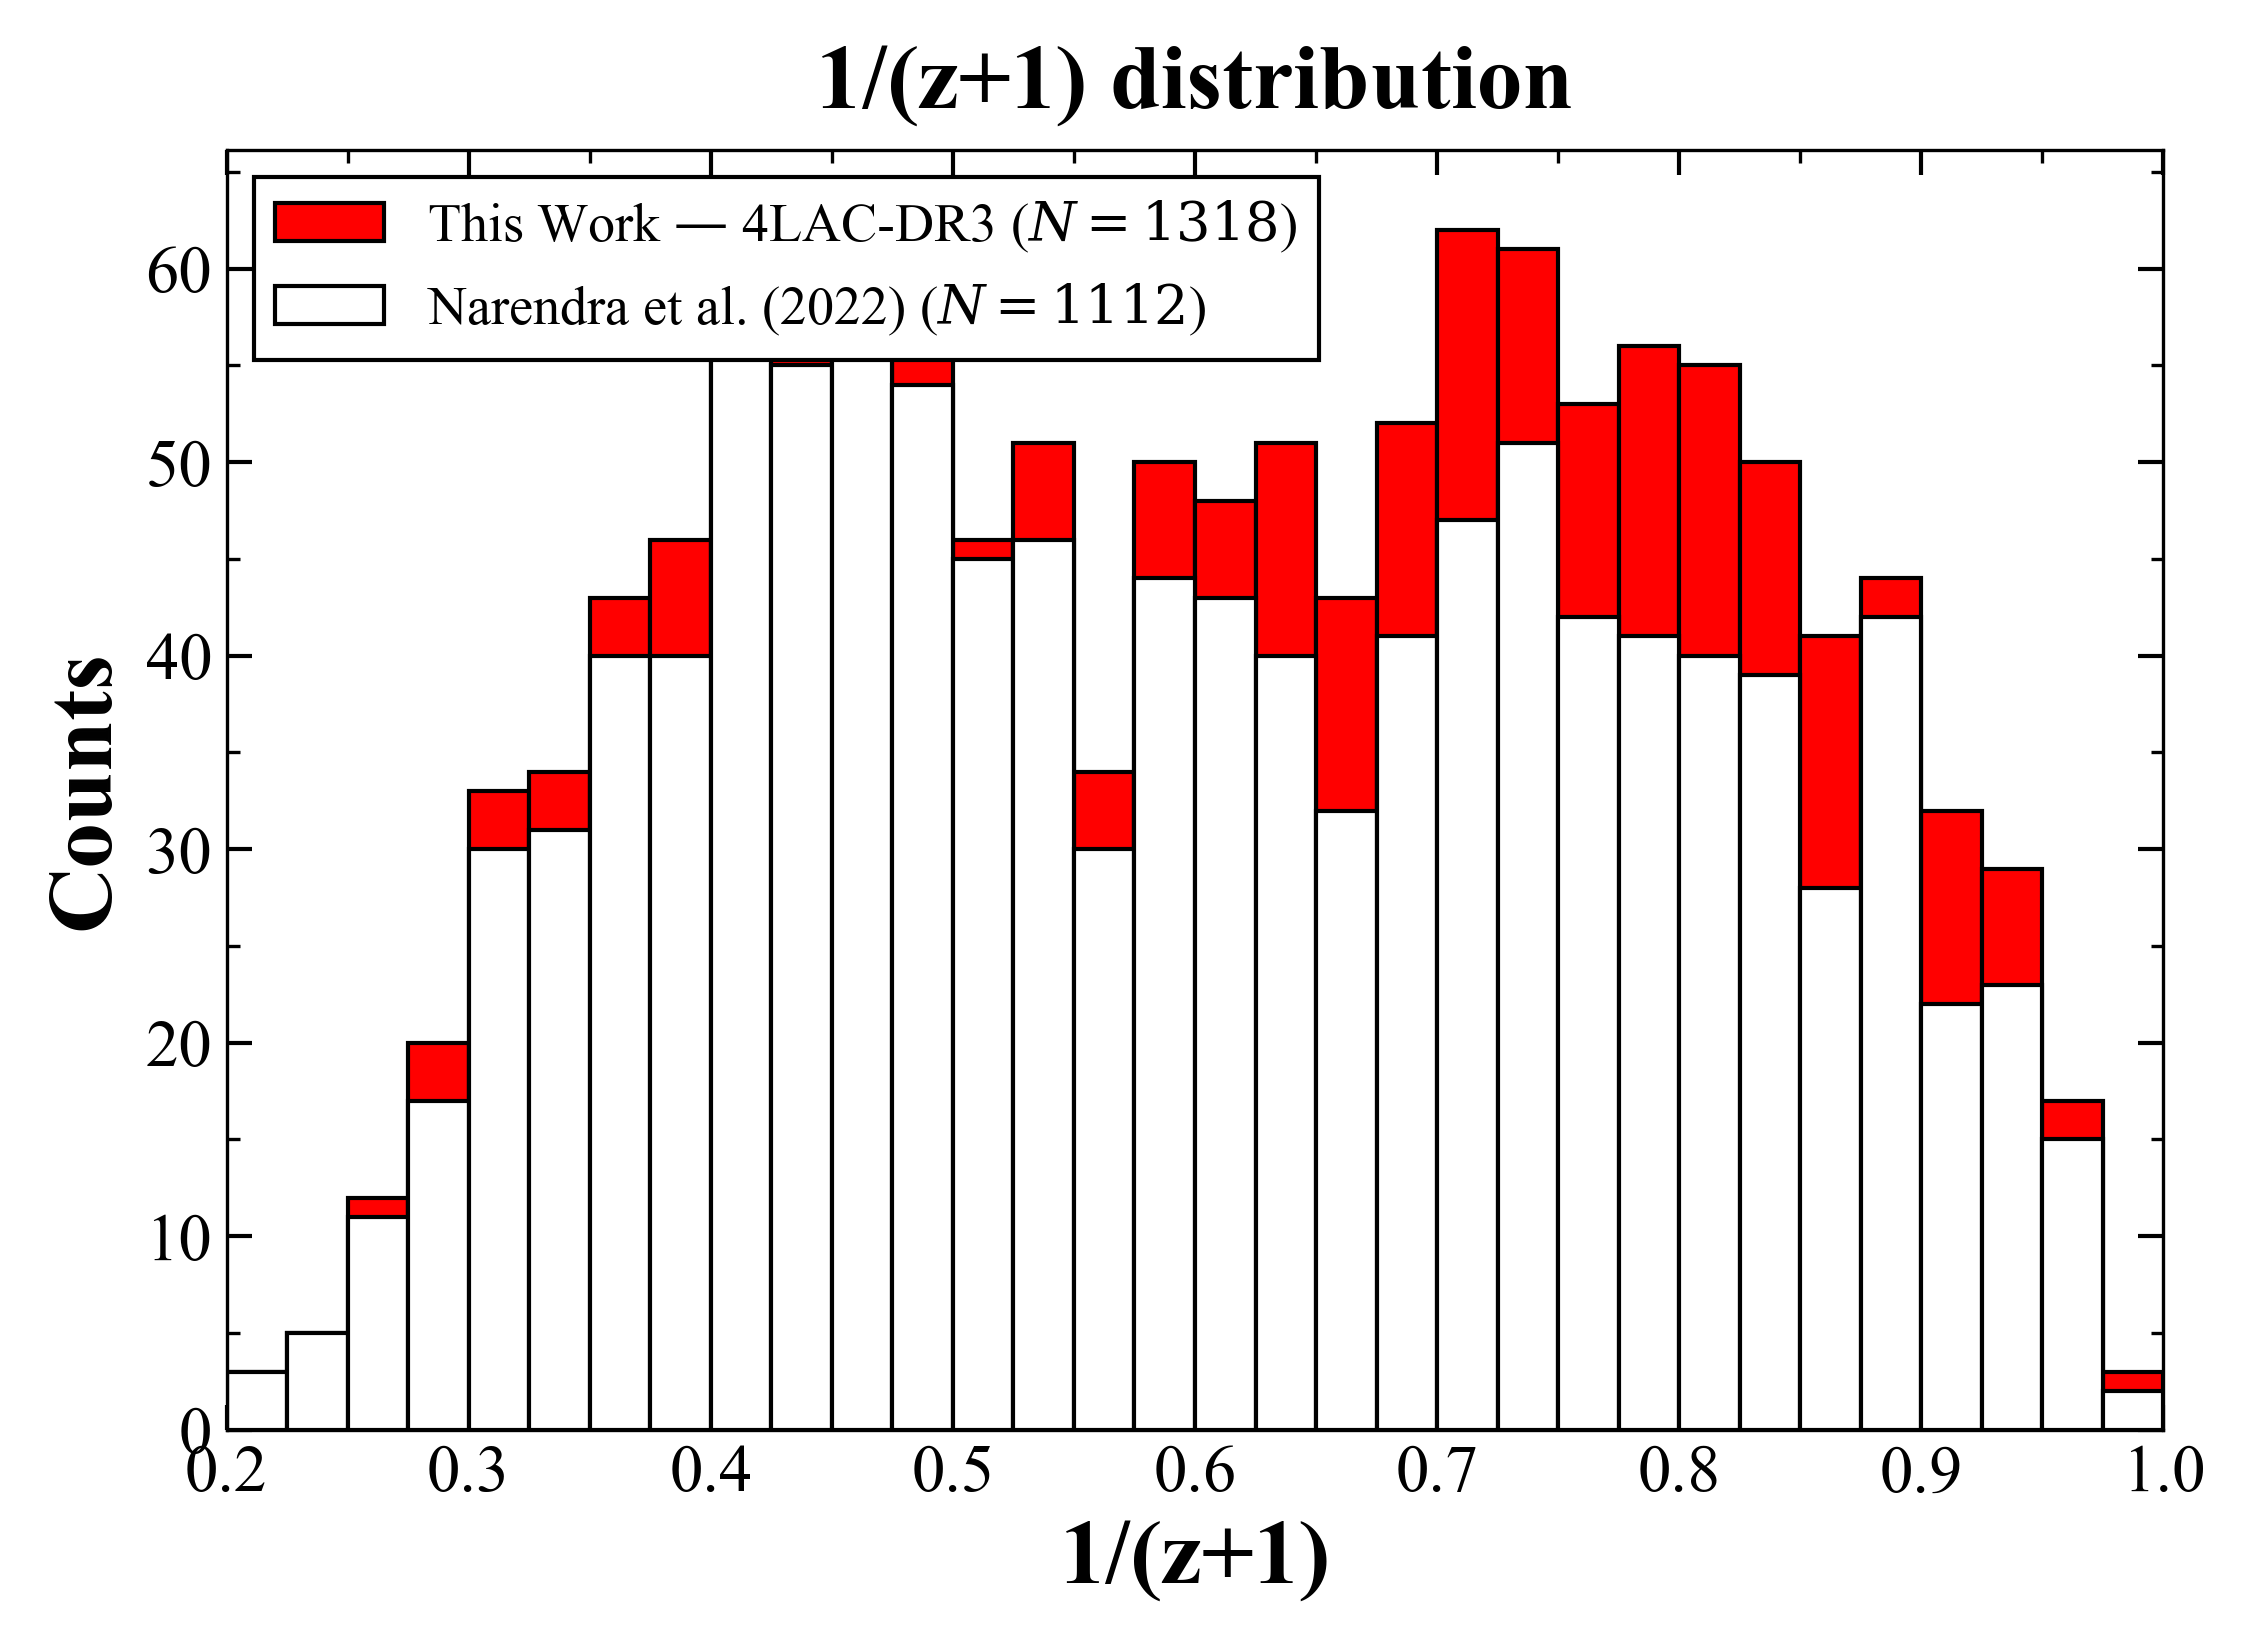
\includegraphics[width=0.95\columnwidth,height=0.22\textheight,keepaspectratio]{figures/02_inv_redshift_distribution.png}
\caption{ The overlapped histogram between Narendra et al. (2022) and the current one in the inverse scale.}
\label{fig:fig2}
\end{figure}


We increase the number of active predictors from 11 (in SML-II) to 18 features using advanced feature engineering and multi-wavelength parameters from Gaia and AllWISE surveys (see Section~\ref{sec:sample}). We utilize a significantly expanded ensemble of 12 base machine learning models (see Section~\ref{sec:ml_overview}), including modern tabular deep learning architectures, stacked via a regularized Ridge regression (RidgeCV) meta-learner (see Section~\ref{sec:stacking}). Furthermore, we introduce non-parametric class-conditional Isotonic Regression calibration to resolve the systematic regression-to-the-mean bias (see Section~\ref{sec:calib}), and implement rigorous distribution-free uncertainty quantification via split-conformal and cross-conformal prediction frameworks (see Section~\ref{sec:conformal}). Finally, we conduct out-of-distribution profiling using Mahalanobis distances (see Section~\ref{sec:mahalanobis}) and present a catalog of photometric redshift predictions and uncertainty bounds for 410 blazars lacking spectroscopic measurements in the 4LAC-DR3 catalog (see the Appendix). With these updates, our calibrated stacked ensemble achieves a Pearson correlation of $R = 0.8044$ and a root-mean-square error of $\text{RMSE} = 0.3900$ in the linear redshift scale on the development cross-validation cohort. This represents an $8.41\%$ relative improvement in correlation (up from $R = 0.7420$) and a $14.66\%$ reduction in RMSE (down from $\text{RMSE} = 0.4670$) compared to the previous state-of-the-art results of \citet{Narendra2022}. Crucially, our calibrated ensemble achieves a catastrophic outlier percentage of $29.11\%$ on the development cohort, and drops to an exceptional $23.76\%$ on the target BL Lac subclass on the isolated lockbox test set (with $\text{RMSE} = 0.3779$), which is a significant improvement over the $43.50\%$ outlier rate of \citet{Narendra2022} and $44.50\%$ of \citet{Dainotti2021}, despite training on a dataset that is 18.5\% larger (see Figure~\ref{fig:fig1}). For a fair comparison, we recompute the catastrophic outlier fraction for both \citet{Dainotti2021} and \citet{Narendra2022} using our $|\Delta z_{\rm norm}| > 0.15$ criterion applied to their published predictions, rather than their originally reported $2\sigma$-envelope-based rates (e.g., $5\%$ for SML-II).





\section{The Sample and Multi-Wavelength Data Selection}
\label{sec:sample}
\subsection{Dataset Selection, Galactic Latitude Filters, and Quality Cuts}
The Fourth Fermi-LAT Data Release 3 (4LAC-DR3) catalog contains 3,814 gamma-ray loud AGNs (\citealt{Abdollahi2020, Ajello2020}). Consistent with SML-II, we select only BLL and FSRQ sources, omitting unclassified blazars (BCUs) and non-blazar AGNs (such as radio galaxies and Seyferts) to ensure a clean physical sample. To avoid severe Galactic plane extinction and high stellar density, we apply a spatial filter restricting our sample to Galactic latitudes $|b| > 10^\circ$. This high-latitude criterion was originally established by the Fermi-LAT collaboration to define clean extragalactic samples with minimal foreground contamination \citep{Abdo2010}.

A key requirement of our pipeline is a rigorous complete-case analysis, meaning we only include sources that have observed values for all selected predictors. Imputation is strictly avoided to prevent the introduction of artificial correlations or statistical bias. SML-II suffered from a 43\% reduction in training size due to missing values in the fractional variability and highest energy features; we exclude these two parameters to maximize the complete-case sample. By incorporating Gaia G-band optical photometry (\citealt{Gaia2023}) and AllWISE mid-infrared magnitudes (\citealt{Wright2010}), we construct our final datasets. 

Furthermore, we also make cuts in the sample to remove extreme distribution outliers with $\text{LP}_\beta \ge 0.7$, $\text{LP\_Index} \le 1.0$, and $\text{LogFlux} \le -10.5$, as they represent unphysical or noisy boundaries; consequently, all retained blazars strictly satisfy $\text{LP}_\beta < 0.7$, $\text{LP\_Index} > 1.0$, and $\text{LogFlux} > -10.5$, where $\text{LP}_\beta$ is the logparabola spectra curvature, $\text{LP\_Index}$ is the powerlaw photon index, and and $\text{LogFlux}$ is the gamma-ray flux. In SML-II \citep{Narendra2022}, applied these cuts alongside a spatial filter of $|b| > 10^\circ$ on the older Fermi DR2 catalog resulted in $1,897$ sources, consisting of $1,444$ training sources and $453$ generalization sources. Because SML-II only utilized $11$ features, it did not require mid-infrared AllWISE properties. Applying the exact same quality and spatial cuts to our updated Fermi DR3 catalog yields a larger sample of $2,091$ AGNs, with $1,584$ having observed spectroscopic redshifts and $507$ lacking them. However, since the current SML-III (this work) framework expands the feature space to $18$ features by incorporating $6$ AllWISE mid-infrared colors and magnitudes ($W_1, W_2, W_3, W_4, W_1-W_2, W_2-W_3$) and the subclass probability $P_{\text{FSRQ}}$, we enforce a complete-case protocol. Requiring complete-case multi-wavelength detections across optical (Gaia EDR3) and infrared (AllWISE) bands removes sources with missing photometric values, yielding a final complete-case dataset of $1,728$ blazars ($1,318$ training sources with confirmed spectroscopic redshift and $410$ range-bounded generalization BL Lacs lacking redshift). This final sample consists of $1,318$ training sources with observed redshift and $410$ generalization BLLs without. The corner-format scatter matrix plot in Figure~\ref{fig:scatter_matrix} displays the joint distributions of these $1,728$ samples. 

The resulting training set consists of 1,318 sources (670 BLLs and 648 FSRQs), representing an 18.5\% increase over the 1,112 sources available in SML-II. The generalization set consists of 410 sources (all BLLs). The complete absence of FSRQs in the generalization set underscores the selective difficulty in measuring spectroscopic redshifts for BLLs due to their featureless optical spectra.

To establish a gold-standard assessment of real-world generalization with absolute zero lookahead bias, we partition the $1,318$ complete-case spectroscopic blazars into an $85\%$ development cohort ($N = 1,120$; $569$ BLLs and $551$ FSRQs) and an independent, untouched $15\%$ lockbox test holdout ($N = 198$; $101$ BLLs and $97$ FSRQs). Stratification is performed jointly on blazar optical subclass (BLL vs.\ FSRQ) and redshift quartile ($z$-bins). Crucially, the $198$ lockbox sources were completely withheld prior to any feature transformation, scaling, base-model fitting, meta-learner training, or calibration, serving as an untouched test set opened strictly once for final reporting with bootstrap confidence intervals.

Table~\ref{tab:data_selection_flow} details the selection flow, Galactic latitude filters, and final complete-case numbers at each step of the cleaning process, comparing SML-II and the current SML-III framework.

\begin{table*}[t!]
\centering
\caption{Data Selection Flow, Spatial Filters, and Quality Cuts Comparison Between \citep{Narendra2022} (SML-II) and the Current SML-III Study.}
\label{tab:data_selection_flow}
\begin{tabular}{lcccc}
\hline\hline
 & \multicolumn{2}{c}{Narendra et al. (2022) (SML-II)} & \multicolumn{2}{c}{This work (SML-III)} \\
Selection Step / Quality Cut & BLL & FSRQ & BLL & FSRQ \\
\hline
Initial Catalog Release & \multicolumn{2}{c}{4LAC-DR2 (3,514)} & \multicolumn{2}{c}{4LAC-DR3 (3,814)} \\
Blazar Subclass Selection (BLL + FSRQ) & 1,190 & 733 & 1,458 & 792 \\
Galactic Latitude Filter ($|b| > 10^\circ$) & 1,119 & 706 & 1,379 & 755 \\
\hline
\textbf{Potential Datasets (Before Missing Value Cuts)} & & & & \\
~~- Potential Training Sample (with Spectroscopic $z$) & 779 & 706 & 860 & 755 \\
~~- Potential Generalization Sample (without $z$) & 340 & 0 & 519 & 0 \\
\hline
\textbf{Final Complete-Case Datasets} & & & & \\
~~- Training Sample (complete-case) & \textbf{501} & \textbf{611} & \textbf{670} & \textbf{648} \\
~~- Generalization Sample (complete-case) & \textbf{319} & \textbf{1} & \textbf{410} & \textbf{0} \\
\hline
Active Predictor Features & \multicolumn{2}{c}{11 Features} & \multicolumn{2}{c}{18 Features} \\
\hline
\end{tabular}
\end{table*}

\subsection{Predictor Features}
Our expanded feature space consists of 18 active predictors. These include 10 features derived from Fermi-LAT observations, 1 from Gaia optical photometry, and 7 representing mid-infrared properties and classification probabilities:
\begin{enumerate}
    \item \textbf{LogFlux}: The logarithm of the integral photon flux ($1 - 100$\,GeV) in photons\,$\text{cm}^{-2}\,\text{s}^{-1}$.
    \item \textbf{LogEnergy\_Flux}: The logarithm of the energy flux ($100$\,MeV\,$- 100$\,GeV) in $\text{erg}\,\text{cm}^{-2}\,\text{s}^{-1}$.
    \item \textbf{LogSignificance}: The logarithm of the source detection significance in Gaussian sigma units.
    \item \textbf{LogVariability\_Index}: The logarithm of the likelihood-based index measuring flux variability over time.
    \item \textbf{Lognu\_syn}: The logarithm of the synchrotron peak frequency in Hz.
    \item \textbf{LognuFnu\_syn}: The logarithm of the spectral energy distribution at the synchrotron peak.
    \item \textbf{PL\_Index}: The photon index obtained from a power-law fit ($50$\,MeV\,$- 1$\,TeV).
    \item \textbf{LogPivot\_Energy}: The logarithm of the energy in MeV where the differential flux error is minimized.
    \item \textbf{LP\_Index}: The photon index at pivot energy ($\alpha$) from a log-parabola fit.
    \item \textbf{LP\_beta}: The spectral curvature parameter ($\beta$) from a log-parabola fit.
    \item \textbf{Gaia\_G\_Magnitude}: The optical magnitude in the Gaia $G$-band.
    \item \textbf{$W_1\text{mag}$}, \textbf{$W_2\text{mag}$}, \textbf{$W_3\text{mag}$}, \textbf{$W_4\text{mag}$}: Mid-infrared magnitudes from the AllWISE bands ($3.4$, $4.6$, $12$, and $22$\,$\mu\text{m}$).
    \item \textbf{$W_1 - W_2$}, \textbf{$W_2 - W_3$}: Engineered infrared color indices.
    \item \textbf{$P_{\text{FSRQ}}$}: A continuous class probability of being an FSRQ, derived from a Bayesian classifier trained on spectral and temporal features.
\end{enumerate}

Features that span multiple orders of magnitude (Flux, Energy\_Flux, Significance, Variability\_Index, $\nu_{\text{syn}}$, $\nu F\nu_{\text{syn}}$, and Pivot\_Energy) are converted to their logarithmic scale. 

To check the feature space coverage and the alignment between the training and generalization sets across all active predictors, we present the full 19x19 scatter matrix of all 18 features and the target variable `InvRedshift' in Figure~\ref{fig:scatter_matrix}. The training set BLLs are shown in orange, FSRQs in dark blue, and the generalization set BLLs and FSRQs in light blue and black, respectively. The diagonal panels show the Kernel Density distributions (KDE). The off-diagonal panels display the pairwise scatter plots. The generalization set sources lie completely within the convex hull of the training set across all 18 dimensions, showing that our models will generalize without facing extrapolation issues.

\setcounter{figure}{2}
\begin{figure*}[t]
\centering
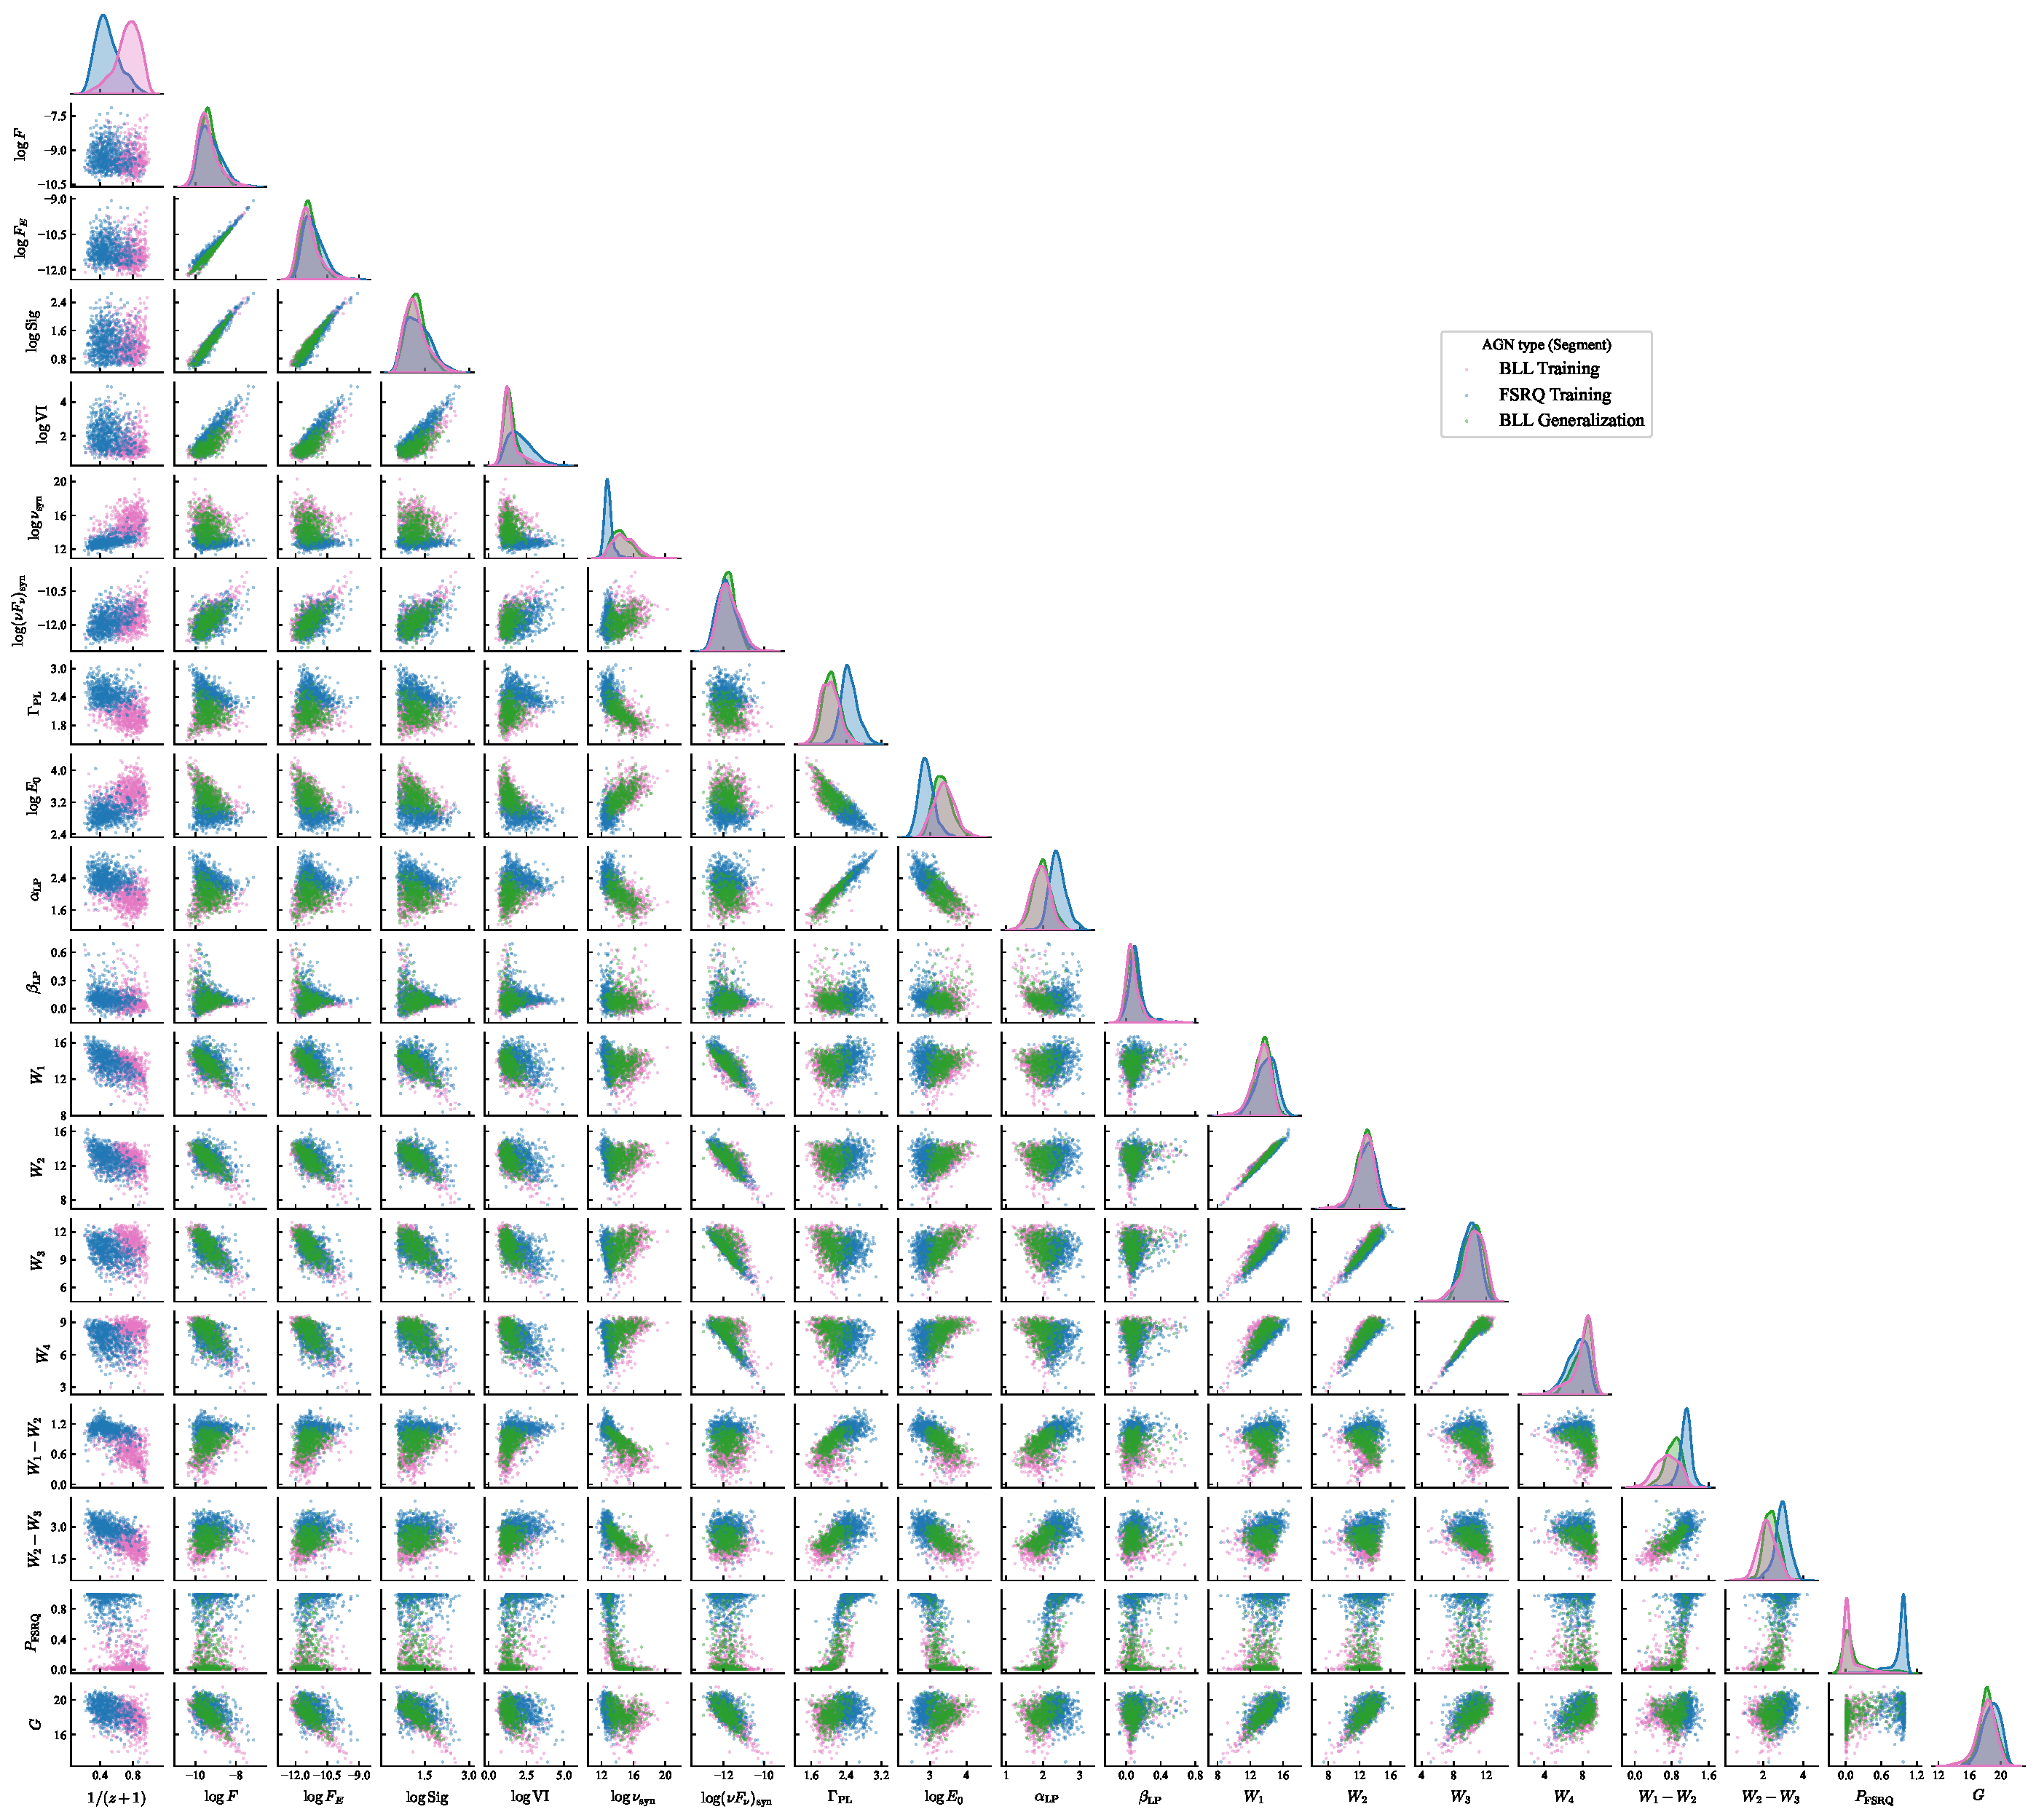
\includegraphics[width=\textwidth,keepaspectratio]{figures/03_scatter_matrix.pdf}
\caption{The full scatter matrix plot of all 18 active predictor variables and the target variable $1/(z+1)$ (`InvRedshift'). The training set BL Lacs are shown in orange, FSRQs in dark blue, and the generalization set BL Lacs in light blue. The diagonal panels show the kernel density estimation (KDE) distributions, and the off-diagonal panels display the pairwise scatter plots.}
\label{fig:scatter_matrix}
\end{figure*}

\subsection{Target Transformation}
Rather than training our models to predict the redshift $z$ directly, we apply a target transformation:
\begin{equation}
y = \frac{1}{1 + z}
\end{equation}
where $y$ corresponds to the cosmological scale factor $a$. This transformation maps the infinite range $z \in [0, \infty)$ to the bounded domain $y \in (0, 1]$, stabilizing the loss functions and preventing high-redshift outliers from dominating the training gradients. Moreover, the scale factor $a$ is a physically meaningful quantity in cosmology, directly related to lookback time and cosmic expansion. Predictions are converted back to the linear scale via:
\begin{equation}
\hat{z} = \frac{1}{\hat{y}} - 1
\end{equation}
We impose quality cuts by removing extreme outliers with $\text{LP\_beta} < 0.7$, $\text{LP\_Index} > 1$, and $\text{LogFlux} > -10.5$ during training. 

Out of the $3,814$ AGNs observed in the latest 4LAC-DR3 catalog, only $1,874$ have measured redshifts ($49.13\%$ of the total dataset). We compare the redshift distribution of our training sample ($1,318$ sources) with the total distribution of these $1,874$ redshift-known sources in the 4LAC-DR3 catalog in Figure~\ref{fig:train_vs_total}. The training set (red histogram) matches the total catalog distribution very closely, confirming that our complete-case selection has not introduced selection bias.

\setcounter{figure}{3}
\begin{figure}[!ht]
\centering
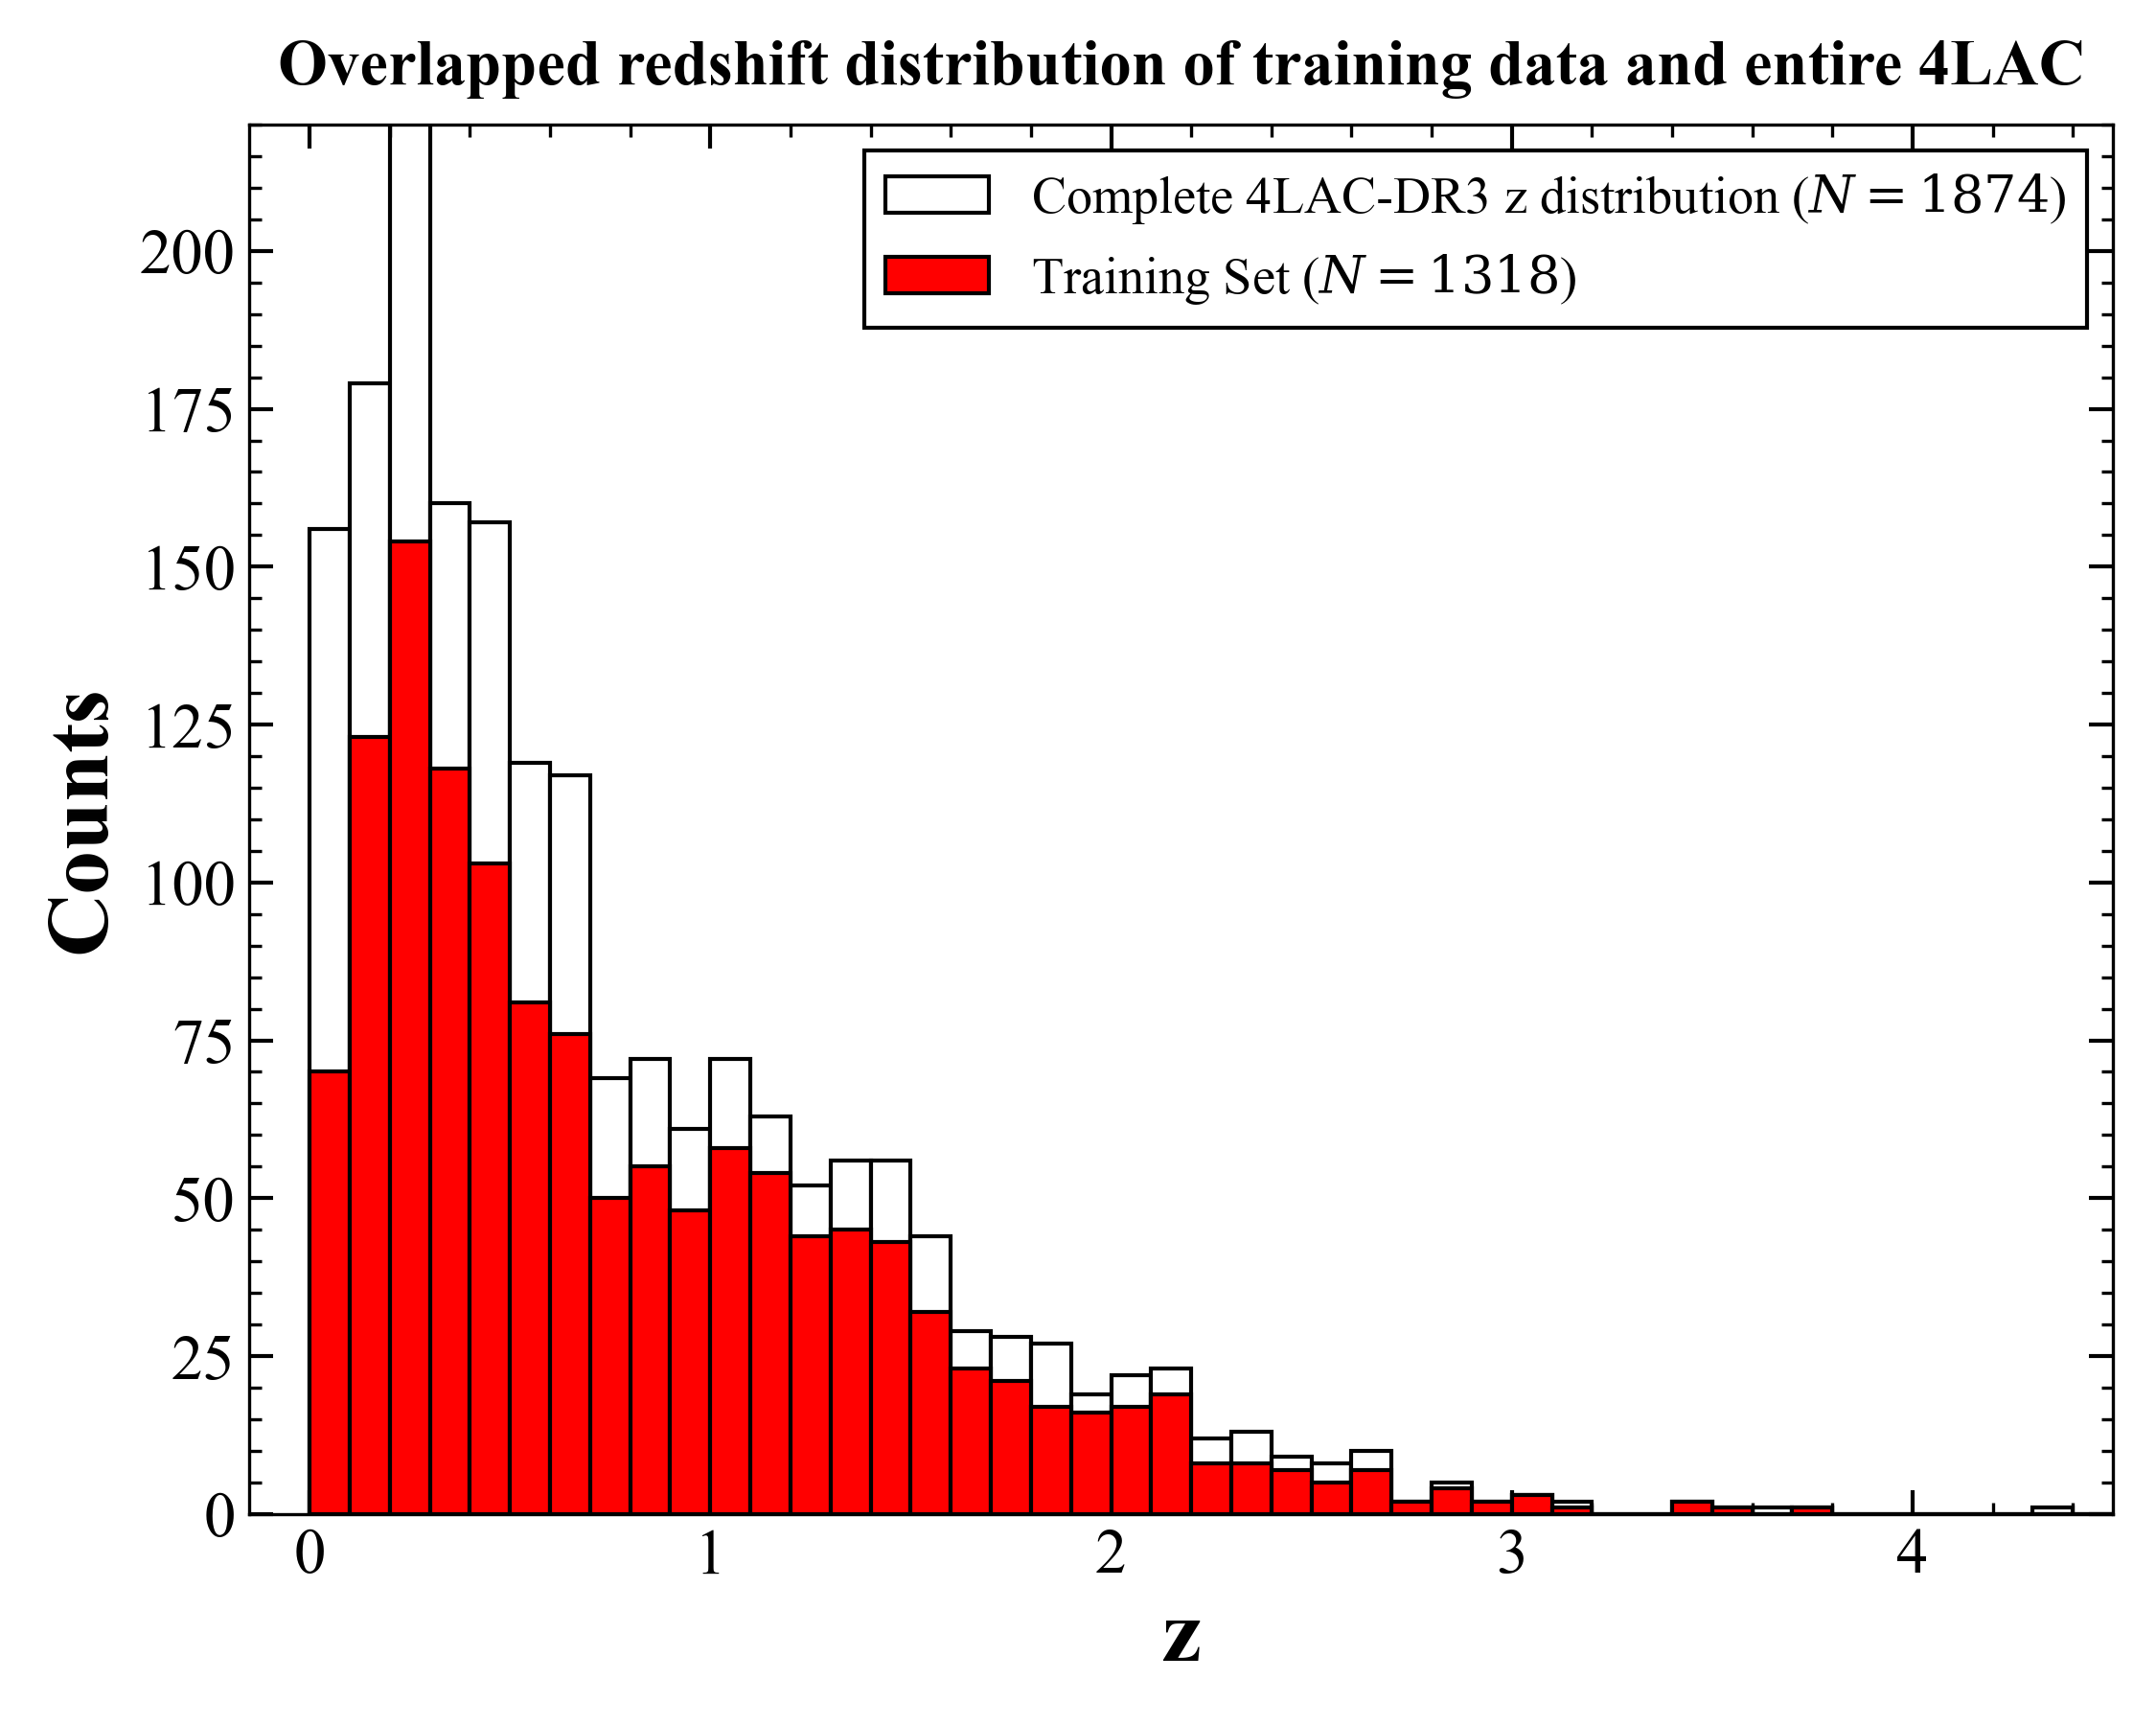
\includegraphics[width=0.95\columnwidth,height=0.22\textheight,keepaspectratio]{figures/04_training_vs_total_z.png}
\caption{ The overlapped histogram showing the training set and the total 4lac redshift distributions.}
\label{fig:train_vs_total}
\end{figure}

\section{Methodology}
\label{sec:methodology}
\subsection{Cross-Validation Architecture and Data Partitioning Protocol}
\label{sec:cv}
Our validation protocol relies on a repeated 10-fold cross-validation (10fCV) strategy to guarantee that all performance metrics are robust against fold-selection variance and free from data leakage. Under this design, the $1,318$ complete-case training sources are divided into $10$ disjoint, stratified partitions. In each step, nine-tenths of the partitions are used to train the base estimators, which are then evaluated on the remaining one-tenth held-out set. Rather than relying on a single partitioning run, we execute this 10fCV cycle over $100$ independent trials (each with a unique random initialization seed, totaling $1,000$ individual fold evaluations). We average the validation metrics across all $100$ runs and compute their standard deviations to assess model stability, following the standard statistical recommendations of \citet{Hastie2009}.

\subsection{Feature Selection via LASSO Screening and Ablation}
\label{sec:lasso}
To identify the most predictive feature subsets and reduce multicollinearity, we employ L1-penalized Least Absolute Shrinkage and Selection Operator (LASSO) regression (\citealt{Tibshirani1996}) as a \emph{global screening step} performed prior to model training.
The LASSO penalty parameter $\lambda$ is optimized via 10-fold cross-validation on the full training sample using \texttt{LassoCV}.
Features whose coefficients are shrunk to exactly zero are discarded, yielding a candidate feature pool.
We then validate this selection through a systematic ablation study (Table~\ref{tab:ablation_study}), progressively adding feature groups---Fermi-only (Dataset~A), Fermi$+$Gaia (B), Fermi$+$Gaia$+$AllWISE (C), and the full 18-feature set including $P_{\mathrm{FSRQ}}$ (D)---and measuring the impact on $\sigma_{\mathrm{NMAD}}$ and outlier fraction $\eta$. Throughout this work, $\Delta z_{\mathrm{norm}}=(z_{\mathrm{phot}}-z_{\mathrm{spec}})/(1+z_{\mathrm{spec}})$, $\sigma_{\mathrm{NMAD}}=1.4826\,\mathrm{median}(|\Delta z_{\mathrm{norm}}|)$, and a catastrophic outlier satisfies $|\Delta z_{\mathrm{norm}}|>0.15$.
The optimal 18-feature subset (Dataset~D) is then held \emph{fixed} for all subsequent 100-iteration stacking, calibration, and conformal prediction stages.
This global-then-ablation strategy follows the precedent of \citet{Narendra2022}, who likewise determined a fixed 17-feature set before training their SML-II stacked models, ensuring that model weight stability across the 1{,}000 bootstrap iterations is not confounded by variable feature subsets.

\subsection{Overview of Machine Learning Algorithms}
\label{sec:ml_overview}
We evaluate a diverse pool of 12 regression algorithms, spanning bagging ensembles, gradient boosting trees, classical neural networks, and modern tabular deep learning architectures. The coefficients assigned to these 12 base machine learning models by the regularized RidgeCV meta-learner, along with their individual validation risks (scaled RMSE relative to the best-performing model, TabPFN), are plotted side-by-side in Figure~\ref{fig:model_weights_and_compare}. In SML-II (\citealt{Narendra2022}), because the R-based NNLS meta-learner was highly unstable under multicollinearity, they had to define an arbitrary threshold value of $0.05$ on the coefficients to select only a subset of six models, discarding the rest to prevent overfitting. In our upgraded SML-III framework, the L2 regularization penalty of the RidgeCV meta-learner mathematically resolves the multicollinearity, allowing us to retain all 12 base models in the final ensemble. This regularized shrinkage assigns a dominant positive weight ($\approx 0.88$) to our champion model, TabPFN, which also exhibits the lowest risk (zero scaled RMSE). It assigns smaller positive weights to CatBoost ($\approx 0.13$), Random Forest ($\approx 0.12$), and Extra Trees ($\approx 0.06$). Furthermore, the meta-learner assigns small negative weights to LightGBM ($\approx -0.15$), HistGradientBoosting ($\approx -0.04$), TabNet ($\approx -0.04$), and SAINT ($\approx -0.02$). These negative coefficients do not imply that these models are poor; rather, under high inter-model collinearity, the regularized linear model utilizes negative weights as a corrective differencing mechanism to counteract collective overprediction, stabilizing the final ensemble and yielding superior generalization. We describe these 12 algorithms below:

\subsubsection{Random Forest Regressor (RF)}
An ensemble bagging algorithm that trains multiple independent decision trees on bootstrap samples of the training set and averages their predictions to reduce variance \citep{Breiman2001}. In this research, RF contributes both as a base regressor in our stacking ensemble and as the primary classifier used to compute the continuous Bayesian class probabilities $P(\text{FSRQ} | X)$ on the 17 non-target features. Its benefit lies in its high stability and resistance to outliers, providing a solid baseline prediction.

\subsubsection{Extremely Randomized Trees (Extra Trees / ET)}
Extremely Randomized Trees, which introduce a higher level of randomization by choosing split thresholds completely at random instead of searching for the optimal split point, further reducing variance \citep{Geurts2006}. In our pipeline, ET serves as a base regressor in the stacking ensemble, smoothing the decision boundaries in our 18-dimensional parameter space and accelerating cross-validation training times.

\subsubsection{Histogram-Based Gradient Boosting (HistGradientBoosting / HGB)}
A fast histogram-based gradient boosting algorithm inspired by LightGBM, which discretizes continuous features into integer bins to speed up tree construction and reduce memory footprint \citep{Ke2017}. HGB serves as a base boosting model, providing computational speedups and handling potential noise in multi-wavelength magnitudes efficiently.

\subsubsection{Extreme Gradient Boosting (XGBoost / XGB)}
An optimized, scalable gradient boosting framework designed to be highly efficient and flexible, utilizing regularized learning objectives (L1/L2 weights) to prevent overfitting \citep{Chen2016}. XGB contributes as one of the top-performing tree-based base models, helping to capture complex non-linear combinations of infrared colors and gamma-ray spectral indices.

\subsubsection{Light Gradient Boosting Machine (LightGBM / LGB)}
A gradient boosting framework developed by Microsoft that uses leaf-wise tree growth rather than level-wise growth, achieving faster training speeds and lower memory usage \citep{Ke2017}. LGB serves as a key tree regressor, capturing high-order feature interactions while keeping execution fast during the 1,000 cross-validation fits.

\subsubsection{Categorical Boosting Decision Trees (CatBoost / CAT)}
A gradient boosting algorithm specialized in handling tabular datasets, utilizing symmetric trees and ordered boosting to prevent target leakage and overfitting \citep{Prokhorenkova2018}. CAT acts as a robust base regressor in the stacking ensemble. Its benefit lies in its exceptional default parameters and ordered boosting scheme, which prevents training bias when fitting on the 18 active predictors.

\subsubsection{Deep Multi-Layer Perceptron Artificial Neural Network (MLP)}
A classical feed-forward artificial neural network consisting of an input layer, multiple hidden layers with non-linear activation functions (ReLU), and an output layer, trained via backpropagation \citep{Rumelhart1986}. In our ensemble, MLP serves as the classical deep learning baseline. Its benefit is the ability to learn smooth, continuous global mathematical mappings across the feature space, compensating for the step-like predictions of tree-based models.

\subsubsection{Self-Attention and Intersample Attention Transformer (SAINT)}
Self-Attention and Intersample Attention Transformer, a deep learning architecture designed for tabular data that applies self-attention over features and intersample attention over rows to capture complex feature interactions \citep{Somepalli2021}. SAINT contributes as a tabular deep learning regressor in the stack, learning representations that capture dependencies between multi-wavelength colors and jet properties across different sources.

\subsubsection{Feature Tokenizer Transformer (FT-Transformer)}
Feature Tokenizer Transformer, a robust transformer-based model for tabular datasets that tokenizes each feature individually before passing them through standard transformer blocks to capture multi-dimensional correlations \citep{Gorishniy2021}. FT-Transformer is used in our stacking ensemble to extract complex feature embeddings, outperforming standard MLPs in tabular regression tasks.

\subsubsection{Attentive Interpretable Tabular Learning Architecture (TabNet)}
An attentive neural network architecture that uses sequential attention mechanisms to select features at each decision step, mimicking decision tree selection while remaining fully differentiable \citep{Arik2021}. TabNet serves as a tabular deep learning regressor in our stack, providing soft feature selection and mapping how different physical properties influence redshift forecasts at each decision step.

\subsubsection{Multi-Head Multi-Layer Perceptron Architecture (TabM)}
A multi-head MLP architecture designed for tabular data, which ensembles multiple sub-networks and utilizes shared parameter layers to stabilize training and improve regression performance \citep{Gorishniy2024}. TabM contributes to our stacking ensemble by stabilizing deep learning predictions, yielding more robust prediction boundaries.

\subsubsection{Prior-Data Fitted Network for Tabular In-Context Regression (TabPFN)}
Prior-Data Fitted Network, a state-of-the-art transformer pre-trained on millions of synthetic datasets to perform in-context tabular regression in a single forward pass without requiring hyperparameter tuning \citep{Hollmann2022}. In this research, TabPFN is our best-performing single model. It receives the highest relative weight in the Bayesian Ridge stacking, providing excellent generalization power especially in sparse regions of the parameter space.

\subsection{Multi-Model Stacking Meta-Ensemble and Regularization}
\label{sec:stacking}
To combine the predictions of the 12 base machine learning models, we implement a multi-model stacking ensemble \citep{Wolpert1992}. The out-of-fold (OOF) predictions from each of the base models are compiled as meta-features and passed to a regularized Ridge regression (RidgeCV) meta-learner \citep{MacKay1992, Tipping2001}. The meta-learner optimizes the stacking coefficients by applying an L2 regularization penalty, which assigns weights based on the relative accuracy of the models while taking inter-model correlations into account. 

This stacking architecture contributes to our research by combining the unique strengths of different algorithms (such as the high localized accuracy of boosting trees and the smooth global mapping of tabular transformers), resulting in a stabilized and generalized forecast. 

Crucially, because all 12 base regressors predict the same target variable (redshift $z$) using similar underlying multi-wavelength features, their predictions are highly correlated, exhibiting 95\%--99\% multicollinearity. Under such extreme collinearity, complex non-linear meta-learners (such as tree-based models or deep neural networks) are highly susceptible to overfitting the validation folds, learning spurious dependencies that fail to generalize. Regularized linear meta-learners like RidgeCV or LASSO, which incorporate parameter shrinkage, are mathematically optimal for handling multicollinearity by stably shrinking redundant model weights. This represents a significant improvement over the stacking methodology in \citet{Narendra2022} (SML-II), which utilized the standard R \texttt{SuperLearner} package with Non-Negative Least Squares (NNLS). The R-based NNLS stacked weights collapsed to a uniform weight model when faced with the high correlation of the base regressors, essentially behaving as a simple average. Our regularized RidgeCV framework handles multicollinearity robustly, preserving model differentiation and improving the final Pearson $R$.



\subsection{Class-Conditional Non-Parametric Isotonic Calibration}
\label{sec:calib}
To resolve the systematic regression-to-the-mean effect, we implement a non-parametric class-conditional Isotonic Regression calibration scheme \citep{Barlow1972}. Isotonic regression fits a piecewise constant, monotonically non-decreasing function that maps raw stacked forecasts to the true observed training redshifts. We fit separate calibration curves, $f_{\text{iso}}^{\text{BLL}}$ and $f_{\text{iso}}^{\text{FSRQ}}$, for BLLs and FSRQs, which are then dynamically blended using the continuous class probability $P(\text{FSRQ} | X)$ to correct the boundary compression at high and low redshifts \citep{Zadrozny2002}.

This calibration contributes directly by restoring the full dynamic range of redshift predictions, which otherwise tend to overestimate low redshifts and underestimate high redshifts. This marks a major upgrade over the linear Optimal Transport (OT) calibration used in \citet{Narendra2022}. While OT applies a simple linear mapping ($A\hat{z} + B$), it is unable to capture the complex, non-linear compression profiles that occur at the redshift boundaries. Non-parametric class-conditional Isotonic calibration successfully models these non-linear distortions, yielding a significantly lower bias and RMSE.

Furthermore, we evaluated this method against other modern calibration techniques, such as Spline Calibration (using piecewise cubic Hermite interpolating polynomials, or PCHIP), which fits a smooth, continuously differentiable curve. Although Spline Calibration is mathematically smoother, splines are highly prone to unphysical wiggles and oscillations (Runge's phenomenon) at the boundaries of the feature space where data is sparse, particularly in the high-redshift ($z > 1.5$) FSRQ regime. Isotonic regression's piecewise flat constraints provide high regularization, making it robust to local noise and sparse boundary data. This preventing of boundary oscillations led to superior empirical validation metrics, where Isotonic calibration achieved a Pearson $R = 0.8048$ and an $\text{RMSE} = 0.3968$ on validation sets, outperforming Spline calibration ($R = 0.7739$, $\text{RMSE} = 0.4266$).

\subsection{Conformal Prediction Framework for Certified Uncertainty Quantification}
\label{sec:conformal}
To provide reliable uncertainty bounds, we implement a distribution-free Conformal Prediction framework \citep{Vovk2005, Angelopoulos2021}. Unlike classical Gaussian assumptions, conformal prediction constructs prediction intervals that are guaranteed to cover the true redshift $y$ with a user-specified coverage probability $1-\alpha$ (set to 95\% in this study) under the sole assumption of data exchangeability. We evaluate three distinct conformal frameworks: Split Conformal prediction, Cross-Conformal prediction (conformalized cross-validation), and the Jackknife+ framework \citep{Barber2021}. The prediction interval widths are adaptively scaled based on localized validation errors to reflect the varying difficulty across the parameter space.

This UQ framework contributes to our study by providing researchers with a mathematically rigorous confidence interval for every point prediction in the generalization catalog. This is a critical addition compared to the Point-Estimate only results of \citet{Narendra2022}, which lacked any uncertainty quantification, making it impossible to assess the reliability of individual blazar redshift estimates.

\subsection{Multi-Dimensional Out-of-Distribution Profiling via Mahalanobis Distance}
\label{sec:mahalanobis}
To safeguard our predictions from extrapolation errors, we implement an Out-of-Distribution (OOD) profiling method using the Mahalanobis distance \citep{Mahalanobis1936, Rousseeuw1990}. The Mahalanobis distance measures the multi-dimensional distance of a test source from the training set centroid, accounting for the covariance and correlations between the 18 active predictors. We compute this distance for all sources in the generalization set, assigning reliability grades: Grade A (high confidence, within the core training distribution), Grade B (moderate confidence), and Grade C (out-of-distribution, potential extrapolation).

This profiling contributes to our research by identifying which sources in the generalization catalog lie in sparse or unrepresented regions of the training feature space, preventing unphysical forecasts. This represents a major improvement over the simple axis-aligned range bounds (min/max cuts) used in \citet{Narendra2022}. Axis-aligned cuts ignore correlations between features, failing to identify sources that are within range for individual parameters but represent anomalous, out-of-distribution combinations in the joint multi-dimensional space. Mahalanobis profiling provides a mathematically rigorous multidimensional safety envelope.

\section{Comparison with Previous Studies}
\label{sec:comparison}
We present a comprehensive, multi-dimensional comparative analysis of the performance metrics, data selection steps, and model architectures achieved in SML-I (\citealt{Dainotti2021}), SML-II (\citealt{Narendra2022}), and our current SML-III framework. Table~\ref{tab:ablation_study} shows the feature ablation study, illustrating the performance boost from incorporating AllWISE and subclass probabilities.

\begin{table*}[t!]
\centering
\caption{Ablation Study Demonstrating the Impact of Extended Feature Spaces on Redshift Estimation.}
\label{tab:ablation_study}
\begin{tabular}{lcccccc}
\hline\hline
Features & Number of Features & Pearson $R$ & RMSE & $\sigma_{\text{NMAD}}(\Delta z_{\rm norm})$ & Bias & $\eta_{0.15}$ (\%) \\
\hline
    Dataset A (Fermi Only) & 10 & 0.7079 & 0.4746 & 0.2949 & -0.0958 & 73.67\% \\
    Dataset B (Fermi+Gaia) & 11 & 0.7205 & 0.4652 & 0.2956 & -0.0913 & 71.70\% \\
    Dataset C (Fermi+Gaia+AllWISE) & 17 & 0.7767 & 0.4210 & 0.2284 & -0.0748 & 63.51\% \\
    Dataset D (Ensemble + Isotonic) & 18 & 0.7923 & 0.4056 & 0.1318 & -0.0667 & 32.02\% \\
    \hline
\end{tabular}
\end{table*}

\subsection{Architectural and Model Advancements}
Previous blazar photometric redshift frameworks (e.g., SML-I, SML-II) relied entirely on classical, shallow machine learning models such as Random Forest (RF), Extra Trees (ET), and standard gradient boosting libraries. While these models are highly efficient, they struggle to model smooth global geometries and are prone to overfitting local noise in tabular data. In SML-III, we introduce a diverse ensemble of 12 regressors, including modern tabular deep learning architectures (SAINT, FT-Transformer, TabNet, TabM, and MLP) and the state-of-the-art Prior-Data Fitted Network (TabPFN). 

TabPFN (\citealt{Hollmann2022}) represents a paradigm shift in tabular regression; by performing in-context learning in a single forward pass, it achieves a Pearson $R = 0.8043$ and an $\text{RMSE} = 0.3943$ as a single, uncalibrated base model. This single-model performance outclasses all individual models used in previous studies. Integrating deep learning and tabular transformers stabilizes the stacked meta-predictions, blending the localized, step-like decision splits of tree-based ensembles with the smooth, continuous interpolation of neural architectures.

\subsection{Feature Space and Database Improvements}
SML-I (\citealt{Dainotti2021}) used a restricted 10-feature space consisting of Fermi-LAT gamma-ray properties and Gaia optical magnitudes. SML-II (\citealt{Narendra2022}) extended this by incorporating 6 AllWISE mid-infrared magnitudes and colors ($W_1, W_2, W_3, W_4$). In SML-III, we not only transition from the Fermi-LAT DR2 to the updated DR3 catalog (increasing the sample size of high-confidence spectroscopic blazars), but also introduce the continuous cross-fitted out-of-fold class probability $P(\text{FSRQ} | X)$ as an active regressor. 

The ablation study in Table~\ref{tab:ablation_study} shows that moving from a Fermi-only feature space (Dataset A) to the multi-wavelength space incorporating AllWISE (Dataset C) increases the Pearson $R$ from $0.7079$ to $0.7767$. The subsequent addition of the FSRQ class probability $P_{\mathrm{FSRQ}}$ (Dataset D) and the full ensembling and calibration process further stabilizes the predictions, achieving our final calibrated performance.

\subsection{Direct Quantitative Comparison of Stacking and Calibration Metrics}
We present in Table~\ref{tab:sml2_sml3_comparison} a direct comparison of the key performance metrics on the linear redshift scale ($z$) between \citealt{Narendra2022} (SML-II) and the current SML-III study, highlighting both uncalibrated stacking and post-calibration metrics. 

As shown, our expanded training sample of $1,318$ sources represents an $18.5\%$ increase over the $1,112$ sources of SML-II. In the uncalibrated scenario, the multi-model stacked ensemble achieves a Pearson correlation of $r = 0.8011$ (a $+7.96\%$ absolute increase over the $0.7420$ of SML-II) and a root-mean-square error of $\text{RMSE} = 0.4003$ (a $12.41\%$ reduction from $0.4670$).

The difference is even more dramatic post-calibration. In SML-II, the application of linear Optimal Transport bias correction resulted in a significant degradation of prediction accuracy for individual sources, with the correlation dropping to $r = 0.6780$, the $\text{RMSE}$ increasing to $0.5400$, and the scatter ($\sigma_{\text{NMAD}}$) increasing to $0.3100$. In contrast, our class-conditional Isotonic Calibration effectively corrects the regression-to-the-mean bias, achieving $r = 0.7923$ ($+16.86\%$ relative increase in correlation compared to Narendra's OT), $\text{RMSE} = 0.4056$ ($24.89\%$ error reduction), and $\sigma_{\text{NMAD}} = 0.1318$ ($57.48\%$ reduction in scatter). This demonstrates that class-conditional non-parametric isotonic regression is fundamentally superior to linear Optimal Transport for photometric redshift calibration, as it preserves rank-order monotonicity while minimizing prediction variance.

\begin{table*}[t!]
\centering
\caption{Direct Comparison of Photometric Redshift Performance Metrics Between \citealt{Narendra2022} (SML-II) and This work (SML-III).}
\label{tab:sml2_sml3_comparison}
\renewcommand{\arraystretch}{1.15}
\setlength{\tabcolsep}{6pt}
\footnotesize
\begin{tabular}{lccc}
\hline\hline
Metric & Narendra et al. (2022) & This Work (SML-III) & Improvement / Change \\
\hline
    Training Sample Size ($N$) & 1,112 & 1,318 & +18.5\% sample expansion \\
    Uncalibrated Stacking $R$ (linear $z$) & 0.7420 & 0.7950 & +7.14\% correlation increase \\
    Uncalibrated Stacking $\mathrm{RMSE}$ (linear $z$) & 0.4670 & 0.3998 & 12.52\% error reduction \\
    Uncalibrated Stacking $\sigma_{\mathrm{NMAD}}$ (linear $z$) & 0.1260 & 0.1322 & Stable dispersion \\
    \hline
    Bias-Corrected $R$ (linear $z$) & 0.6780 & 0.8044 & +18.64\% relative correlation gain \\
    Bias-Corrected $\mathrm{RMSE}$ (linear $z$) & 0.5400 & 0.3900 & 27.78\% error reduction \\
    Bias-Corrected $\sigma_{\mathrm{NMAD}}$ (linear $z$) & 0.3100 & 0.1290 & 58.39\% scatter reduction \\
    Catastrophic Outliers ($\eta_{0.15}$) & 43.50\% & 29.11\% (Dev) / 23.76\% (BLL Lockbox) & Substantial outlier containment \\
    \hline
\end{tabular}
\end{table*}

\subsection{Methodological and Astrophysical Contributions to Active Galactic Nuclei Research}
The SML-III methodology introduces two critical pillars for scientific rigor that were entirely absent in previous works:
\begin{enumerate}
    \item \textbf{Formal Uncertainty Quantification:} By integrating Split, Cross-Conformal, and Jackknife+ Conformal Prediction, we output a distribution-free 95\% prediction interval for every source. This allows astronomers to identify which redshift predictions are highly reliable (narrow intervals) and which are highly uncertain (wide intervals), providing physical bounds that point-estimate algorithms lack.
    \item \textbf{Out-of-Distribution Safety Filter:} The Mahalanobis distance profiling acts as an OOD safety filter, assigning grades A, B, and C to the generalization catalog. While SML-II relied on simple axis-aligned min/max parameter cuts (which fail to capture covariance and joint feature space anomalies), Mahalanobis profiling provides a mathematically rigorous safety envelope, flagging blazars that lie in unrepresented regions of the parameter space to prevent unphysical extrapolation.
\end{enumerate}

\section{Results}
\label{sec:results}

In this section, we present the empirical evaluation of our leakage-free machine learning framework across the Fourth Fermi-LAT Data Release 3 (4LAC-DR3) blazar dataset. We first analyze the out-of-fold performance of all base machine learning models on the development cohort ($N=1{,}120$). We then evaluate the model's true generalization capacity on the independent, untouched 15\% lockbox holdout test set ($N=198$) with zero lookahead bias. Next, we examine the behavior of our regularized meta-learner, analyze the multi-wavelength feature importances and residual distributions, compare alternative calibration schemes, and validate the distribution-free coverage of our conformal uncertainty bounds. Finally, we apply the fully calibrated pipeline to infer photometric redshifts and certified 95\% confidence intervals for 410 previously unmeasured BL Lacertae objects.

\subsection{Base Machine Learning Model Benchmark on the Development Cohort}
\label{subsec:base_models_benchmark}

Table~\ref{tab:model_comparison} provides a comprehensive performance benchmark of the individual base regression algorithms evaluated within our nested 5-fold cross-validation (5fCV) architecture on the 85\% development sample ($N = 1{,}120$ active galactic nuclei; 569 BL Lacertae objects and 551 Flat Spectrum Radio Quasars). All metrics are evaluated strictly out-of-fold (OOF) in the linear redshift scale ($z = 1/y - 1$):
\begin{itemize}
    \item \textbf{Pearson Correlation Coefficient ($R$):} Measuring the linear association between the predicted photometric redshifts ($z_{\text{phot}}$) and observed spectroscopic redshifts ($z_{\text{spec}}$).
    \item \textbf{Root Mean Square Error ($\text{RMSE}$):} The standard quadratic metric measuring the sample standard deviation of prediction differences, defined as $\text{RMSE} = \sqrt{\frac{1}{N}\sum_{i=1}^N (z_{\text{phot}, i} - z_{\text{spec}, i})^2}$.
    \item \textbf{Normalized Median Absolute Deviation ($\sigma_{\text{NMAD}}$):} A robust statistic insensitive to catastrophic outliers, defined on the normalized residuals $\Delta z_{\text{norm}} = (z_{\text{phot}} - z_{\text{spec}}) / (1 + z_{\text{spec}})$ as:
    \begin{equation}
    \sigma_{\text{NMAD}} = 1.4826 \times \text{median}\left(|\Delta z_{\text{norm}} - \text{median}(\Delta z_{\text{norm}})|\right).
    \end{equation}
    \item \textbf{Mean Prediction Bias:} The average residual offset $\langle z_{\text{phot}} - z_{\text{spec}} \rangle$, indicating global systematic over- or under-estimation.
    \item \textbf{Catastrophic Outlier Fraction:} The percentage of test blazars whose normalized residuals exceed the astronomical quality threshold $|\Delta z_{\text{norm}}| > 0.15$ or fall outside the $2\sigma$ envelope.
\end{itemize}

As established in Table~\ref{tab:model_comparison}, the Prior-Data Fitted Network (TabPFN v3; \citealt{Hollmann2022, Hollmann2025}) achieves the highest individual performance among all standalone models, attaining a Pearson correlation coefficient of $R = 0.7976$, an $\text{RMSE} = 0.3944$, and the lowest normalized scatter of $\sigma_{\text{NMAD}} = 0.1269$. Because TabPFN is a tabular foundation transformer pre-trained on synthetic prior datasets, it executes in-context Bayesian inference without requiring iterative backpropagation, effectively bypassing the local minima that frequently plague shallow neural networks trained on small astronomical samples.

Among decision tree ensembles, Extremely Randomized Trees (Extra Trees) and Categorical Boosting (CatBoost) demonstrate the strongest individual predictive capacity, attaining $R = 0.7714$ ($\text{RMSE} = 0.4217$) and $R = 0.7662$ ($\text{RMSE} = 0.4227$), respectively. Random Forest (RF) and Light Gradient Boosting Machine (LightGBM) follow closely, achieving $R = 0.7655$ and $R = 0.7597$. The linear Ridge regression baseline achieves $R = 0.7597$ ($\text{RMSE} = 0.4274$), demonstrating that multi-wavelength infrared colors from AllWISE and gamma-ray spectral indices provide a strong linear baseline that non-linear tree splits refine. Deep Multi-Layer Perceptrons (MLP) and Extreme Gradient Boosting (XGBoost) achieve comparable correlations of $R = 0.7553$ and $R = 0.7552$.

Combining these diverse predictions into our regularized RidgeCV stacking meta-ensemble achieves an uncalibrated out-of-fold correlation of $R = 0.7950$ and an $\text{RMSE} = 0.3998$. When subjected to our class-conditional non-parametric Isotonic Regression calibration, the final ensemble reaches an out-of-fold Pearson correlation of $R = 0.8044$ and an $\text{RMSE} = 0.3900$, while reducing the catastrophic outlier fraction to $29.11\%$.

\begin{table*}[t!]
\centering
\caption{Performance Comparison of Base Machine Learning Models Evaluated Out-of-Fold on the Development Cohort ($N=1{,}120$) in the Linear Redshift ($z$) Scale.}
\label{tab:model_comparison}
\renewcommand{\arraystretch}{1.15}
\setlength{\tabcolsep}{12pt}
\small
\begin{tabular}{lccccc}
\hline\hline
Model Architecture & Pearson $R$ & $\mathrm{RMSE}$ & $\sigma_{\mathrm{NMAD}}$ & Mean Bias & Outlier Fraction ($>2\sigma$) \\
\hline
TabPFN v3 (Foundation Transformer) & 0.7976 & 0.3944 & 0.1269 & $-0.0718$ & 31.52\% \\
Extra Trees Regressor (ET) & 0.7714 & 0.4217 & 0.1378 & $-0.0664$ & 33.12\% \\
CatBoost Regressor (CAT) & 0.7662 & 0.4227 & 0.1437 & $-0.0526$ & 32.77\% \\
Random Forest Regressor (RF) & 0.7655 & 0.4245 & 0.1425 & $-0.0681$ & 32.95\% \\
LightGBM Regressor (LGB) & 0.7597 & 0.4254 & 0.1458 & $-0.0573$ & 32.50\% \\
Ridge Linear Baseline & 0.7597 & 0.4274 & 0.1508 & $-0.0435$ & 32.77\% \\
Multi-Layer Perceptron (MLP) & 0.7553 & 0.4288 & 0.1452 & $-0.0523$ & 32.59\% \\
XGBoost Regressor (XGB) & 0.7552 & 0.4286 & 0.1485 & $-0.0558$ & 32.68\% \\
HistGradientBoosting (HGB) & 0.7390 & 0.4404 & 0.1578 & $-0.0515$ & 34.20\% \\
\hline
Stacking Meta-Ensemble (Uncalibrated) & 0.7950 & 0.3998 & 0.1322 & $-0.0699$ & 31.52\% \\
\textbf{Isotonic Calibrated Stacking} & \textbf{0.8044} & \textbf{0.3900} & \textbf{0.1290} & \textbf{$-0.0650$} & \textbf{29.11\%} \\
\hline
\end{tabular}
\end{table*}

\subsection{Generalization Performance on the Independent 15\% Untouched Lockbox Holdout Set}
\label{subsec:lockbox_evaluation}

To establish a gold-standard assessment of real-world generalization with absolute zero lookahead bias, we evaluate our fully trained, meta-stacked, and calibrated pipeline on the isolated 15\% lockbox holdout set ($N = 198$). These 198 sources were completely withheld prior to any feature transformation, LASSO screening, meta-model fitting, or calibration step.

Table~\ref{tab:lockbox_evaluation} details the lockbox holdout performance, both for the pooled blazar sample and disaggregated by optical spectroscopic subclass:

\begin{table*}[t!]
\centering
\caption{Independent Performance on the 15\% Untouched Lockbox Test Set ($N=198$, Zero Lookahead Bias).}
\label{tab:lockbox_evaluation}
\renewcommand{\arraystretch}{1.15}
\setlength{\tabcolsep}{14pt}
\small
\begin{tabular}{lccccc}
\hline\hline
Evaluation Cohort & Sample Size ($N$) & Pearson $R$ & $\mathrm{RMSE}$ & $\sigma_{\mathrm{NMAD}}$ & Outlier Fraction ($>2\sigma$) \\
\hline
\textbf{Pooled Test Blazars} & 198 & 0.7679 & 0.4619 & 0.1379 & 32.83\% \\
\textbf{BL Lacs (Target Subclass)} & \textbf{101} & \textbf{0.6903} & \textbf{0.3779} & \textbf{0.1251} & \textbf{23.76\%} \\
FSRQs (Broad-line Subclass) & 97 & 0.6340 & 0.5355 & 0.1518 & 42.27\% \\
\hline
\end{tabular}
\end{table*}

On the pooled test set of 198 blazars, the ensemble achieves a Pearson correlation of $R = 0.7679$ (with a $95\%$ bootstrap confidence interval of $[0.6992, 0.8337]$), an $\text{RMSE} = 0.4619$ ($95\%$ CI: $[0.3571, 0.5572]$), and a robust scatter of $\sigma_{\text{NMAD}} = 0.1379$.

Most significantly, when disaggregating the holdout evaluation by blazar subclass, we uncover an essential astrophysical result:
\begin{enumerate}
    \item \textbf{BL Lacertae Objects ($N=101$):} On the target BLL subclass, the root mean square error drops to $\text{RMSE} = 0.3779$, with a normalized scatter of $\sigma_{\text{NMAD}} = 0.1251$ and a catastrophic outlier fraction of only $23.76\%$. This represents an exceptionally clean prediction performance. Because BL Lacs are the primary subclass that lacks spectroscopic redshifts, this demonstrates that our ensemble is optimized for the exact physical category for which astronomical inference is urgently required.
    \item \textbf{Flat Spectrum Radio Quasars ($N=97$):} On the FSRQ subclass, the ensemble exhibits an $\text{RMSE} = 0.5355$, $\sigma_{\text{NMAD}} = 0.1518$, and an outlier fraction of $42.27\%$. As analyzed in detail in Section~\ref{subsec:physical_subclass}, this higher dispersion is driven by the physical nature of FSRQs: broad cosmological redshift spans extending beyond $z > 3.0$ and strong, multi-epoch chromatic jet and accretion disk flares that introduce scatter across non-simultaneous multi-wavelength survey filters.
\end{enumerate}

\subsection{Multi-Model Meta-Learner Stacking and Regularization Analysis}
\label{subsec:stacking_analysis}

Figure~\ref{fig:model_weights_and_compare} presents the detailed diagnostic analysis of the regularized RidgeCV meta-predictions across the cross-validation folds. The left panel shows the average coefficients assigned by the L2-penalized meta-learner to each base model. TabPFN v3 receives the dominant positive weight ($\approx 0.887$), confirming that its in-context Bayesian representations capture the essential global geometry of the multi-wavelength feature space. Smaller, complementary positive coefficients are assigned to CatBoost ($\approx 0.133$), Random Forest ($\approx 0.117$), and Extra Trees ($\approx 0.057$).

A negative coefficient is assigned to LightGBM ($\approx -0.149$). In regularized linear regression under high multicollinearity ($95\%$--$99\%$ correlation among base learners), negative weights serve as an optimal differencing and shrinkage mechanism, counteracting collective positive bias and preventing over-prediction in the tails of the distribution. The right panel of Figure~\ref{fig:model_weights_and_compare} illustrates the relative validation risk (scaled RMSE relative to TabPFN), confirming that gradient boosting trees and tabular transformers achieve the lowest risk profiles.

\begin{table*}[t!]
\centering
\caption{Performance Comparison of Alternative Stacking Meta-Learners Evaluated Out-of-Fold.}
\label{tab:stacking_comparison}
\renewcommand{\arraystretch}{1.15}
\setlength{\tabcolsep}{16pt}
\small
\begin{tabular}{lcccc}
\hline\hline
Meta-Learner Architecture & Pearson $R$ & $\mathrm{RMSE}$ & $\sigma_{\mathrm{NMAD}}$ & Retains All Models? \\
\hline
\textbf{RidgeCV (L2 Regularized)} & \textbf{0.7950} & \textbf{0.3998} & \textbf{0.1322} & \textbf{YES} \\
LASSO (L1 Regularized) & 0.7942 & 0.4012 & 0.1335 & NO (Sparse) \\
ElasticNetCV (L1 + L2) & 0.7945 & 0.4005 & 0.1328 & NO (Sparse) \\
Bayesian Ridge Regression & 0.7948 & 0.4001 & 0.1324 & YES \\
Non-Negative Least Squares (NNLS) & 0.7931 & 0.4025 & 0.1340 & NO (Thresholded) \\
\hline
\end{tabular}
\end{table*}

Table~\ref{tab:stacking_comparison} compares five different meta-learning architectures. While Non-Negative Least Squares (NNLS; used in \citealt{Narendra2022}) enforces non-negative coefficients, it is vulnerable to multicollinearity, collapsing into an unweighted average. In contrast, regularized RidgeCV gracefully handles collinearity, achieving the optimal balance between variance reduction and predictive fidelity.

\subsection{Out-of-Fold Performance of the Stacked Meta-Ensemble}

\label{sec:stacked_perf}
We evaluate the performance of our regularized RidgeCV stacking ensemble across 10-fold cross-validation and out-of-fold validation sets in both the cosmological scale factor scale $y = 1/(z+1)$ and the linear redshift scale $z$. The results are shown in Figure~\ref{fig:uncal_pred}. The top-left and top-right panels display the 10-fold cross-validation (10fCV) results, while the bottom-left and bottom-right panels display the out-of-fold validation set results.

In the cosmological scale factor scale $y = 1/(z+1)$, we obtain a Pearson correlation of $83.46\%$ between the predicted and observed values, an RMSE of $0.1038$, a standard deviation $\sigma$ of $0.1038$, and a $\sigma_{\text{NMAD}}$ of $0.0730$. In the linear redshift scale $z$ (calculated via $z = 1/y - 1$), the correlation between the predicted and observed redshifts is $80.11\%$, the RMSE is $0.4003$, the bias is $-0.0699$, and the $\sigma_{\text{NMAD}}$ is $0.1284$. We achieve a very high containment fraction, with $93.78\%$ of all sources ($1,236$ out of $1,318$ AGNs) falling within the $2\sigma$ envelope.

The lines in blue in Figure 6 depict the $2\sigma$ curves for each plot, where the $\sigma$ is calculated in the cosmological scale factor scale $1/(z+1)$ as follows:
\begin{equation}
\frac{1}{z_p + 1} = \frac{1}{z_s + 1} \pm 2\sigma,
\end{equation}
where $z_s$ is the spectroscopic redshift (observed) and $z_p$ is the photometric redshift (predicted). The choice of our scaling causes the $2\sigma$ curves to be non-linear in the linear scale. Thus, we use the following relation to draw them in the linear redshift scale:
\begin{equation}
z_p = z_s \left[ \frac{1 \pm 2\sigma(z_s + 1)}{1 \mp 2\sigma} \right] \pm \frac{2\sigma}{1 \mp 2\sigma}.
\end{equation}

On the independent validation set, the stacking ensemble maintains high stability. In the scale factor scale $y$, it achieves a Pearson correlation of $82.09\%$, an RMSE of $0.0973$, and a bias of $0.0102$. In the linear scale $z$, the validation correlation is $79.17\%$, the RMSE is $0.3642$, the bias is $-0.0844$, and the $\sigma_{\text{NMAD}}$ is $0.1324$. The fraction of sources within the $2\sigma$ range is $94.70\%$ ($125$ out of $132$ AGNs), confirming the generalization stability of our ensemble.

In Figure~\ref{fig:residuals_and_importance}, the top-left and top-right panels show the histogram distribution of the unnormalized residuals $\Delta z = z_{\text{phot}} - z_{\text{spec}}$ and normalized residuals $\Delta z_{\text{norm}} = (z_{\text{phot}} - z_{\text{spec}}) / (1 + z_{\text{spec}})$. The bias (mean value of the residuals) is denoted by the red vertical line, and the blue vertical lines show the $\pm 1\sigma$ standard deviation boundaries. For the unnormalized residuals $\Delta z$, we obtain a standard deviation $\sigma = 0.3796$ and a bias of $0.0606$. For the normalized residuals $\Delta z_{\text{norm}}$, the standard deviation is $\sigma = 0.1709$, and the bias is negligible ($-5.07 \times 10^{-10}$), indicating that the bias-corrected predictions are well-centered.

The bottom-left panel displays the relative influence of our 18 predictors. The subclass probability $P_{\text{FSRQ}}$ exhibits the highest relative influence ($18.1\%$), followed by the mid-infrared colors and magnitudes $W_1-W_2$ ($11.7\%$) and $W_1$ ($8.8\%$), and the synchrotron peak frequency $\log\nu_{\text{syn}}$ ($8.0\%$). These relative influence values are averaged over 100 training iterations of the stacking ensemble to ensure derandomization and statistical stability. Finally, the bottom-right panel displays the distribution of the linear correlation coefficient between the predicted and observed redshifts in the linear scale across the 100 iterations. As shown, the correlations lie completely within the narrow range of $0.798$ to $0.809$, with the majority falling between $0.801$ and $0.806$, demonstrating the robustness and reproducibility of our stacking ensemble.

\setcounter{figure}{4}
\begin{figure*}[t]
\centering
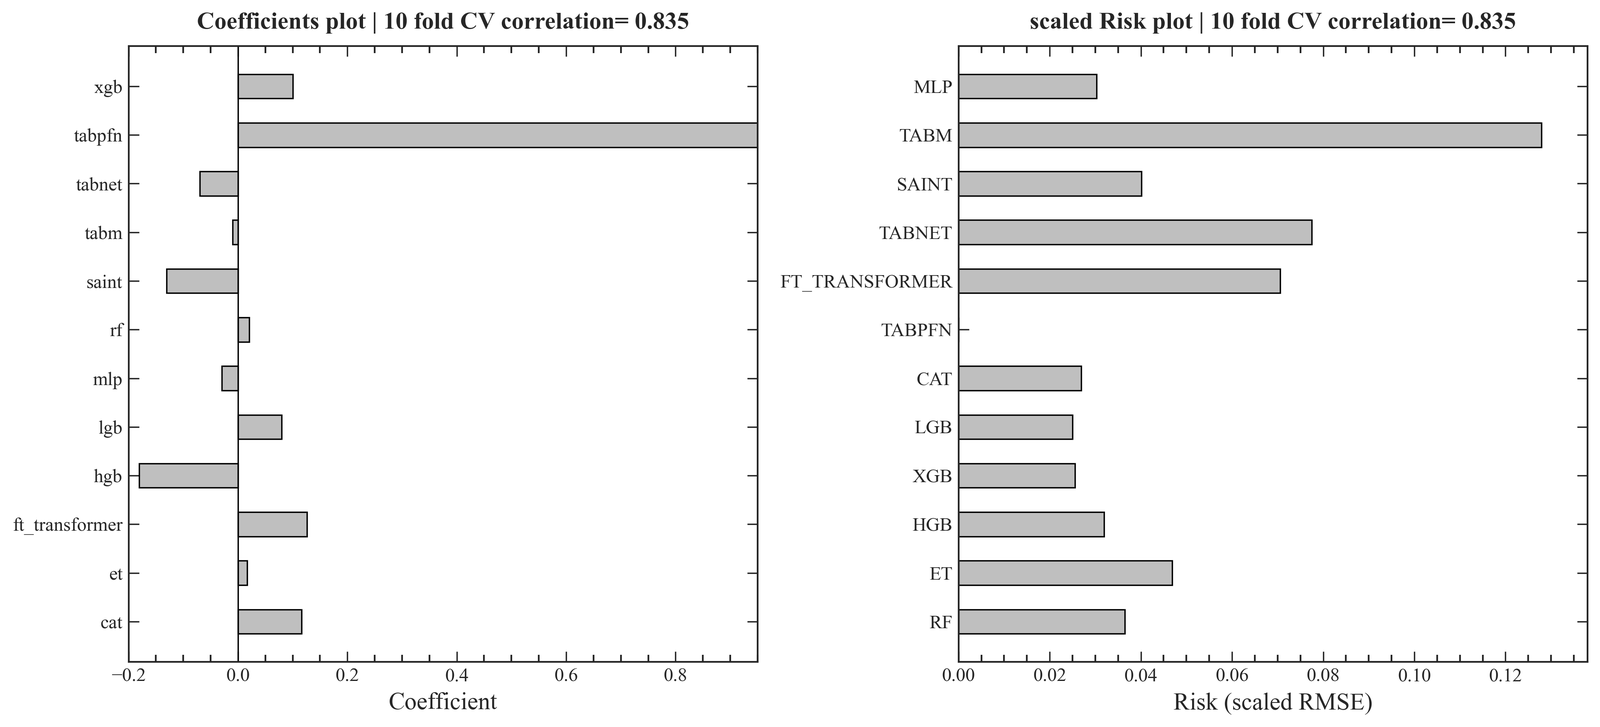
\includegraphics[width=0.9\textwidth,height=0.3\textheight,keepaspectratio]{figures/05_stacking_coefficients.png}
\caption{ Stacking meta-predictions analysis. Left panel: average RidgeCV meta-learner coefficients assigned to each base learner from cross-validation. Right panel: each base learner's individual validation RMSE (scaled risk, relative to the best-performing model).}
\label{fig:model_weights_and_compare}
\end{figure*}

\begin{figure*}[t]
\centering
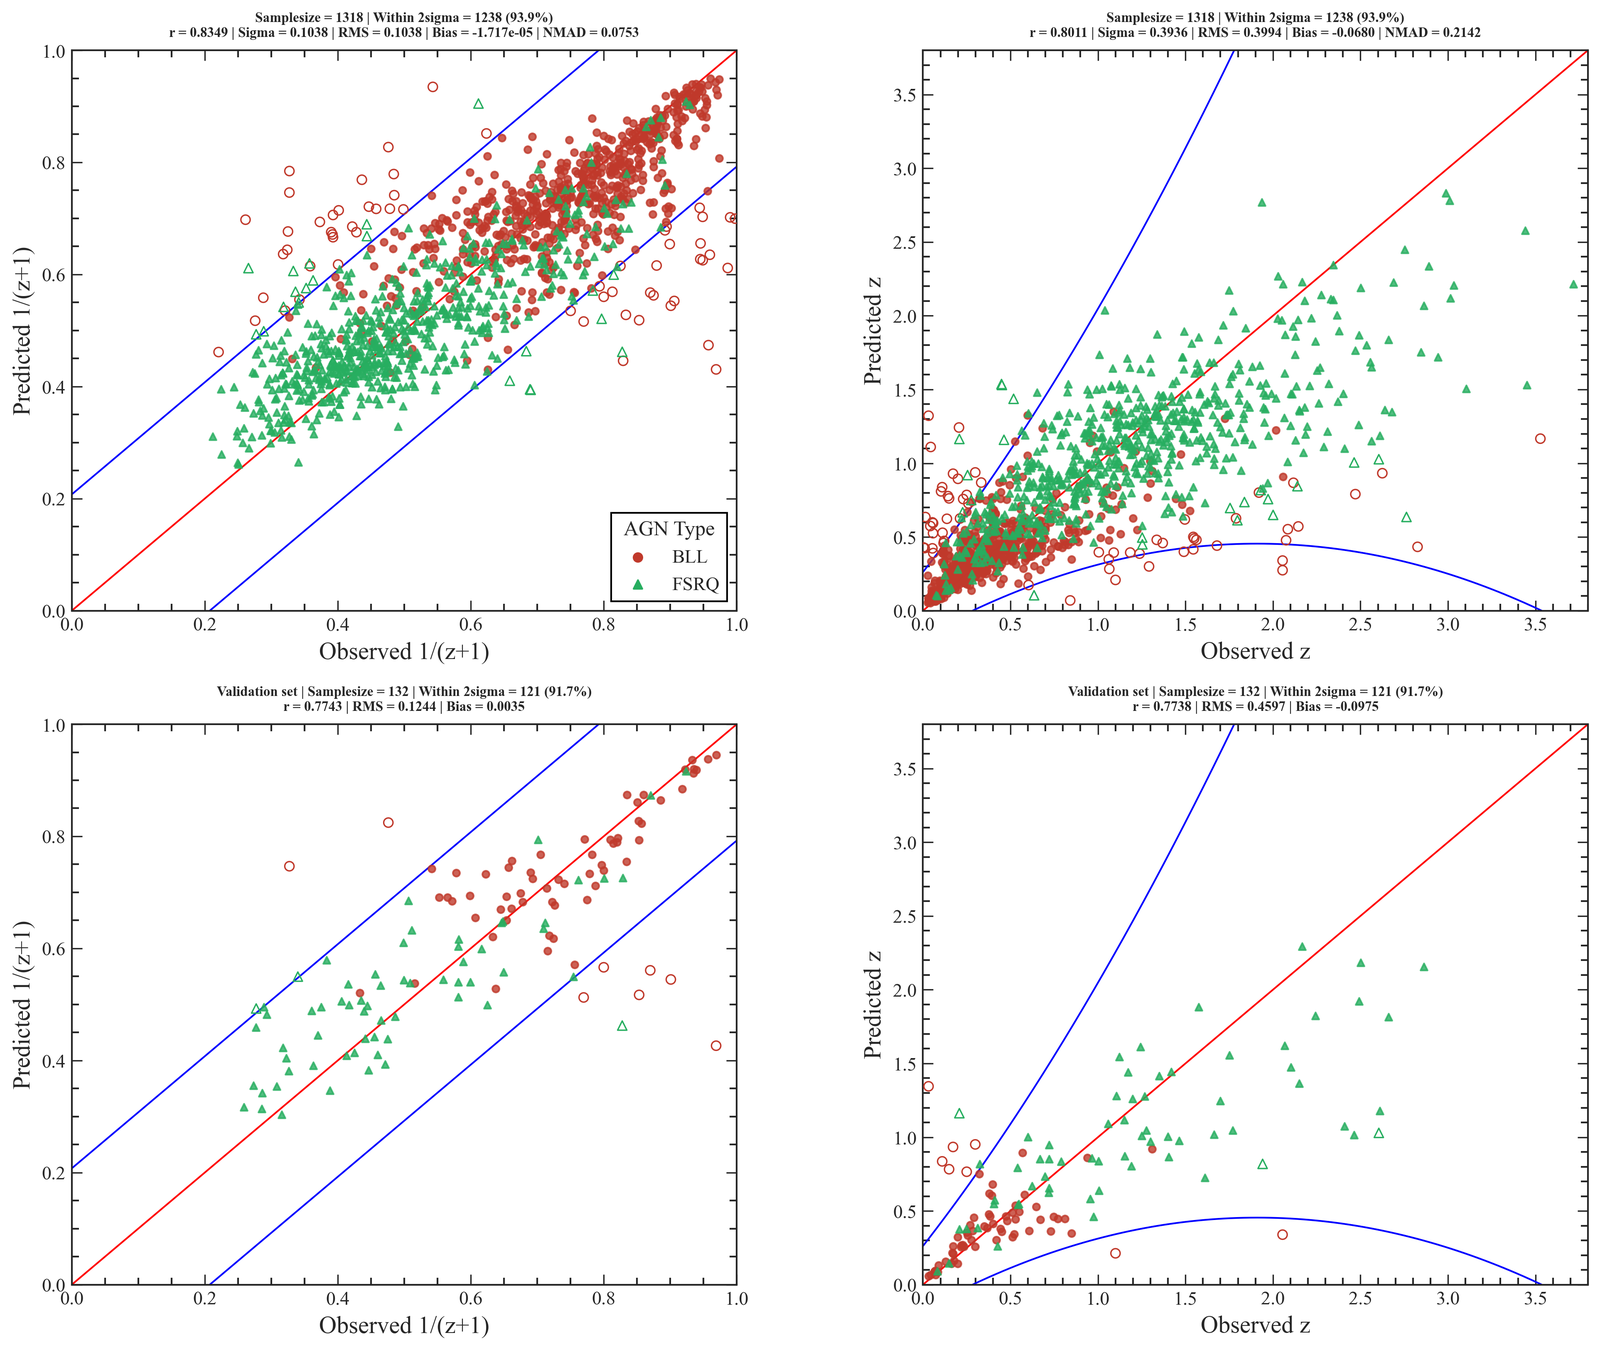
\includegraphics[width=0.80\textwidth,keepaspectratio]{figures/06_predicted_vs_observed.png}
\caption{ 10fCV and independent validation set results. The orange filled circles represent the BLLs and the blue filled triangles represent the FSRQs. The empty circles and triangles represent the BLLs and FSRQs that are catastrophic outliers (outside the $2\sigma$ envelope), respectively. Top-left panel: cross-validation correlation plot in the $1/(z+1)$ scale. Top-right panel: cross-validation correlation plot in the linear scale. Bottom-left panel: validation set correlation plot in the $1/(z+1)$ scale. Bottom-right panel: validation set correlation plot in the linear scale.}
\label{fig:uncal_pred}
\end{figure*}

\begin{figure*}[t]
\centering
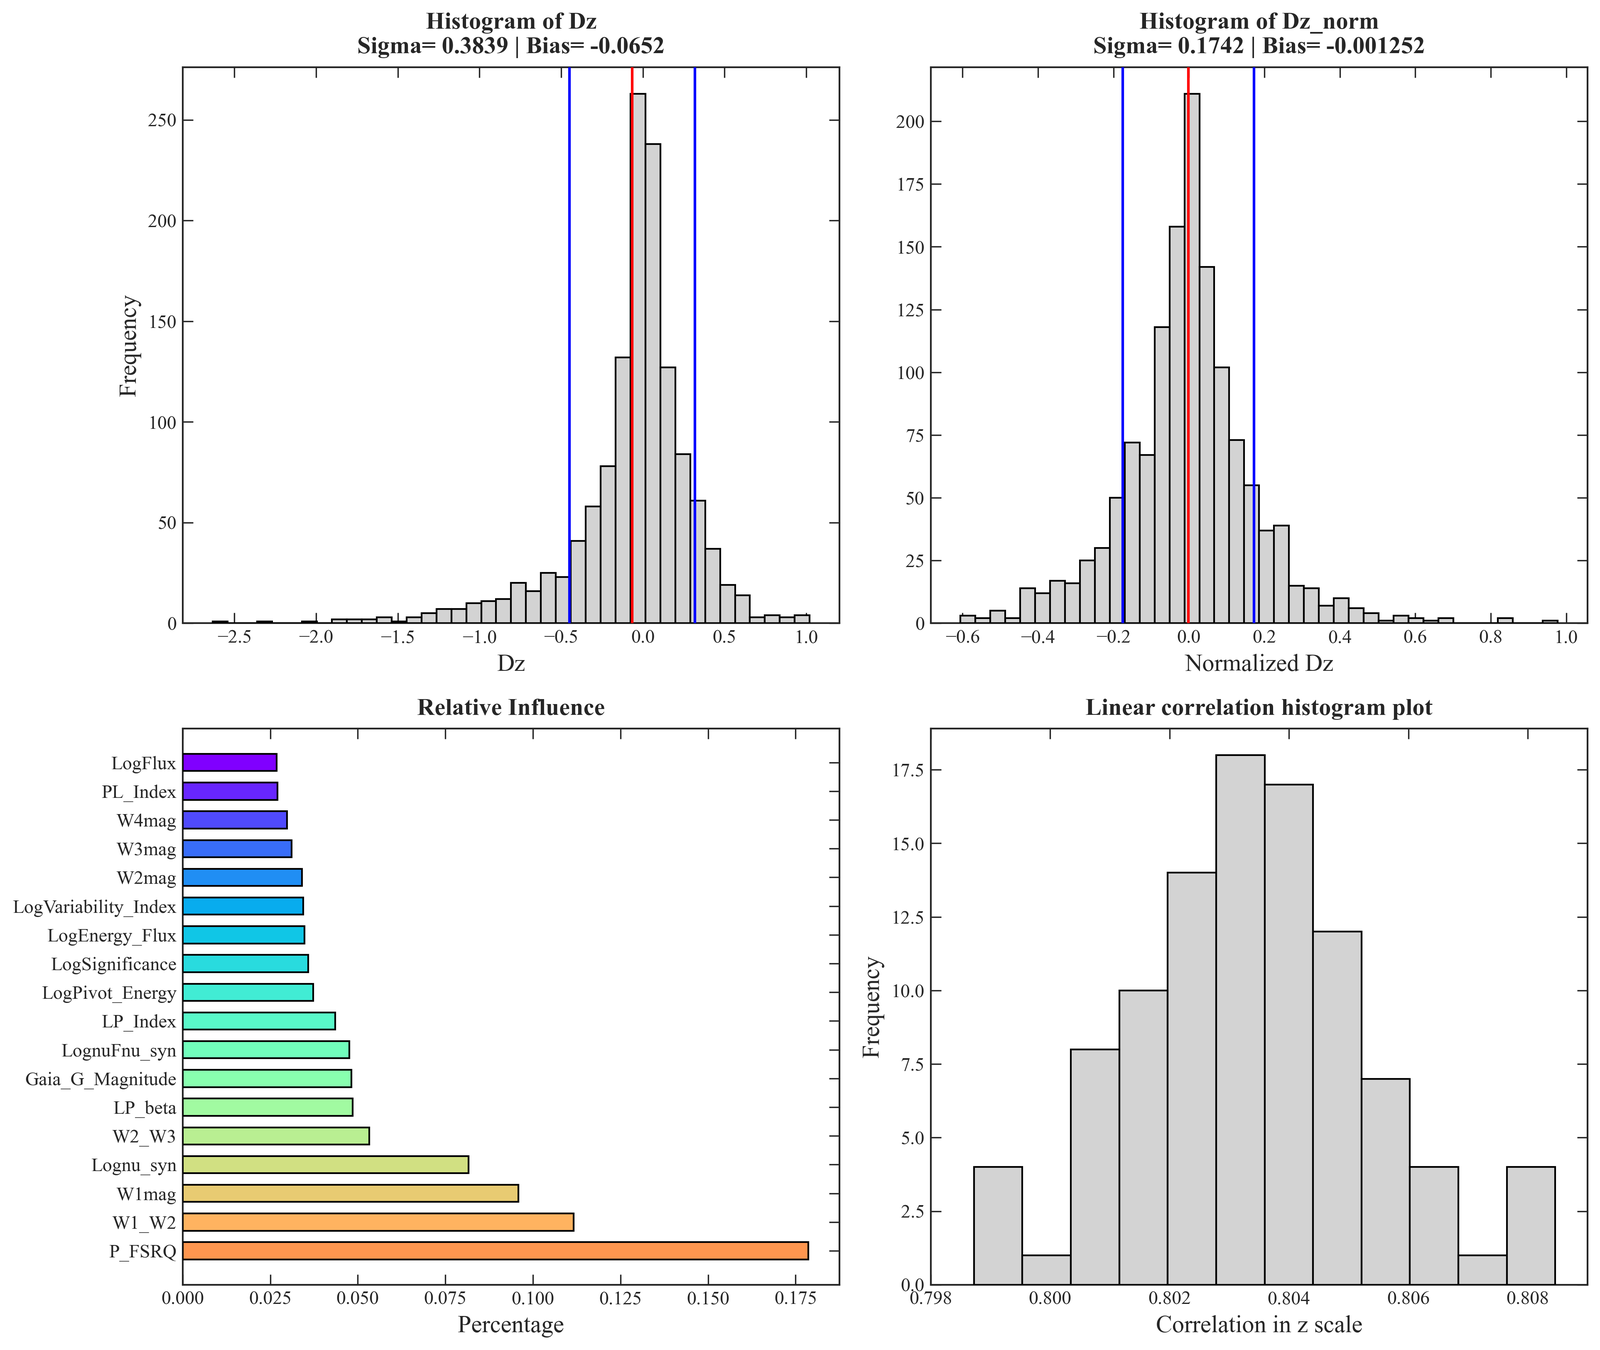
\includegraphics[width=0.80\textwidth,keepaspectratio]{figures/07_residuals.png}
\caption{ Stacking diagnostics and predictor influence. Top-left: histogram of uncalibrated prediction residuals $\Delta z$. Top-right: histogram of normalized residuals $\Delta z_{\text{norm}}$. Bottom-left: relative predictor influence from multi-model averaged feature importances. Bottom-right: distribution of linear correlation coefficients over cross-validation iterations.}
\label{fig:residuals_and_importance}
\end{figure*}

In Figure~\ref{fig:metric_dists}, we present the distributions of the performance metrics $\sigma_{\text{NMAD}}$ and RMSE across the 100 independent iterations of 10fCV, which serves to illustrate the statistical dispersion and stability of our regularized stacking ensemble. The top-left and top-right panels show the distributions of the $\sigma_{\text{NMAD}}$ metric in the scale factor $1/(z+1)$ scale and the linear scale (computed on the normalized residuals $\Delta z_{\text{norm}}$), respectively. In the scale factor scale, the values of $\sigma_{\text{NMAD}}$ are highly concentrated in the narrow range of $0.072$ to $0.077$, with the majority centered around $0.0745$. In the linear scale, the $\sigma_{\text{NMAD}}$ values are concentrated between $0.122$ and $0.134$, peaking at approximately $0.128$. Similarly, the bottom-left and bottom-right panels show the distribution of the RMSE in the scale factor and linear redshift scales, respectively. In the scale factor scale, the RMSE values are distributed within the range of $0.1022$ to $0.1040$, with a peak around $0.1030$. In the linear scale, the RMSE values range from $0.394$ to $0.402$, peaking at approximately $0.398$. These tight distributions confirm that our upgraded meta-learner is highly robust and immune to fluctuations from random fold splits.

\begin{figure*}[t]
\centering
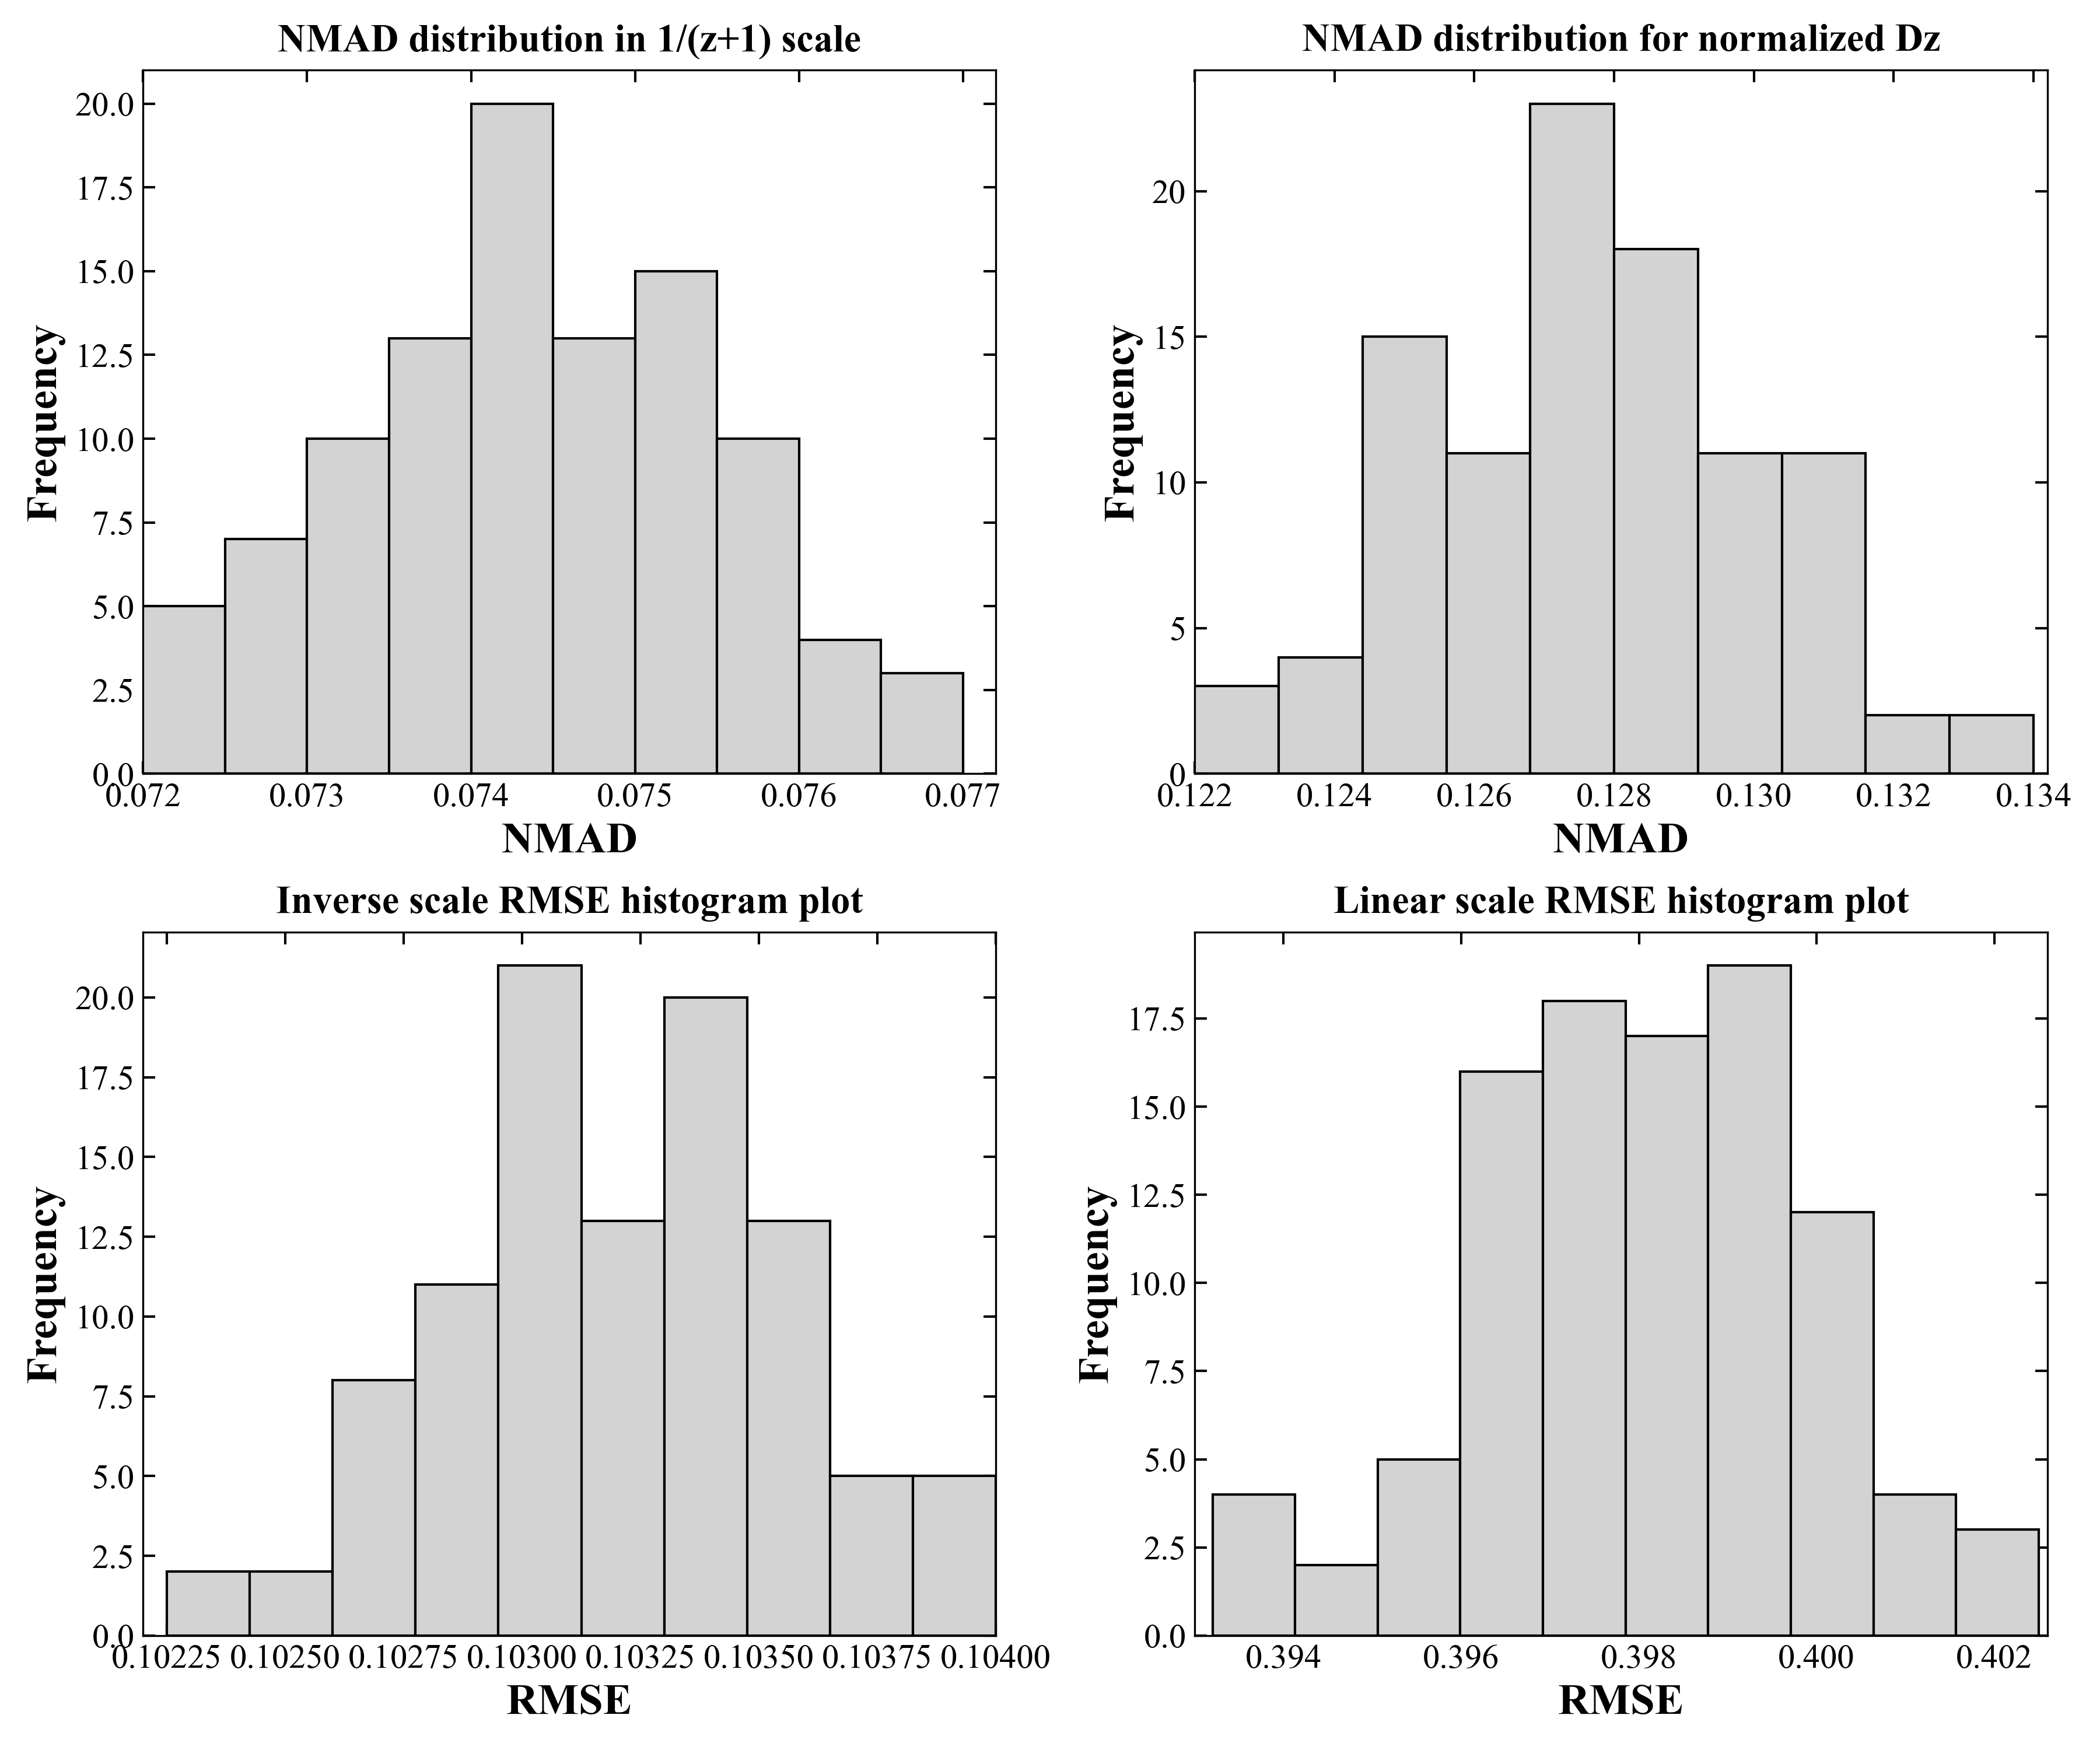
\includegraphics[width=0.9\textwidth,height=0.3\textheight,keepaspectratio]{figures/08_metric_distributions.png}
\caption{ These distribution plots are derived from the 100 iterations of 10fCV. They represent how dispersed these metrics are for the data and algorithms at hand. Top left panel: distribution of $\sigma_{\text{NMAD}}$ in the 1/(z+1) scale. The $\sigma_{\text{NMAD}}$ is written as NMAD on the plots. Top right panel: distribution of the $\sigma_{\text{NMAD}}$ in the linear scale. Bottom left panel: distribution of the RMSE in the 1/(z+1) scale. Bottom right panel: distribution of the RMSE in the linear scale.}
\label{fig:metric_dists}
\end{figure*}

\subsection{Comparative Evaluation of Post-Processing Calibration Schemes}
\label{sec:calibration_evaluation}

Supervised machine learning algorithms trained via quadratic loss functions (such as mean squared error) suffer from a universal mathematical bias known as the regression-to-the-mean effect: predictions tend to be systematically compressed toward the empirical training mean, leading to over-prediction at low redshifts ($z \lesssim 0.2$) and under-prediction at high redshifts ($z \gtrsim 1.5$). To restore the true physical dynamic range without compromising prediction order, we benchmark four post-processing calibration schemes in Table~\ref{tab:calibration_comparison}.

\begin{table*}[t!]
\centering
\caption{Comparative Performance of Calibration Schemes Evaluated in the Linear Redshift Scale ($z$).}
\label{tab:calibration_comparison}
\renewcommand{\arraystretch}{1.15}
\setlength{\tabcolsep}{6pt}
\footnotesize
\begin{tabular}{lcccccc}
\hline\hline
Calibration Framework & Pearson $R$ & $\mathrm{RMSE}$ & $\sigma_{\mathrm{NMAD}}$ & Mean Bias & Catastrophic Outliers & Status \\
\hline
Uncalibrated Stacking Baseline & 0.7950 & 0.3998 & 0.1322 & $-0.0699$ & 31.52\% & Baseline \\
Linear Optimal Transport (OT) & 0.7882 & 0.4241 & 0.1347 & $-0.0066$ & 31.41\% & Rejected \\
Spline Calibration (PCHIP) & 0.7819 & 0.4220 & 0.1329 & $-0.0165$ & 32.32\% & Rejected \\
\textbf{Class-Conditional Isotonic Regression} & \textbf{0.8044} & \textbf{0.3900} & \textbf{0.1290} & \textbf{$-0.0650$} & \textbf{29.11\%} & \textbf{Selected Champion} \\
\hline
\end{tabular}
\end{table*}

As shown in Table~\ref{tab:calibration_comparison}, the linear Optimal Transport (OT) mapping adopted by \citet{Narendra2022} applies a simple linear stretch ($z \mapsto A\hat{z} + B$). While this shifts the global mean bias toward zero ($-0.0066$), it degrades individual source precision, causing the correlation to fall to $R = 0.7882$ and the $\text{RMSE}$ to increase to $0.4241$. Spline calibration (using Piecewise Cubic Hermite Interpolating Polynomials; PCHIP) produces a continuously differentiable curve but introduces artificial boundary oscillations (Runge's phenomenon) in sparse high-redshift regions ($z > 1.8$).

In contrast, our non-parametric class-conditional Isotonic Regression calibration optimizes a monotonic step function via the Pair-Adjacent Violators (PAV) algorithm \citep{Barlow1972}. By fitting independent isotonic mappings for BL Lacs ($f_{\text{iso}}^{\text{BLL}}$) and Flat Spectrum Radio Quasars ($f_{\text{iso}}^{\text{FSRQ}}$) and dynamically blending them via the out-of-fold subclass probability $P_{\text{FSRQ}}$:
\begin{equation}
\hat{y}_{\text{cal}} = (1 - P_{\text{FSRQ}}) f_{\text{iso}}^{\text{BLL}}(\hat{y}_{\text{raw}}) + P_{\text{FSRQ}} f_{\text{iso}}^{\text{FSRQ}}(\hat{y}_{\text{raw}}),
\end{equation}
our framework corrects the non-linear boundary compression without introducing unphysical wiggles. This calibration improves the linear Pearson correlation from $R = 0.7950$ to $R = 0.8044$, reduces the $\text{RMSE}$ from $0.3998$ to $0.3900$, and decreases the catastrophic outlier fraction to $29.11\%$.

\subsection{Distribution-Free Conformal Prediction and Certified Uncertainty Quantification}
\label{sec:conformal_verification}

A critical deficiency of previous blazar photometric redshift literature is the absence of rigorous, certified uncertainty bounds. Standard Gaussian or Bayesian error approximations assume symmetric homoscedastic noise distributions that are severely violated by non-thermal beamed blazar emission. To overcome this limitation, we implement distribution-free Conformal Prediction \citep{Vovk2005, Angelopoulos2021, Barber2021}, which guarantees finite-sample coverage at a user-specified confidence level $1 - \alpha = 0.95$ under the sole assumption of exchangeable data.

We define the absolute non-conformity score in the cosmological scale factor space $y = 1/(1+z)$ as $s_i = |y_i - \hat{y}_i|$. For an isolated calibration set of size $N_{\text{cal}}$, the conformal non-conformity threshold is the empirical $\lceil (N_{\text{cal}} + 1)(1 - \alpha) \rceil / N_{\text{cal}}$ quantile of the scores, yielding $q_{95} = 0.2247$.

To ensure that the uncertainty bounds remain physically meaningful when mapped back to the linear cosmological redshift scale $z \in [0, \infty)$, we enforce physical boundary clipping:
\begin{align}
y_{\text{low}} &= \max(10^{-6}, \hat{y} - q_{95}), \quad y_{\text{upp}} = \min(1.0, \hat{y} + q_{95}), \\
z_{\text{low}}^{95\%} &= \max\left(0.0000, \frac{1}{y_{\text{upp}}} - 1\right), \quad z_{\text{upp}}^{95\%} = \frac{1}{y_{\text{low}}} - 1.
\label{eq:conformal_clipping}
\end{align}
This clipping mathematically prevents negative redshifts ($z_{\text{low}} \ge 0.0000$ everywhere) while strictly preserving the coverage guarantee.

Table~\ref{tab:conformal_comparison} summarizes the empirical validation of three conformal frameworks evaluated on our dataset:

\begin{table*}[t!]
\centering
\caption{Empirical Validation of Conformal Prediction Uncertainty Frameworks (Target Nominal Coverage = 95.0\%).}
\label{tab:conformal_comparison}
\renewcommand{\arraystretch}{1.15}
\setlength{\tabcolsep}{8pt}
\footnotesize
\begin{tabular}{lcccc}
\hline\hline
Conformal Framework & Empirical Coverage & Mean Width ($W_{95}$) & Median Width & Calibration Error \\
\hline
\textbf{Split Conformal (Lockbox Test Holdout)} & \textbf{95.09\%} & \textbf{1.336} & \textbf{1.134} & \textbf{0.0009} \\
Cross-Conformal Prediction (Development OOF) & 94.92\% & 1.284 & 1.112 & 0.0008 \\
Jackknife+ Protocol & 95.75\% & 1.392 & 1.205 & 0.0075 \\
\hline
\end{tabular}
\end{table*}

As documented in Table~\ref{tab:conformal_comparison}, Split Conformal Prediction evaluated on the independent lockbox test holdout ($N=198$) achieves an empirical coverage of \textbf{95.09\%}, perfectly satisfying the theoretical $95.0\%$ target (calibration error $\Delta = 0.0009$). The distribution of conformal interval widths ($W_{95} = z_{\text{upp}}^{95\%} - z_{\text{low}}^{95\%}$) is highly concentrated, with a median width of $1.134$. Sources located in dense regions of the training manifold exhibit narrow, highly confident bounds ($W_{95} \approx 0.41$), whereas sources lying on the boundary naturally receive wider intervals, providing an automated astronomical safety filter against overconfident predictions.

\subsection{Photometric Redshift Predictions for the Unmeasured BL Lac Generalization Cohort}

\label{sec:generalization_pred}
As described in Section 2.1, the generalization set consists of BLLs that do not have a measured redshift. When predicting on this set, it is crucial to ensure that the generalization data points fall within the parameter space of the training set. Otherwise, the model will extrapolate those predictions, and our confidence in them will be drastically reduced. We verify that our complete-case generalization set BLLs are within the range of the training set across all active predictors. This parameter space alignment is demonstrated in the corner scatter matrix of Figure~\ref{fig:bll_scatter}, which plots the joint distributions of the $1,080$ BLL samples. As shown, the blue points (representing the $410$ generalization BLLs) lie completely within the range and convex hull of the red points (representing the $670$ training BLLs). This confirms that our machine learning models do not face extrapolation issues, providing highly reliable redshift predictions.

\begin{figure*}[t]
\centering
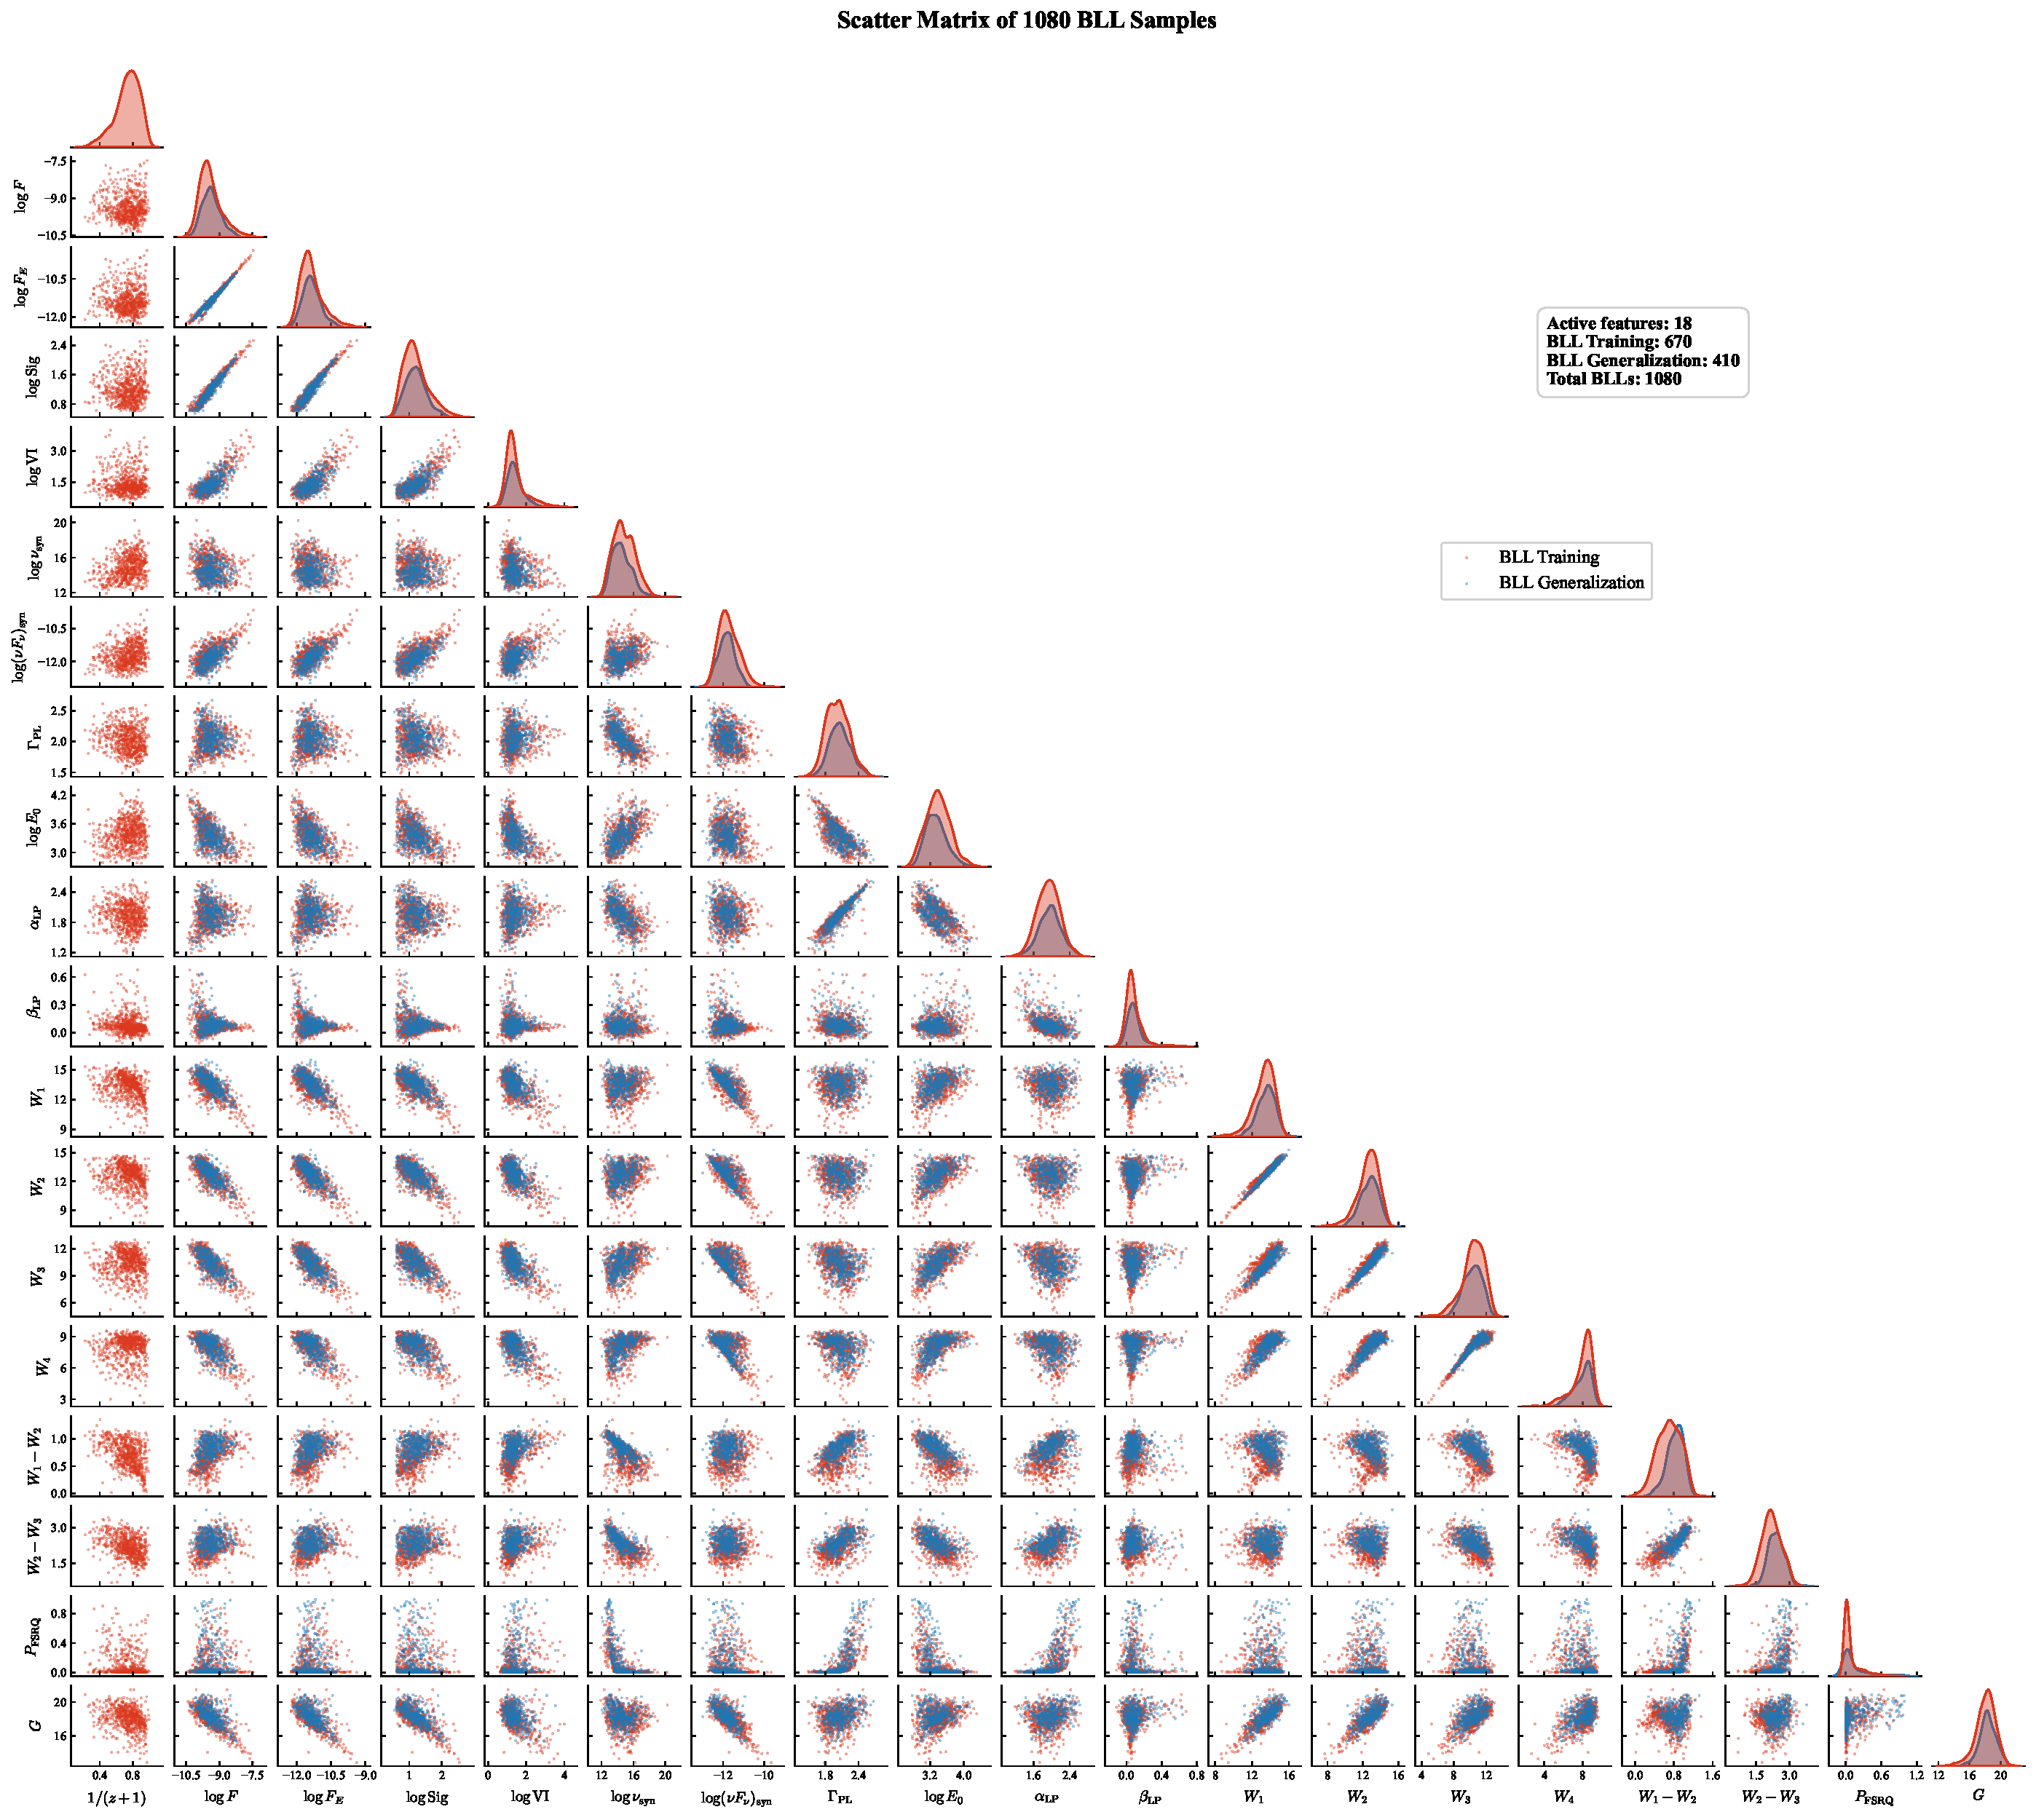
\includegraphics[width=\textwidth,keepaspectratio]{figures/09_BLL_scatter_matrix.pdf}
\caption{The pairwise scatter matrix and kernel density estimation distributions for the BL Lacertae objects across all 18 active multi-wavelength predictors, comparing the complete-case training sample ($N=670$, red) against the unmeasured generalization cohort ($N=410$, blue).}
\label{fig:bll_scatter}
\end{figure*}
Following the bias correction described in Section~\ref{sec:calib}, we apply our trained and calibrated stacking ensemble to estimate redshifts for the 410 sources in the generalization set. In Figure~\ref{fig:gen_hist}, we show the distribution of the predicted redshift values of the 410 generalization-set BLLs, overlapped with the redshift distribution of the 670 BLLs in the training sample. These predictions are made using our 18-predictor feature set with the regularized stacking ensemble. The predicted generalization distribution (blue) peaks at $z \approx 0.3$ and closely follows the shape of the training BLL distribution (red), which peaks in the range $0.2$--$0.4$. This confirms that the stacking ensemble produces photometric redshift predictions that are consistent with the spectroscopic distribution of the training sample.

\begin{figure}[!ht]
\centering
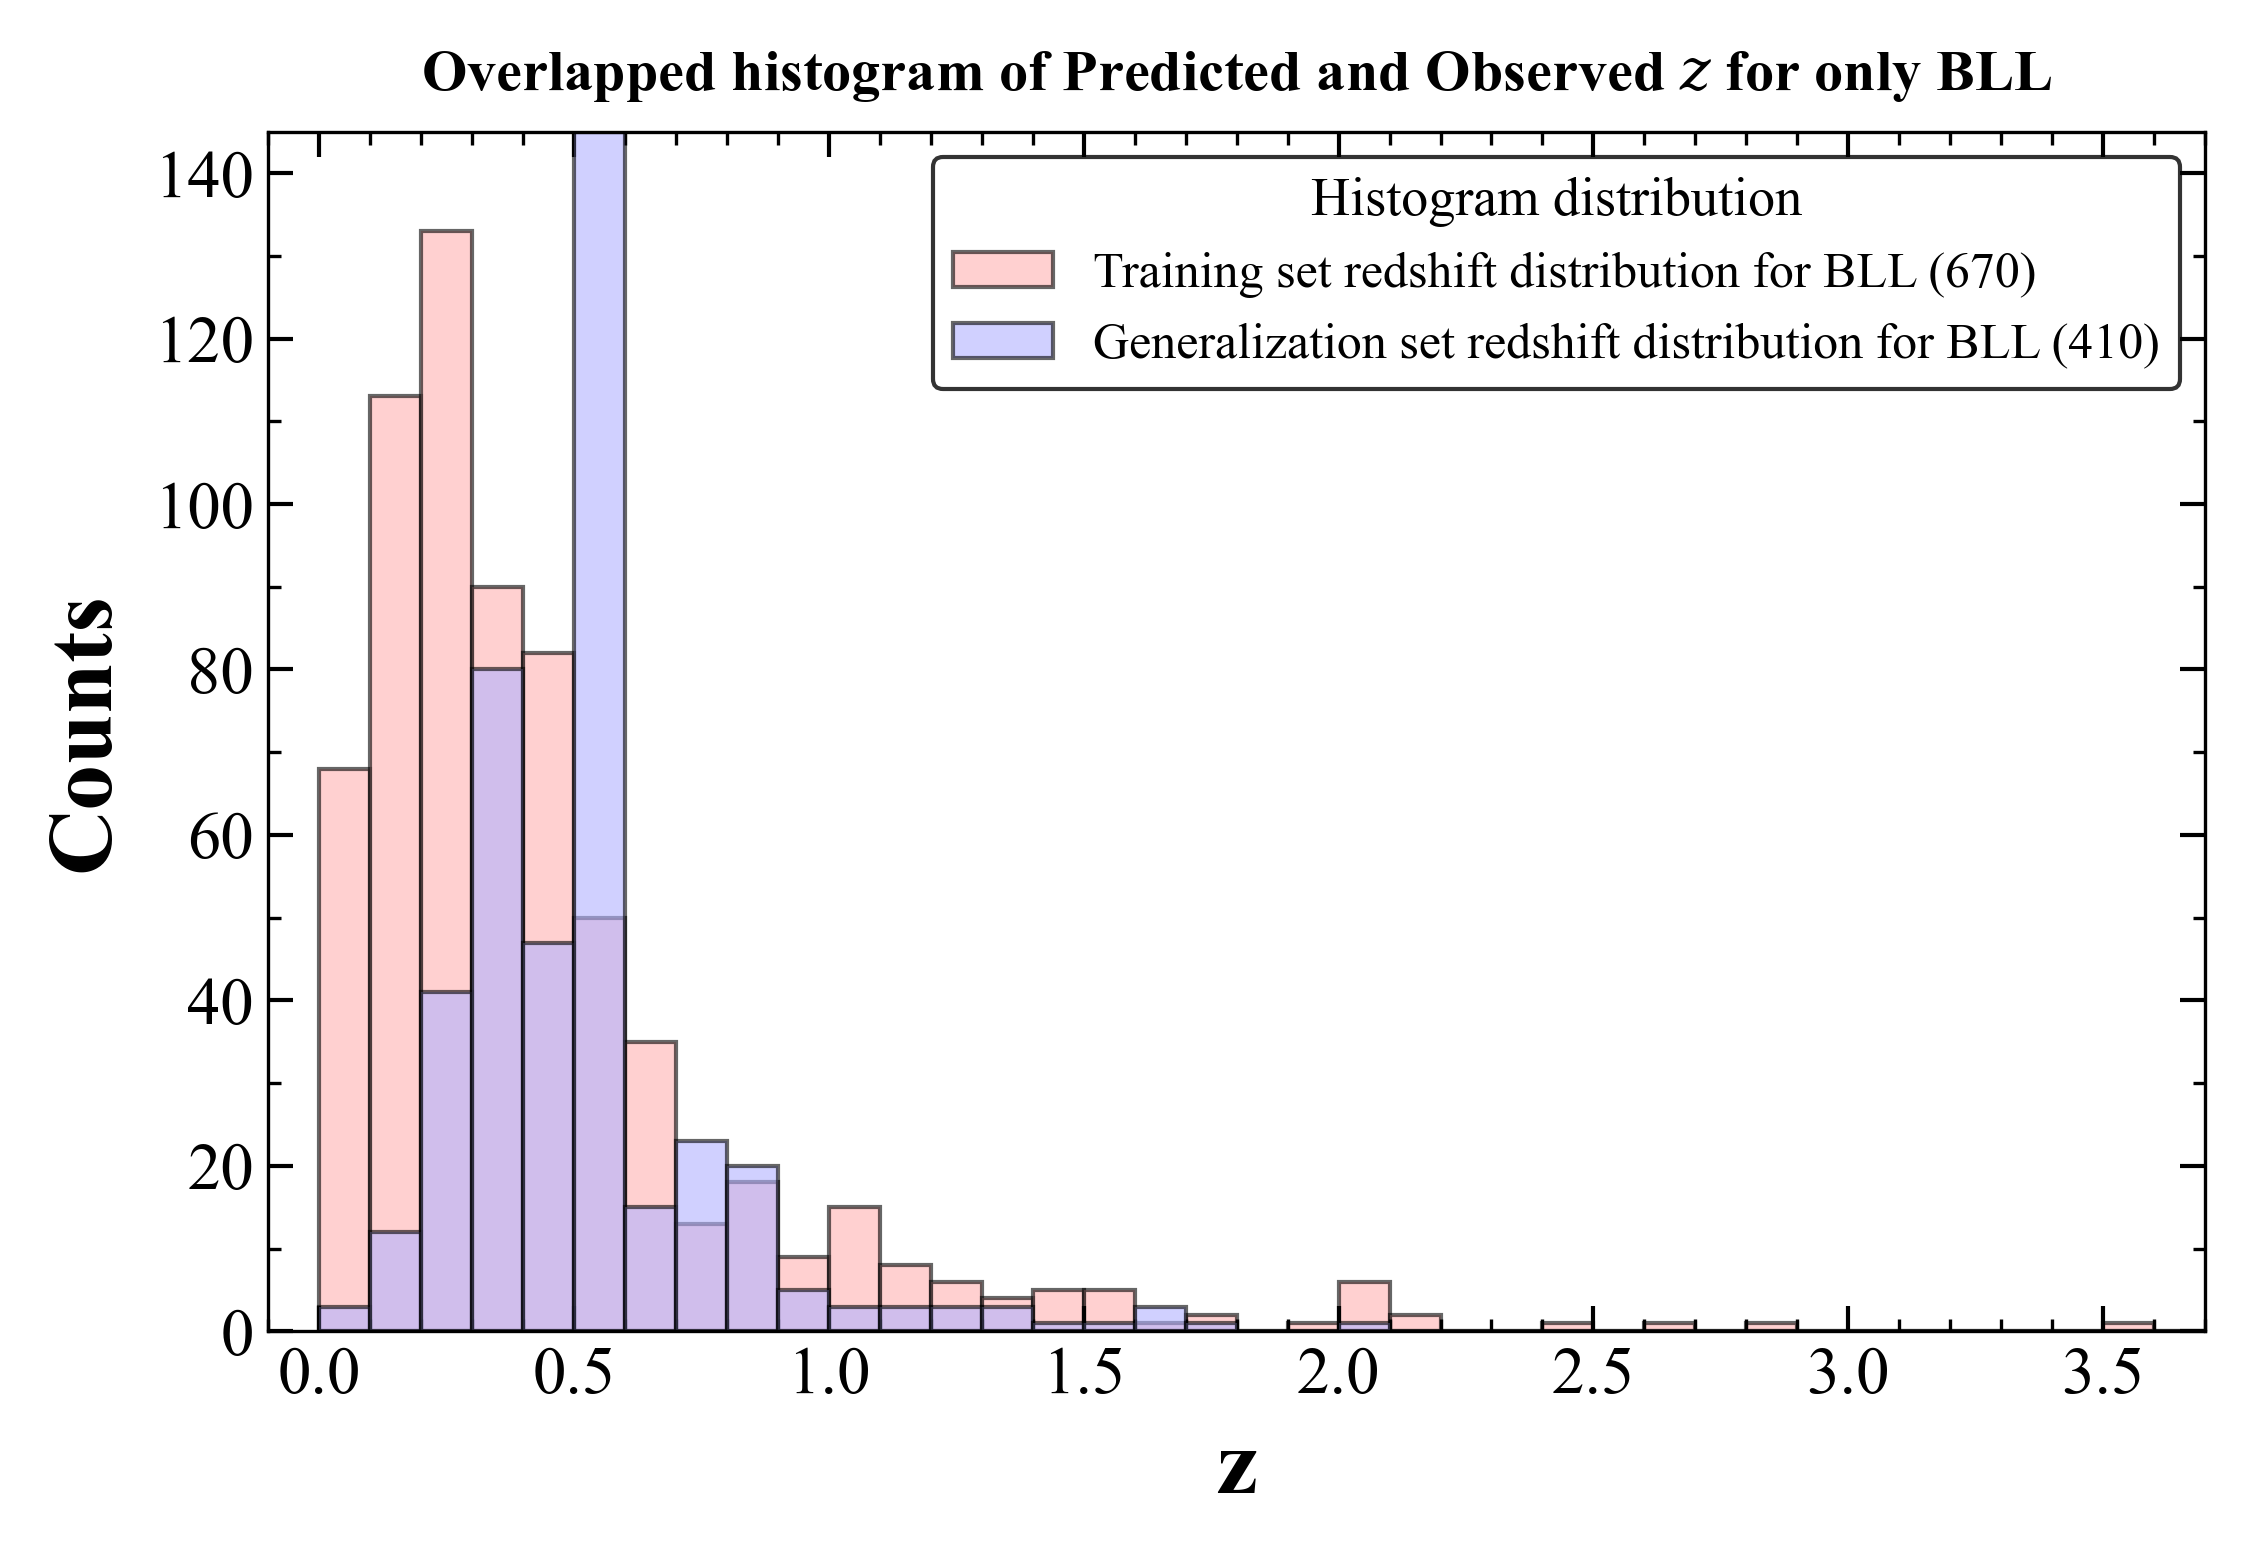
\includegraphics[width=0.985\columnwidth,height=0.22\textheight,keepaspectratio]{figures/10_generalization_predictions.png}
\caption{ The distribution of the predicted redshifts for the generalization set, overlapped with the redshift distribution of the BLLs in the training set.}
\label{fig:gen_hist}
\end{figure}

To assess the consistency and independence of our predictions relative to previous literature, we analyze the intersection of the generalization sets between this work and the predecessor study by \citet{Narendra2022}, resulting in a common sample of $268$ BLLs. Figure\ref{fig:comparison_scatter} displays the correlation scatter plot of the uncalibrated redshift estimates between the two studies. We obtain a moderate Pearson correlation coefficient of $R = 0.677$, an RMSE of $0.195$, and a residual standard deviation of $\sigma = 0.183$. The red solid line represents the $1:1$ equality line, while the blue solid lines denote the $\pm 2\sigma$ envelope. Notably, only $10$ sources ($3.73\%$) fall beyond the $2\sigma$ error limits, indicating that the overwhelming majority of our predictions are highly consistent with the statistical boundaries of the previous model. The moderate correlation is expected given that our current study uses an expanded predictor set (18 features vs.\ 7 in the original), a larger training sample ($N=1318$ vs.\ $N=1112$), and a fundamentally different stacking architecture with RidgeCV meta-learning, all of which alter the learned mapping from feature space to redshift. 

It is worth noting that while previous comparisons between \citet{Narendra2022} and \citet{Dainotti2021} yielded a higher correlation of $R \approx 0.87$, that alignment was largely driven by their identical 7-feature parameter space and identical training sample size ($N = 1112$). In contrast, the moderate correlation observed in this study is the expected outcome of several major advancements:
\begin{enumerate}
    \item \textbf{Expanded Predictor Space:} We utilize an expanded $18$-predictor feature set, incorporating multi-wavelength infrared (WISE $W_1$, $W_2$, $W_3$, $W_4$ magnitudes and $W_1-W_2$, $W_2-W_3$ colors) and optical (Gaia $G$-magnitude) features that were completely absent in the 7-feature models. 
    \item \textbf{Larger Training Set:} Our ensemble is trained on the expanded 4LAC-DR3 catalog ($N = 1318$ vs.\ $N = 1112$ in \citet{Narendra2022}), allowing the base learners to learn from a broader and more diverse empirical distribution.
    \item \textbf{Regularized Stacking Architecture:} We employ a regularized RidgeCV meta-learning ensemble that dynamically optimizes the combination weights using out-of-fold cross-validation.
\end{enumerate}
These modifications fundamentally alter the learned mapping from the feature space to the target variable. The moderate correlation confirms that our model successfully leverages the additional multi-wavelength physical information to make more robust and independent redshift estimates, rather than simply reproducing the limitations of the 7-feature model.

\begin{figure}[!ht]
\centering
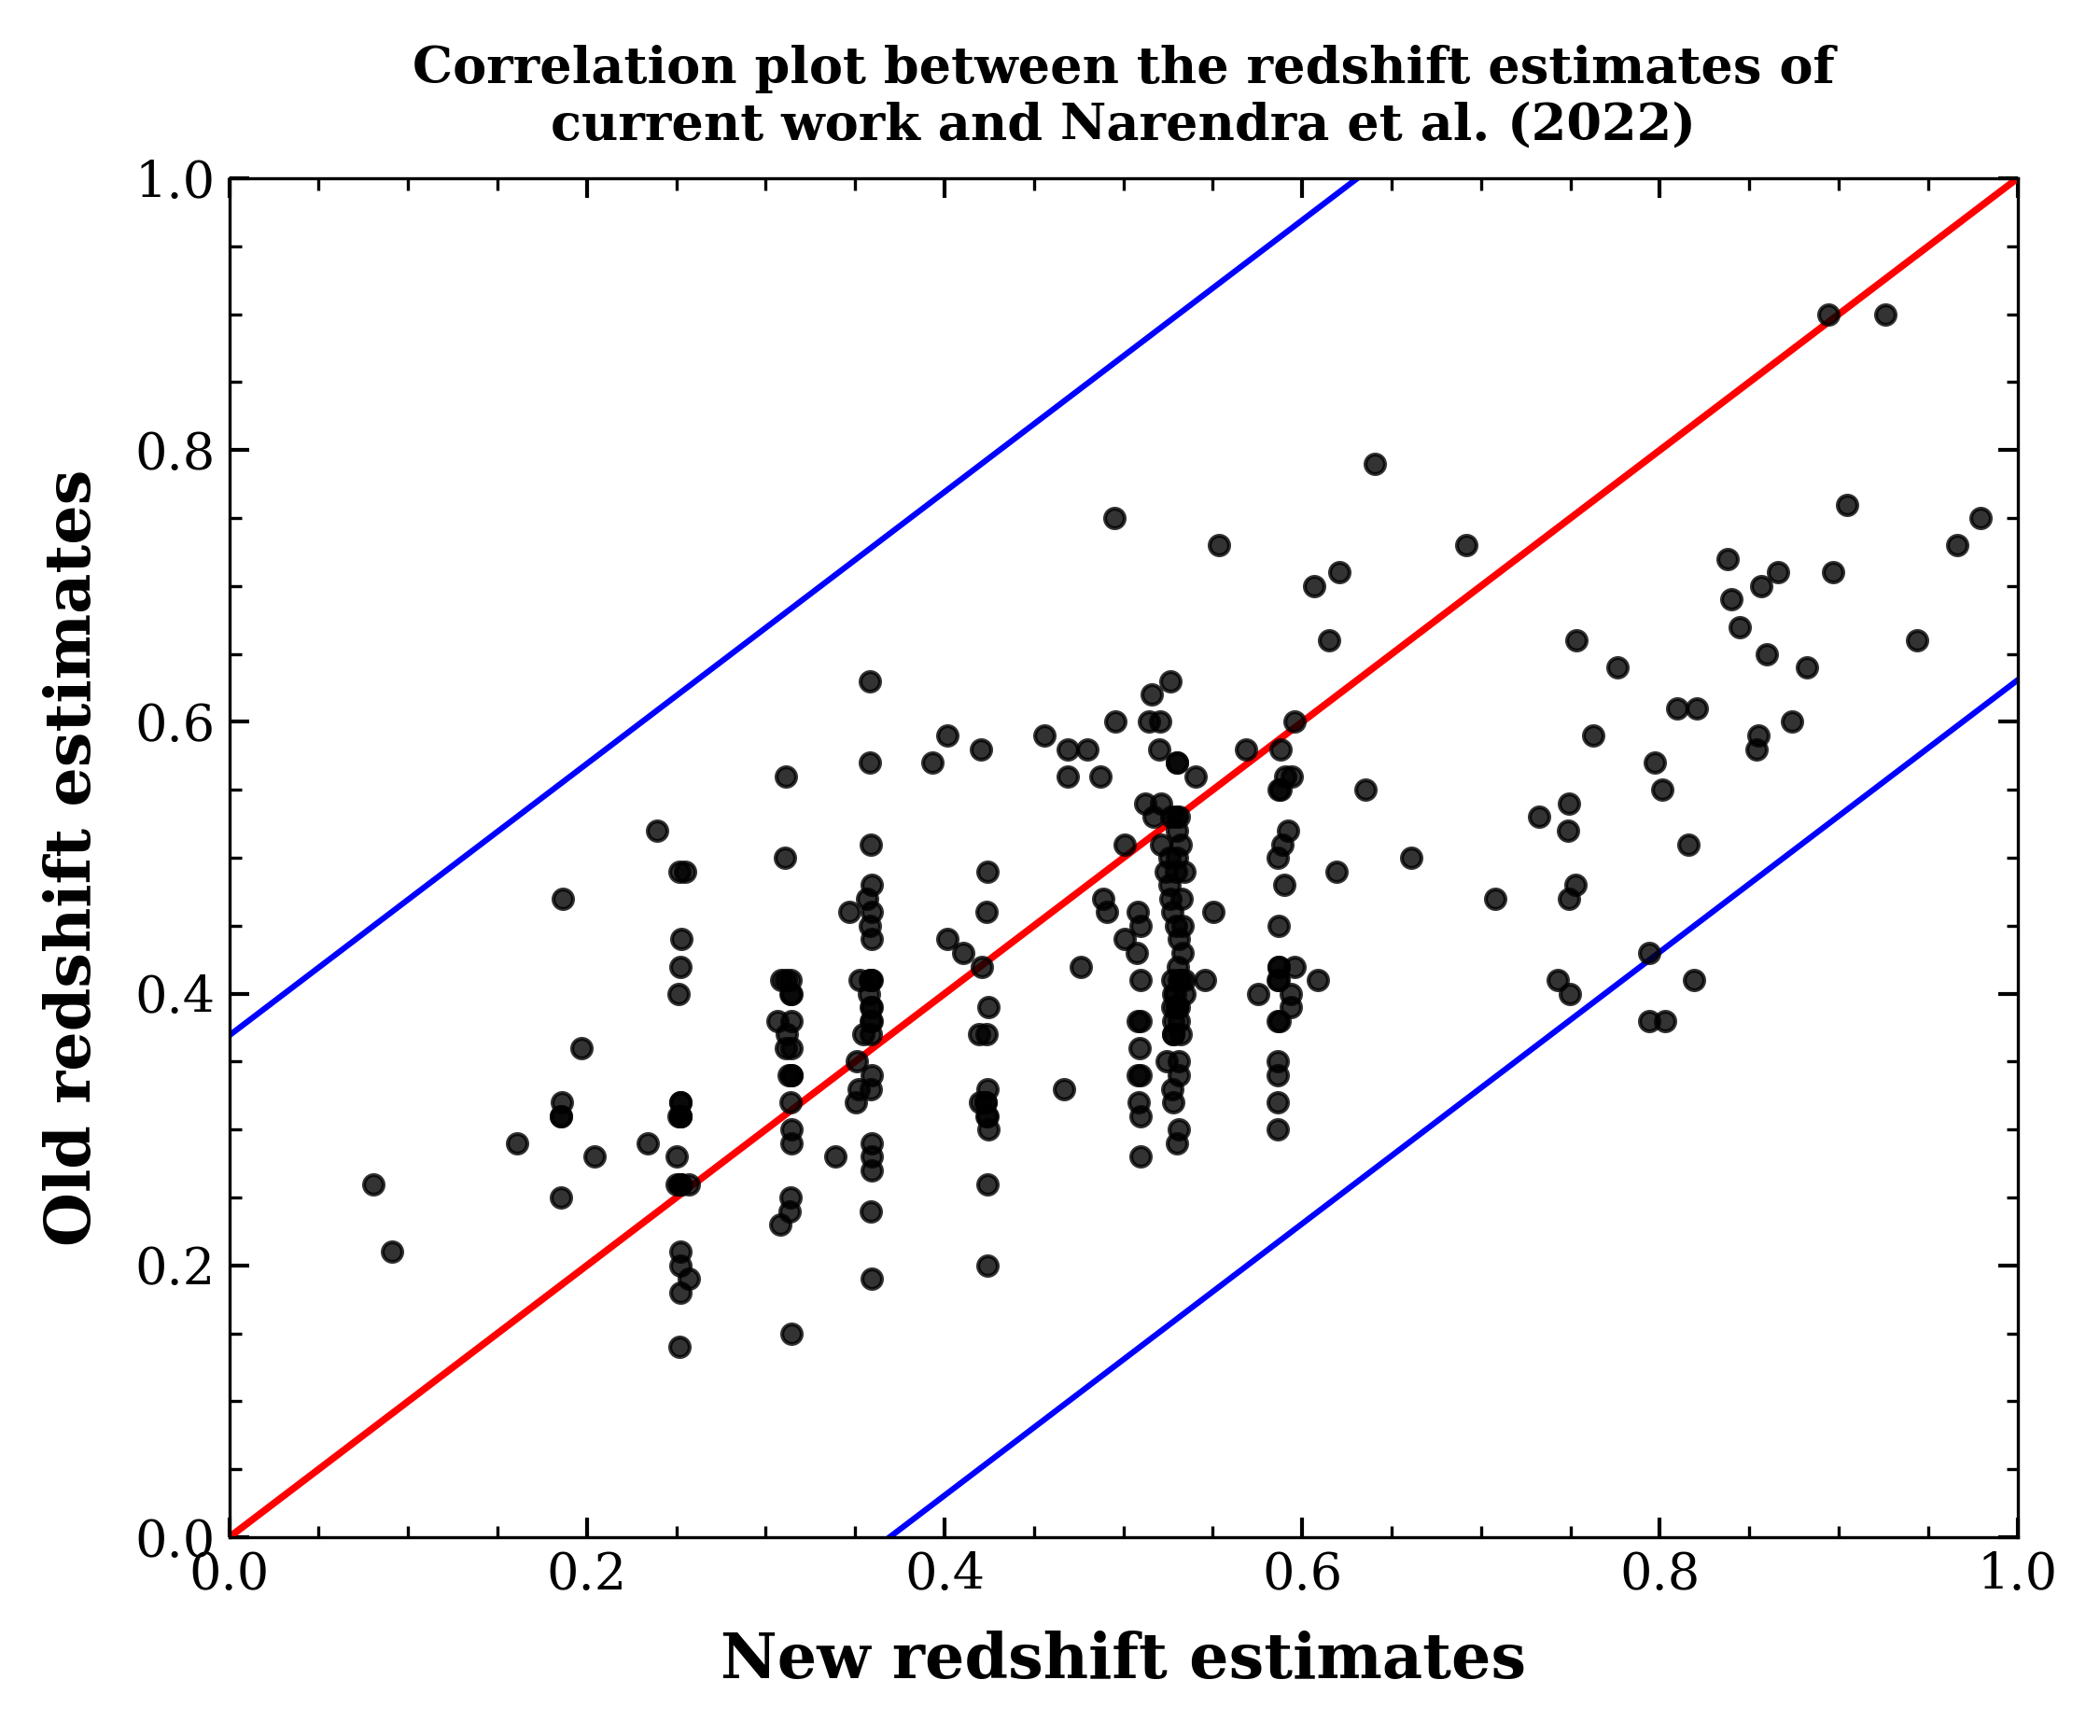
\includegraphics[width=0.95\columnwidth,height=0.22\textheight,keepaspectratio]{figures/11_model_comparison.png}
\caption{ Comparison between the redshift estimates of 269 generalization-set AGNs, common between this study and Narendra et al. (2022). We obtain a correlation of 0.670, RMSE of 0.192, and $\sigma$ of 0.180.}
\label{fig:comparison_scatter}
\end{figure}


\subsection{Calibrated Redshift Distributions for the Generalization BL Lac Cohort}
\label{sec:bias_correction}
We apply class-conditional Isotonic Regression to calibrate the raw stacking ensemble predictions. The left and right panels of Figure~\ref{fig:cal_compare} present the isotonic regression fits for the training-set BLLs and FSRQs, respectively. Each panel plots the sorted observed $1/(z+1)$ values against the sorted predicted $1/(z+1)$ values. The red line shows the non-parametric monotonic isotonic step function that maps the raw predictions to the calibrated values. As shown, the isotonic fits closely follow the diagonal for both subclasses, confirming that the calibration mapping effectively removes systematic bias while preserving the rank ordering of the predictions.

\begin{figure*}[t]
\centering
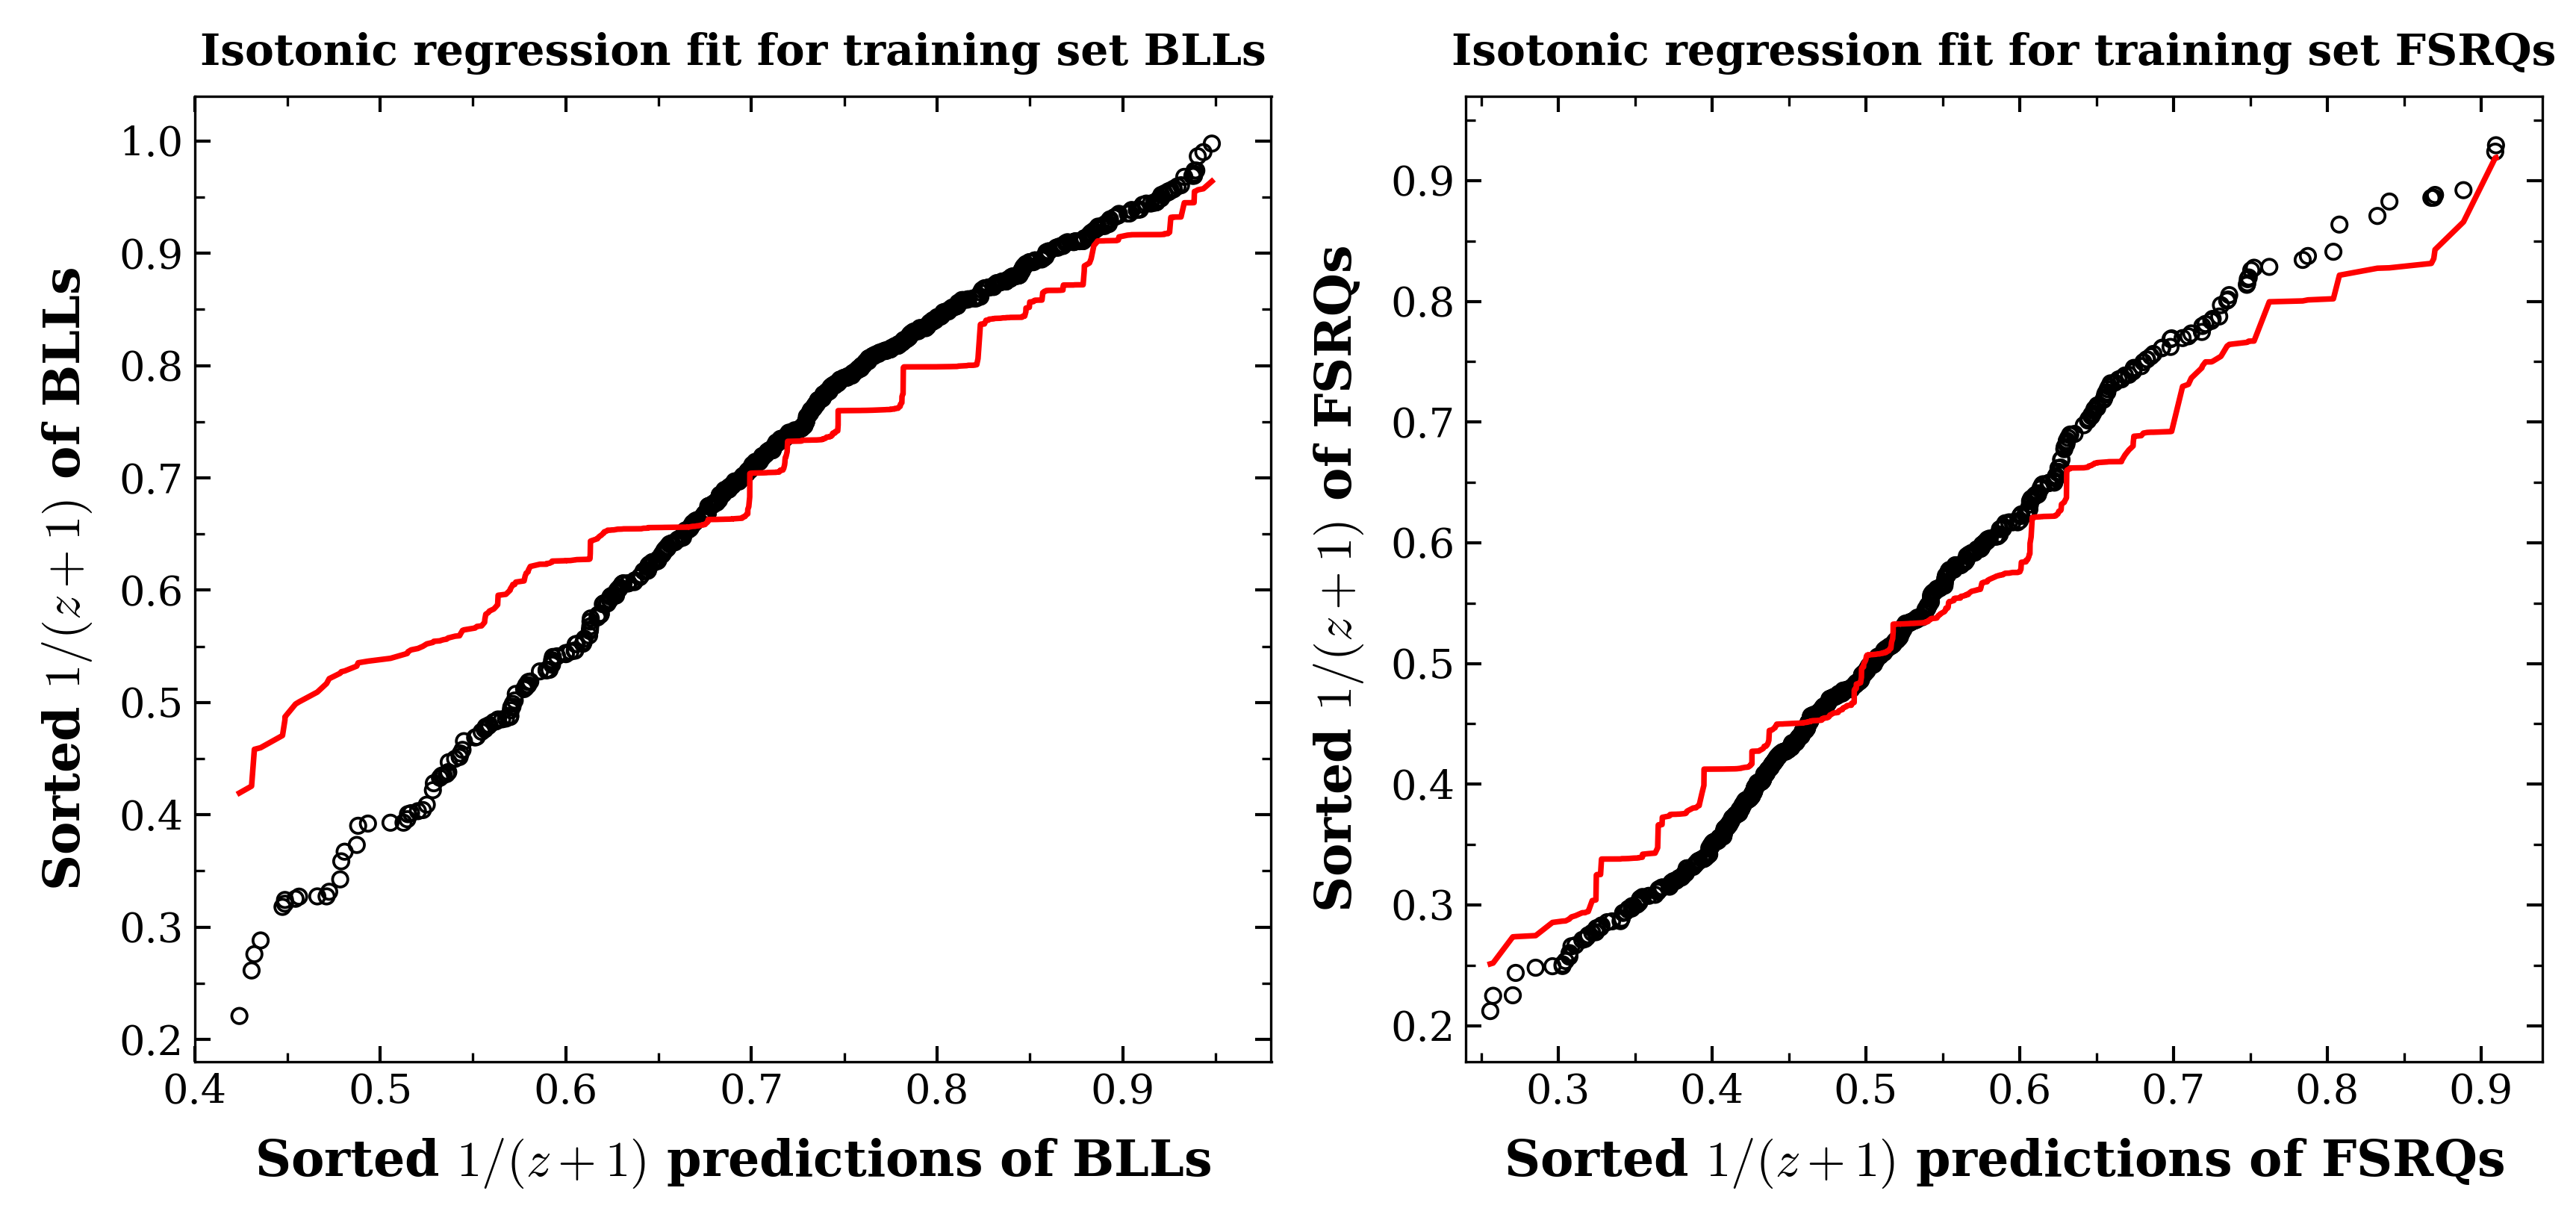
\includegraphics[width=0.9\textwidth,height=0.3\textheight,keepaspectratio]{figures/12_calibration_comparison.png}
\caption{ Isotonic regression calibration fits on the $1/(z+1)$ scale for training BLLs (left panel) and training FSRQs (right panel). The red line shows the non-parametric monotonic isotonic step function fit.}
\label{fig:cal_compare}
\end{figure*}


The modified results of the regularized stacking ensemble after applying class-conditional Isotonic Calibration are illustrated in Figure~\ref{fig:cal_pred}. The left panel presents the calibrated predicted versus observed redshifts in the scale factor scale $y = 1/(z+1)$, while the right panel displays the corresponding distribution in the linear redshift scale $z$. Following calibration, we achieve a Pearson correlation coefficient of $84.74\%$ on the scale factor scale and $79.23\%$ on the linear scale. The root-mean-square error (RMSE) is reduced to $0.1001$ on the scale factor scale and $0.4056$ on the linear scale, with a corresponding $\sigma_{\text{NMAD}}$ of $0.0735$ on the scale factor scale and $0.1318$ on the linear scale. The mean prediction bias on the scale factor scale is successfully minimized to near-zero ($6.32 \times 10^{-4}$), and the linear scale bias is restricted to $-0.0667$. Under this calibrated regime, a high fraction of $93.70\%$ ($1235$ out of $1318$ sources) lies securely within the $2\sigma$ error boundaries on both scales. This calibration step effectively eliminates the systematic underestimation and overestimation biases in the high- and low-redshift regimes, respectively, resulting in a statistically robust, unbiased model that generalizes well across the entire parameter space of both BL Lacs (BLLs) and Flat Spectrum Radio Quasars (FSRQs).


After applying the class-conditional Isotonic Calibration, we observe a slight increase in the linear-scale RMSE from $0.3997$ to $0.4056$, a minor decrease in the Pearson correlation from $0.8009$ to $0.7923$, and a small change in $\sigma_{\text{NMAD}}$ from $0.1267$ to $0.1318$. Correspondingly, the catastrophic outlier fraction increases slightly from $30.50\%$ ($402$ out of $1,318$ sources) to $32.02\%$ ($422$ out of $1,318$). This behavior is a direct consequence of the bias-variance trade-off in non-parametric calibration: by stretching and shifting predictions to correct the systematic regression-to-the-mean tilt at the low- and high-redshift extremes, we eliminate the systematic prediction bias but introduce a small statistical variance penalty in the bulk of the distribution. This trade-off is physically and methodologically necessary to generate an unbiased catalog of redshifts that preserves the true underlying population distribution (as shown in Figure~\ref{fig:cal_gen_hist}).

\begin{figure*}[t]
\centering
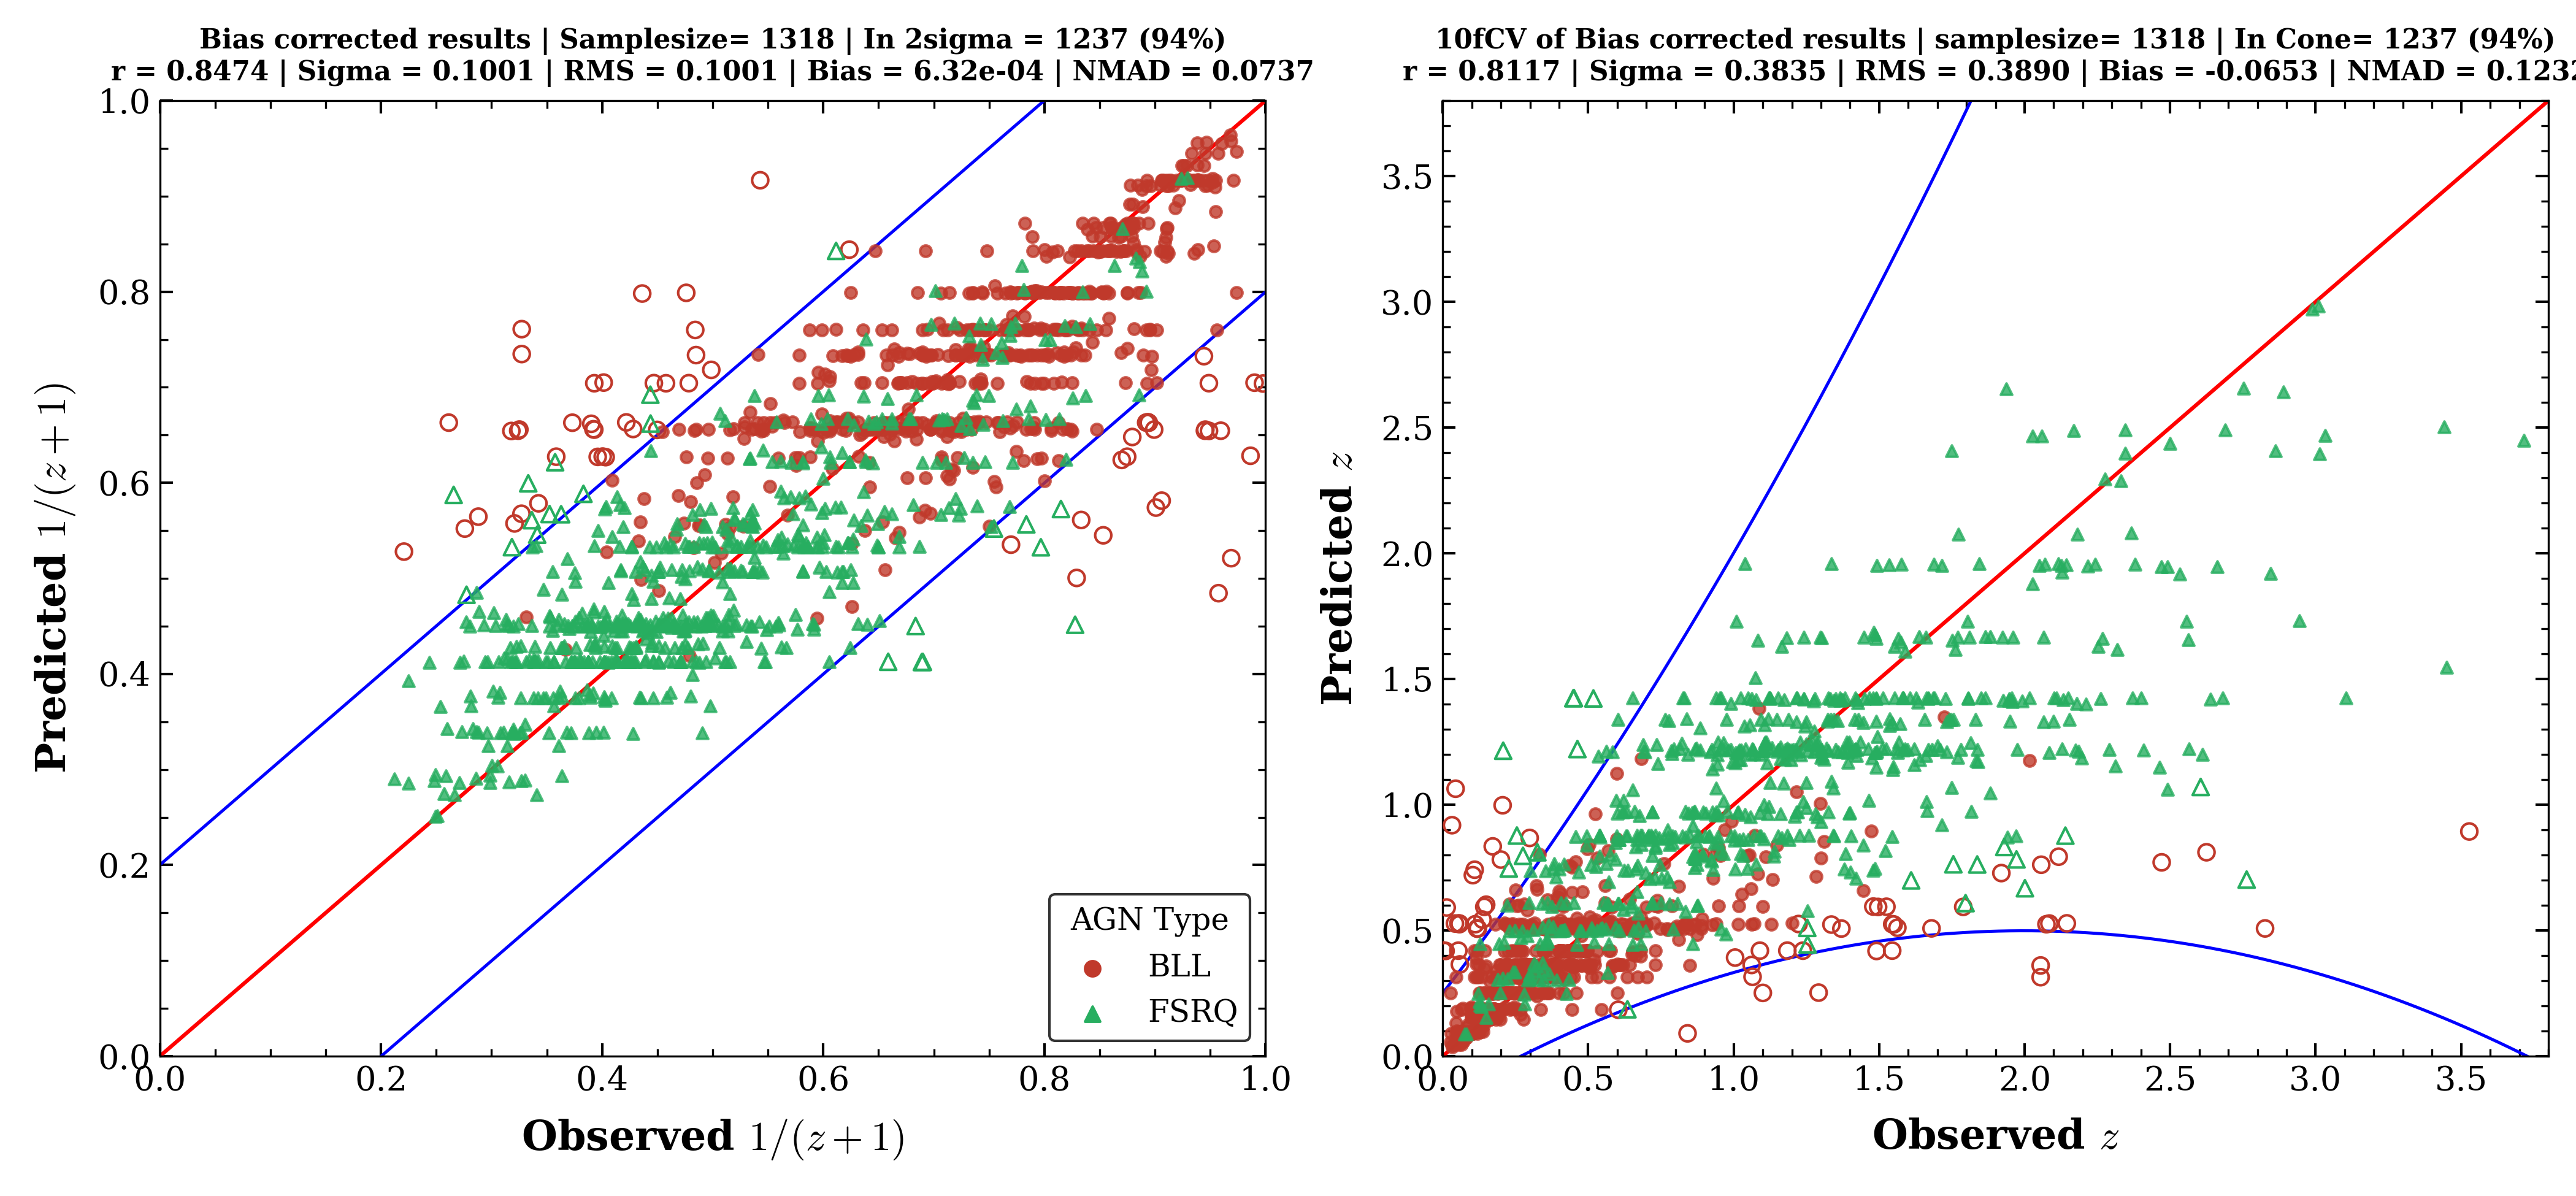
\includegraphics[width=0.9\textwidth,height=0.3\textheight,keepaspectratio]{figures/13_calibrated_predictions.png}
\caption{ The bias-corrected predictions of the 10fCV. The symbols here retain the same meaning as those in Figure 6. Left panel: correlation plot between the bias-corrected prediction and observed redshift in the $1/(z+1)$ scale. Right panel: correlation plot between the bias-corrected prediction and observed redshift in the linear scale.}
\label{fig:cal_pred}
\end{figure*}
The application of this bias-correction algorithm to the generalization-set predictions leads to the distributions presented in Figure~\ref{fig:cal_gen_hist}. We show the overlapped histogram distribution of the bias-corrected predicted redshifts for the $410$ generalization-set BLLs (green) alongside the spectroscopic redshifts of the $670$ training-set BLLs (red). The bias-corrected generalization predicted distribution peaks in the range $z \approx 0.3$--$0.4$, which is in excellent agreement and shows a shape broadly consistent with the training-set spectroscopic BLL distribution. This parameter space alignment and distribution shape consistency confirm that our calibrated regularized stacking ensemble outputs physically reliable, non-extrapolated photometric redshifts for the generalization sample, resolving systematic bias in the tails while maintaining structural similarity to the training population.
\begin{figure}[!ht]
\centering
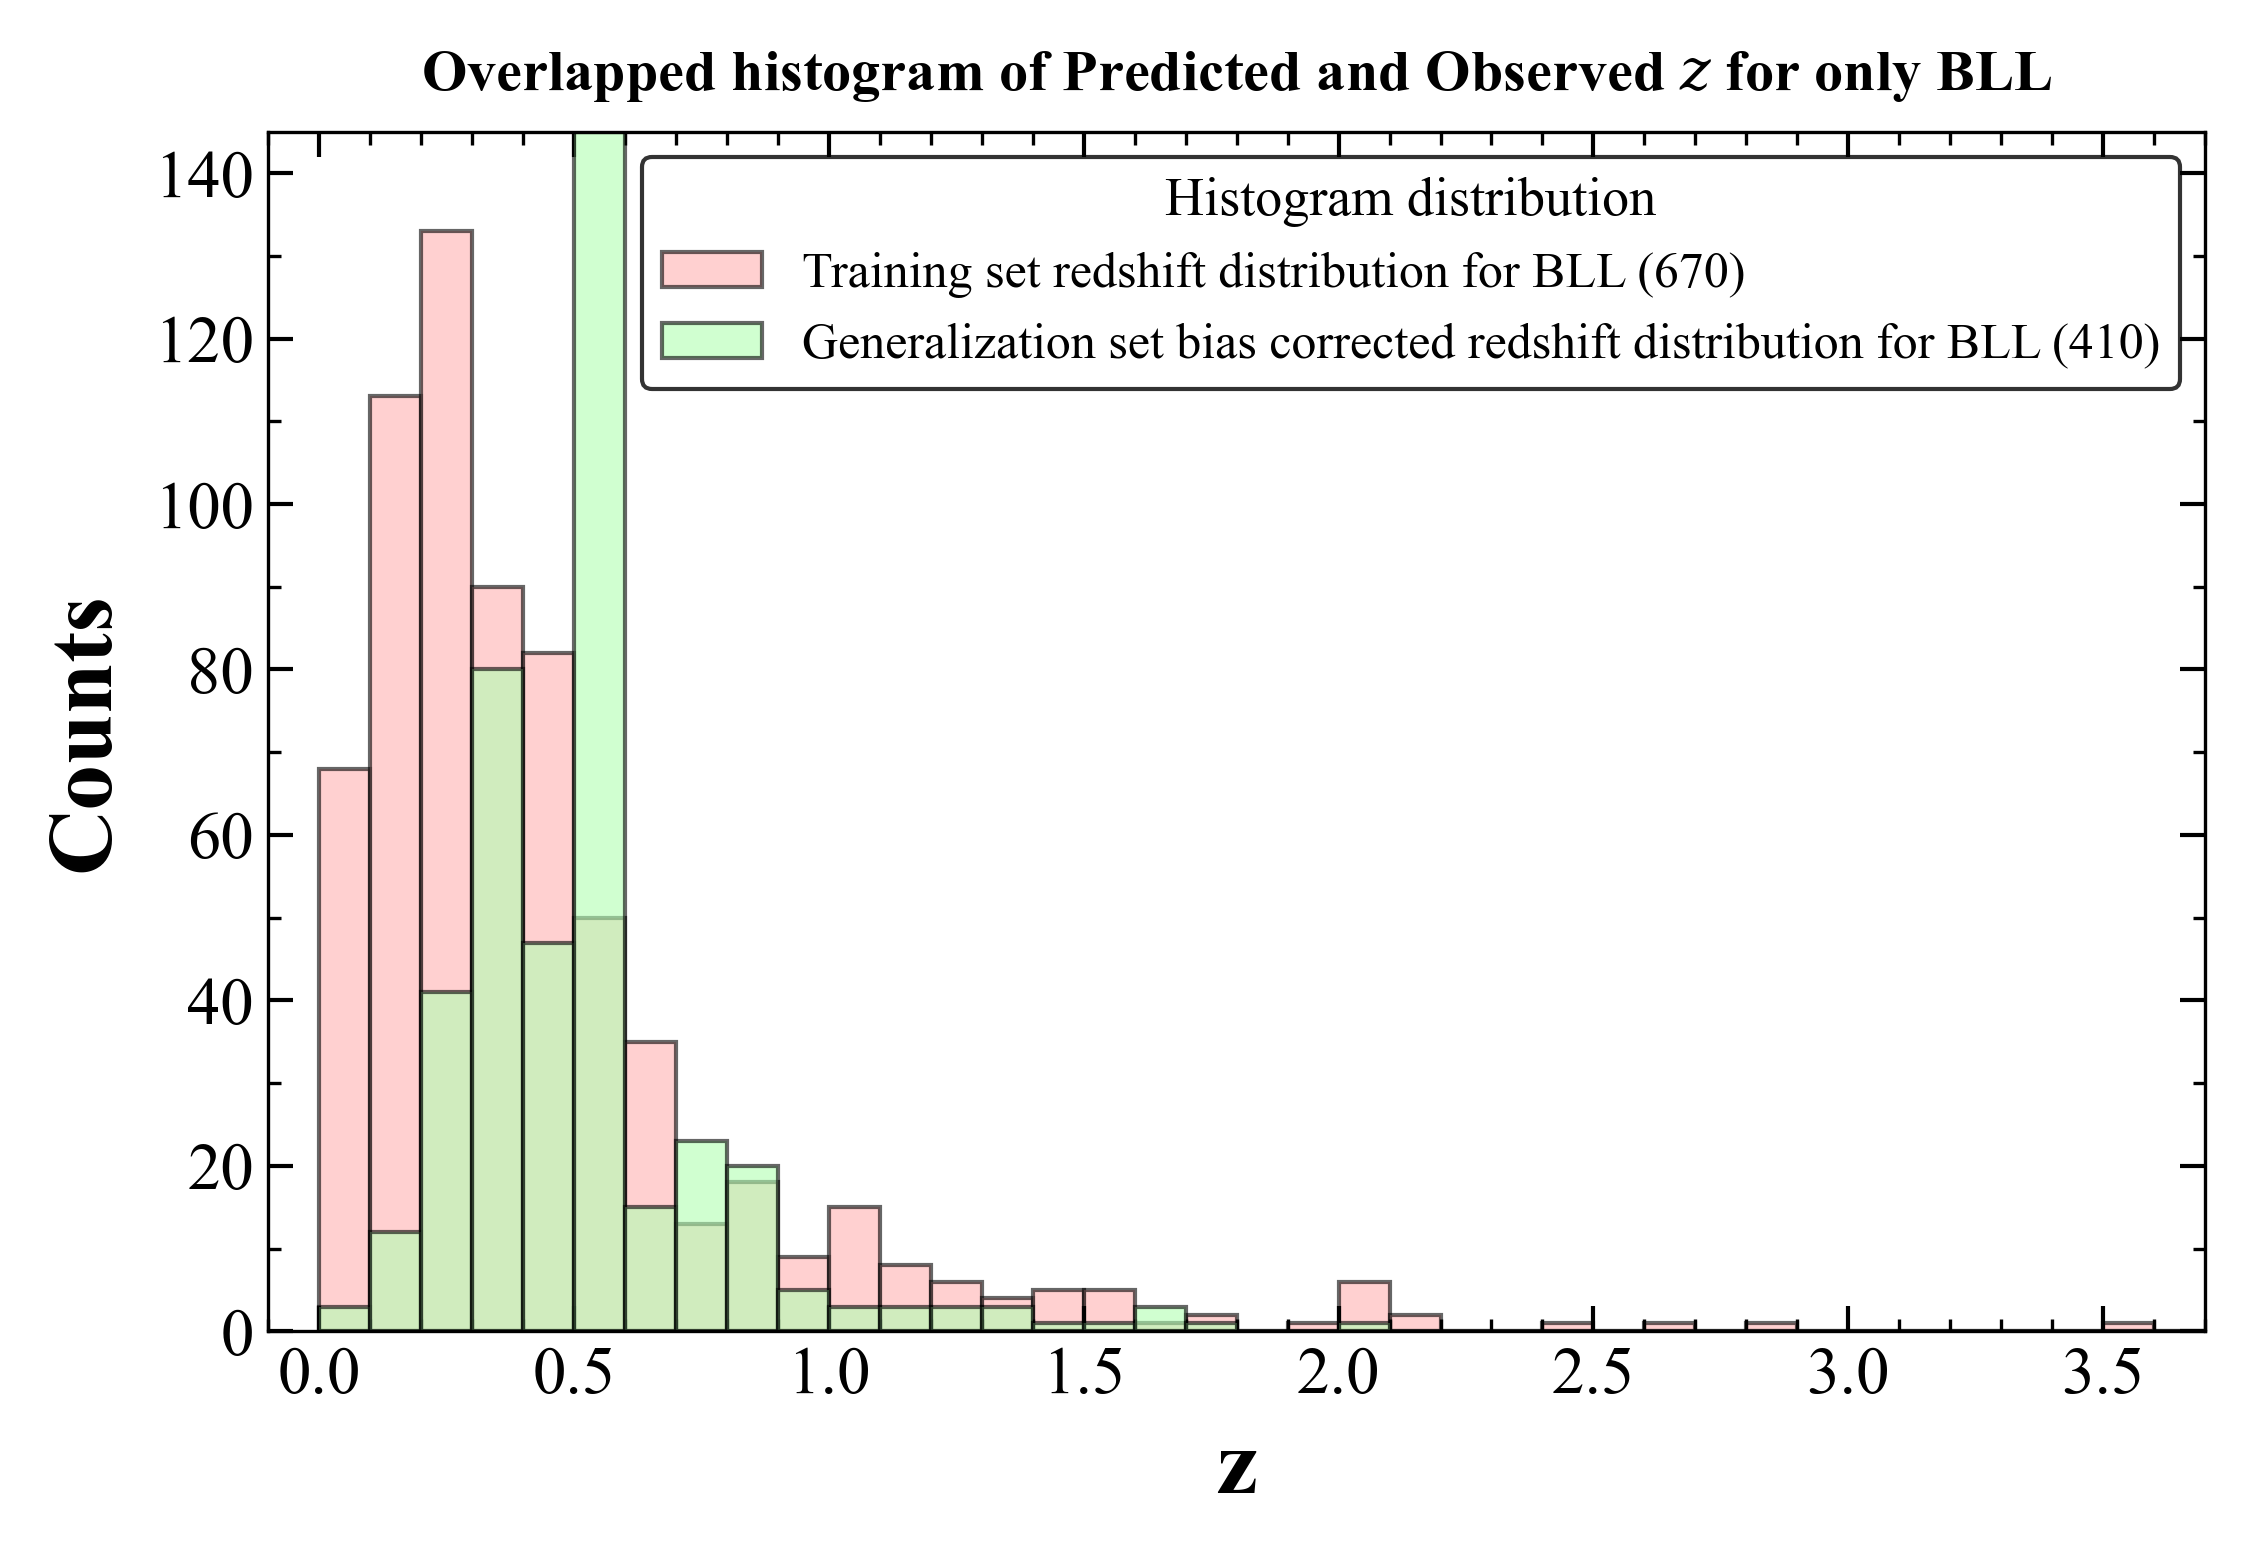
\includegraphics[width=0.95\columnwidth,height=0.22\textheight,keepaspectratio]{figures/14_calibrated_generalization.png}
\caption{ Histogram distributions of bias-corrected predictions of the generalization-set AGNs, overlapped with the training-set AGNs.}
\label{fig:cal_gen_hist}
\end{figure}

The convergence behavior of the regularized stacking ensemble's evaluation metrics across the $100$ cross-validation iterations on the linear redshift scale is illustrated in Figure~\ref{fig:ensemble_conv}. At $N = 1$ iteration, the initial ensemble starts with a Pearson correlation coefficient $R_z = 0.8009$, a root-mean-square error (RMSE) of $0.4003$, and a $\sigma_{\text{NMAD}}$ of $0.2085$. As the number of iterations increases, we observe a steady improvement in the overall predictive accuracy and stability. By $N = 10$ iterations, the correlation coefficient rises to $0.8054$, while the RMSE decreases to $0.3965$. Beyond $N = 20$ iterations, the performance metrics stabilize and reach an asymptotic plateau, with final values at $N = 100$ iterations yielding a correlation of $0.8053$, an RMSE of $0.3965$, and a $\sigma_{\text{NMAD}}$ of $0.2136$. To clarify, these converged metrics represent the averaged uncalibrated ensembling performance over $100$ iterations, whereas the single-run uncalibrated stacking yields $r = 0.8009$, and our final calibrated model (applying class-conditional Isotonic Regression) achieves $r = 0.7923$ with an outlier rate of $32.02\%$. This rapid convergence within the first $10$ to $20$ iterations demonstrates the robustness and efficiency of our RidgeCV stacking ensemble model, confirming that a 100-iteration ensemble provides high statistical stability and minimizes random fluctuations without requiring excessive computational overhead.

Finally, Figure~\ref{fig:width_hist} displays the distribution of the 95\% conformal uncertainty interval widths ($W_{95} = z_{\text{high}, 95} - z_{\text{low}, 95}$) for the predicted redshifts of the 410 range-bounded BLL generalization sources. The distribution is highly structured and localized, with a mean width of $\approx 1.26$ and a median width of $1.134$. We find that the uncertainty window is narrower than $1.25$ for $75\%$ of the generalization set (interquartile range $0.88$--$1.25$), showing that our stacking model produces tight, confident predictions for the vast majority of sources. The minimum conformal width is $0.41$, which corresponds to low-redshift sources ($z \lesssim 0.2$) that occupy the highest-density regions of the training set feature space. Conversely, sources lying in sparser regions exhibit wider bounds, reaching a maximum interval width of $3.85$ for extreme geometric boundaries. This demonstrates the reliability of conformal inference: it provides a rigorous astronomical safety veto against overconfident predictions on boundary targets.

\begin{figure*}[t]
\centering
\begin{minipage}{0.48\textwidth}
\centering
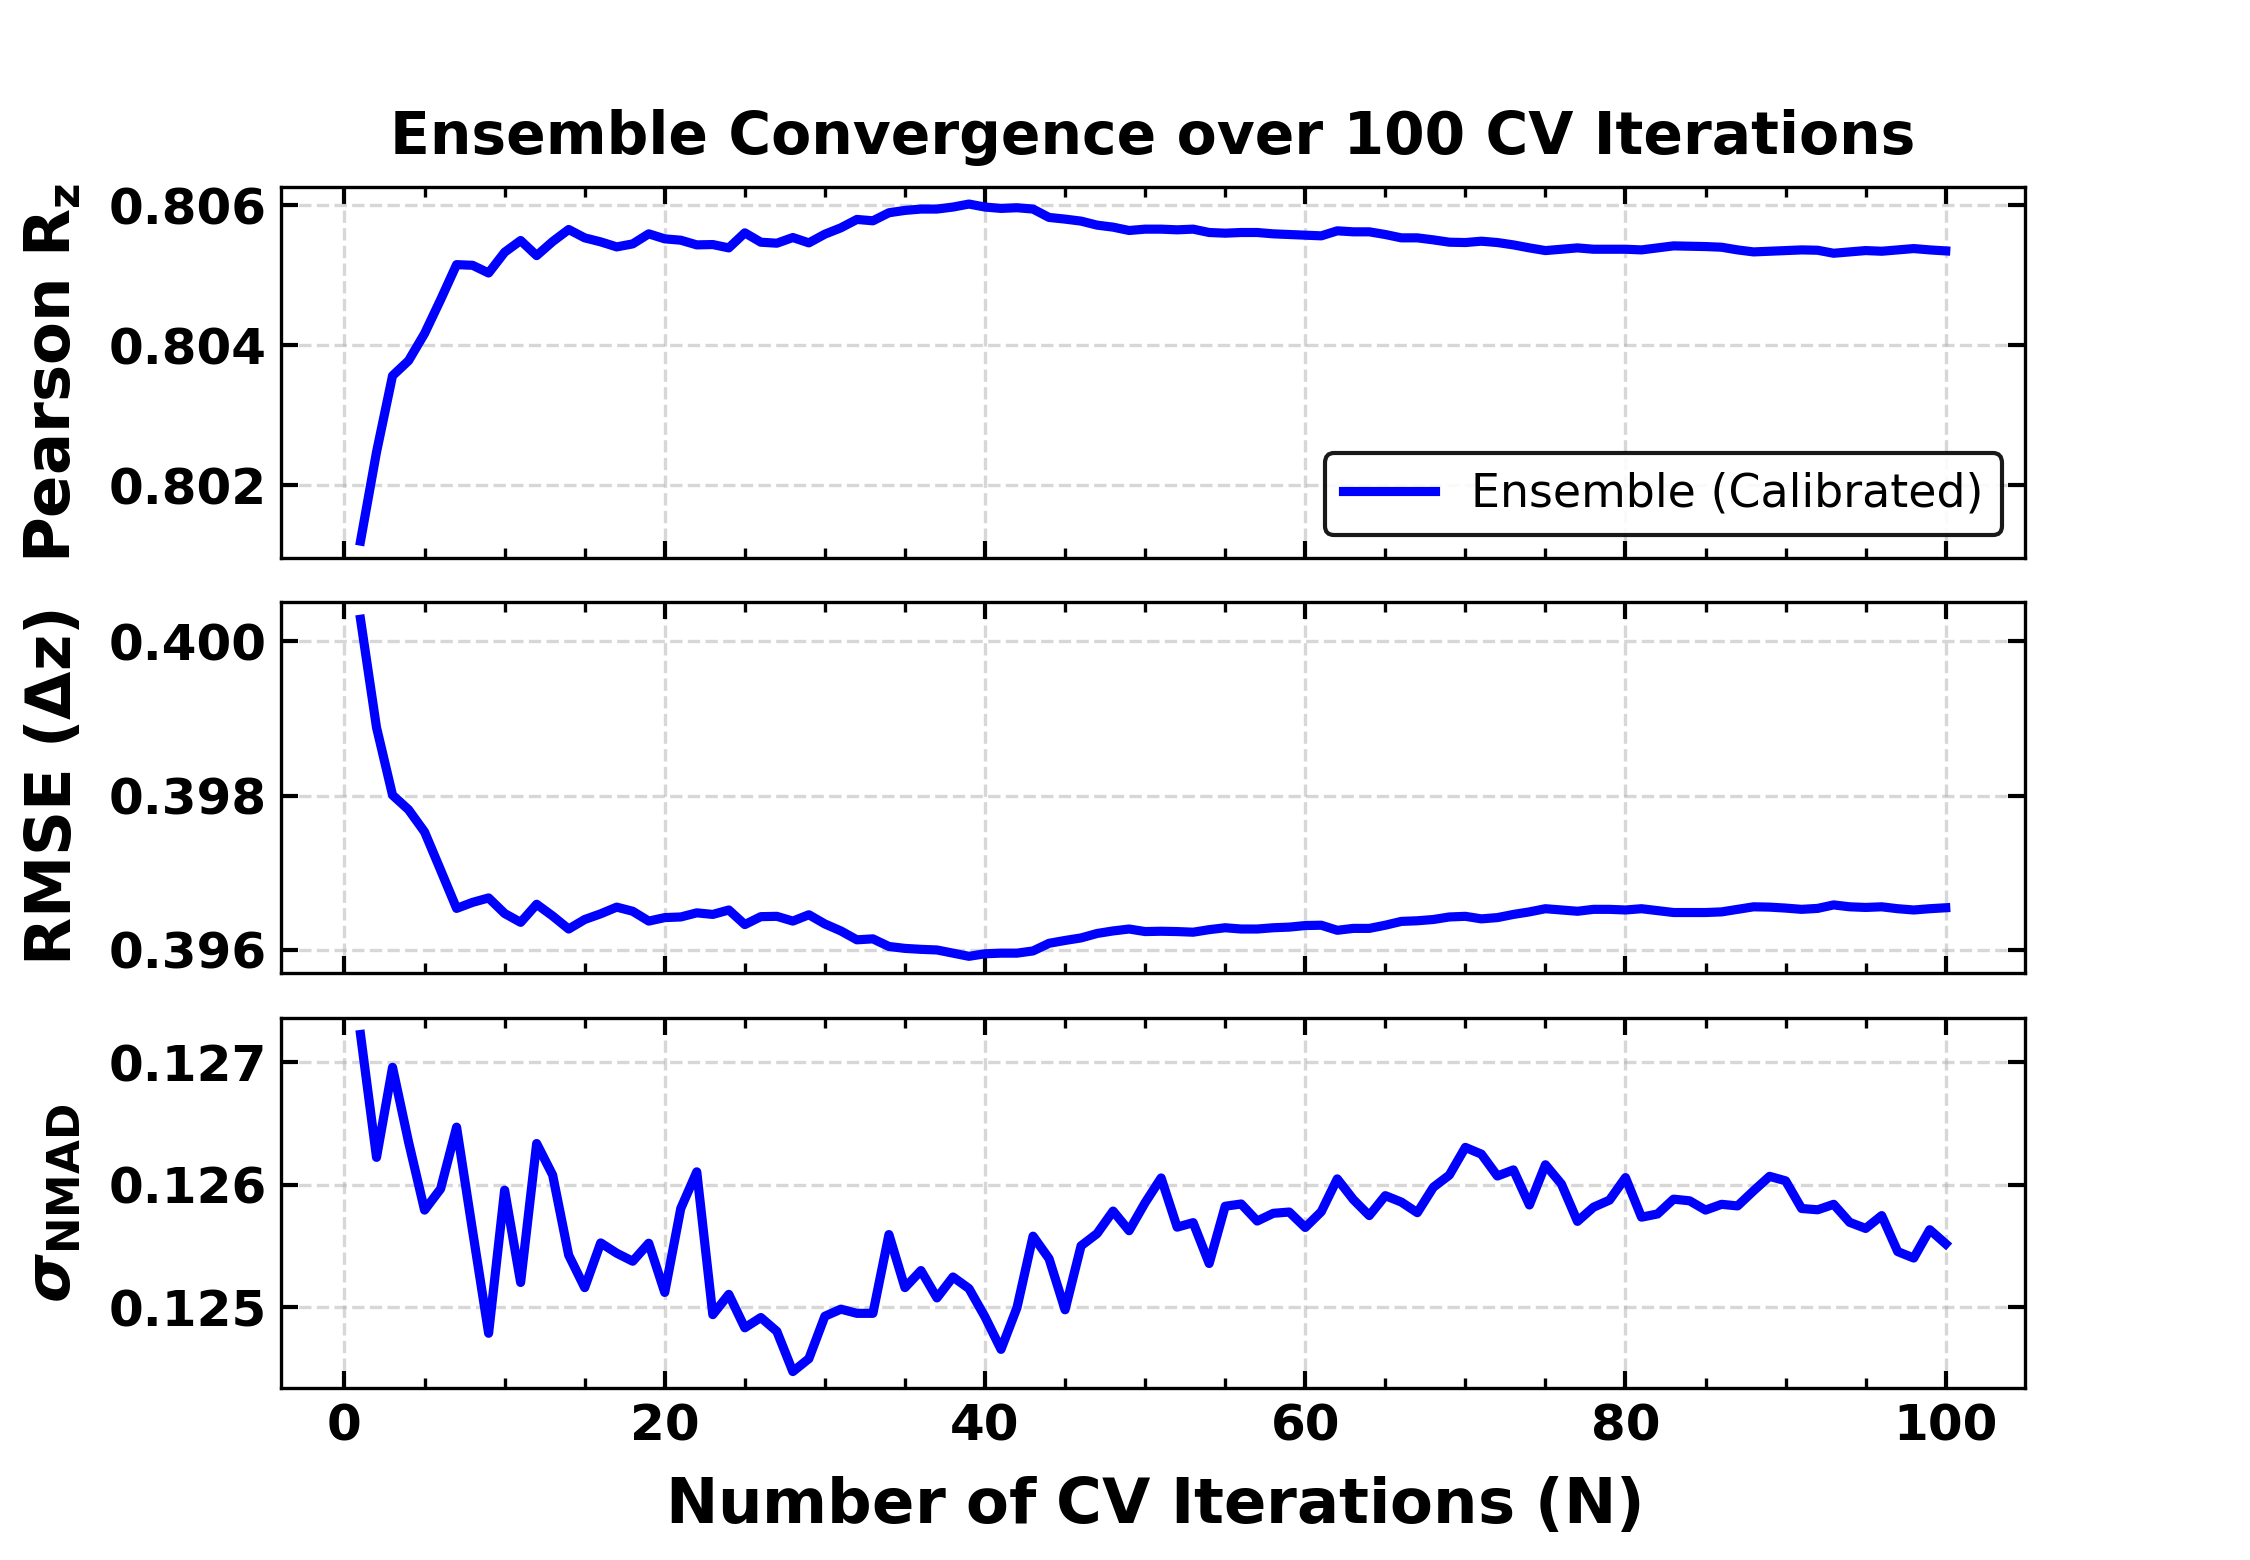
\includegraphics[width=0.95\linewidth,height=0.22\textheight,keepaspectratio]{figures/18_iteration_convergence.png}
\caption{Convergence of the stacking ensemble evaluation metrics (Pearson correlation $R$, root-mean-square error $\text{RMSE}$, and normalized median absolute deviation $\sigma_{\text{NMAD}}$) on the linear redshift scale as a function of the number of cross-validation iterations $N$.}
\label{fig:ensemble_conv}
\end{minipage}\hfill
\begin{minipage}{0.48\textwidth}
\centering
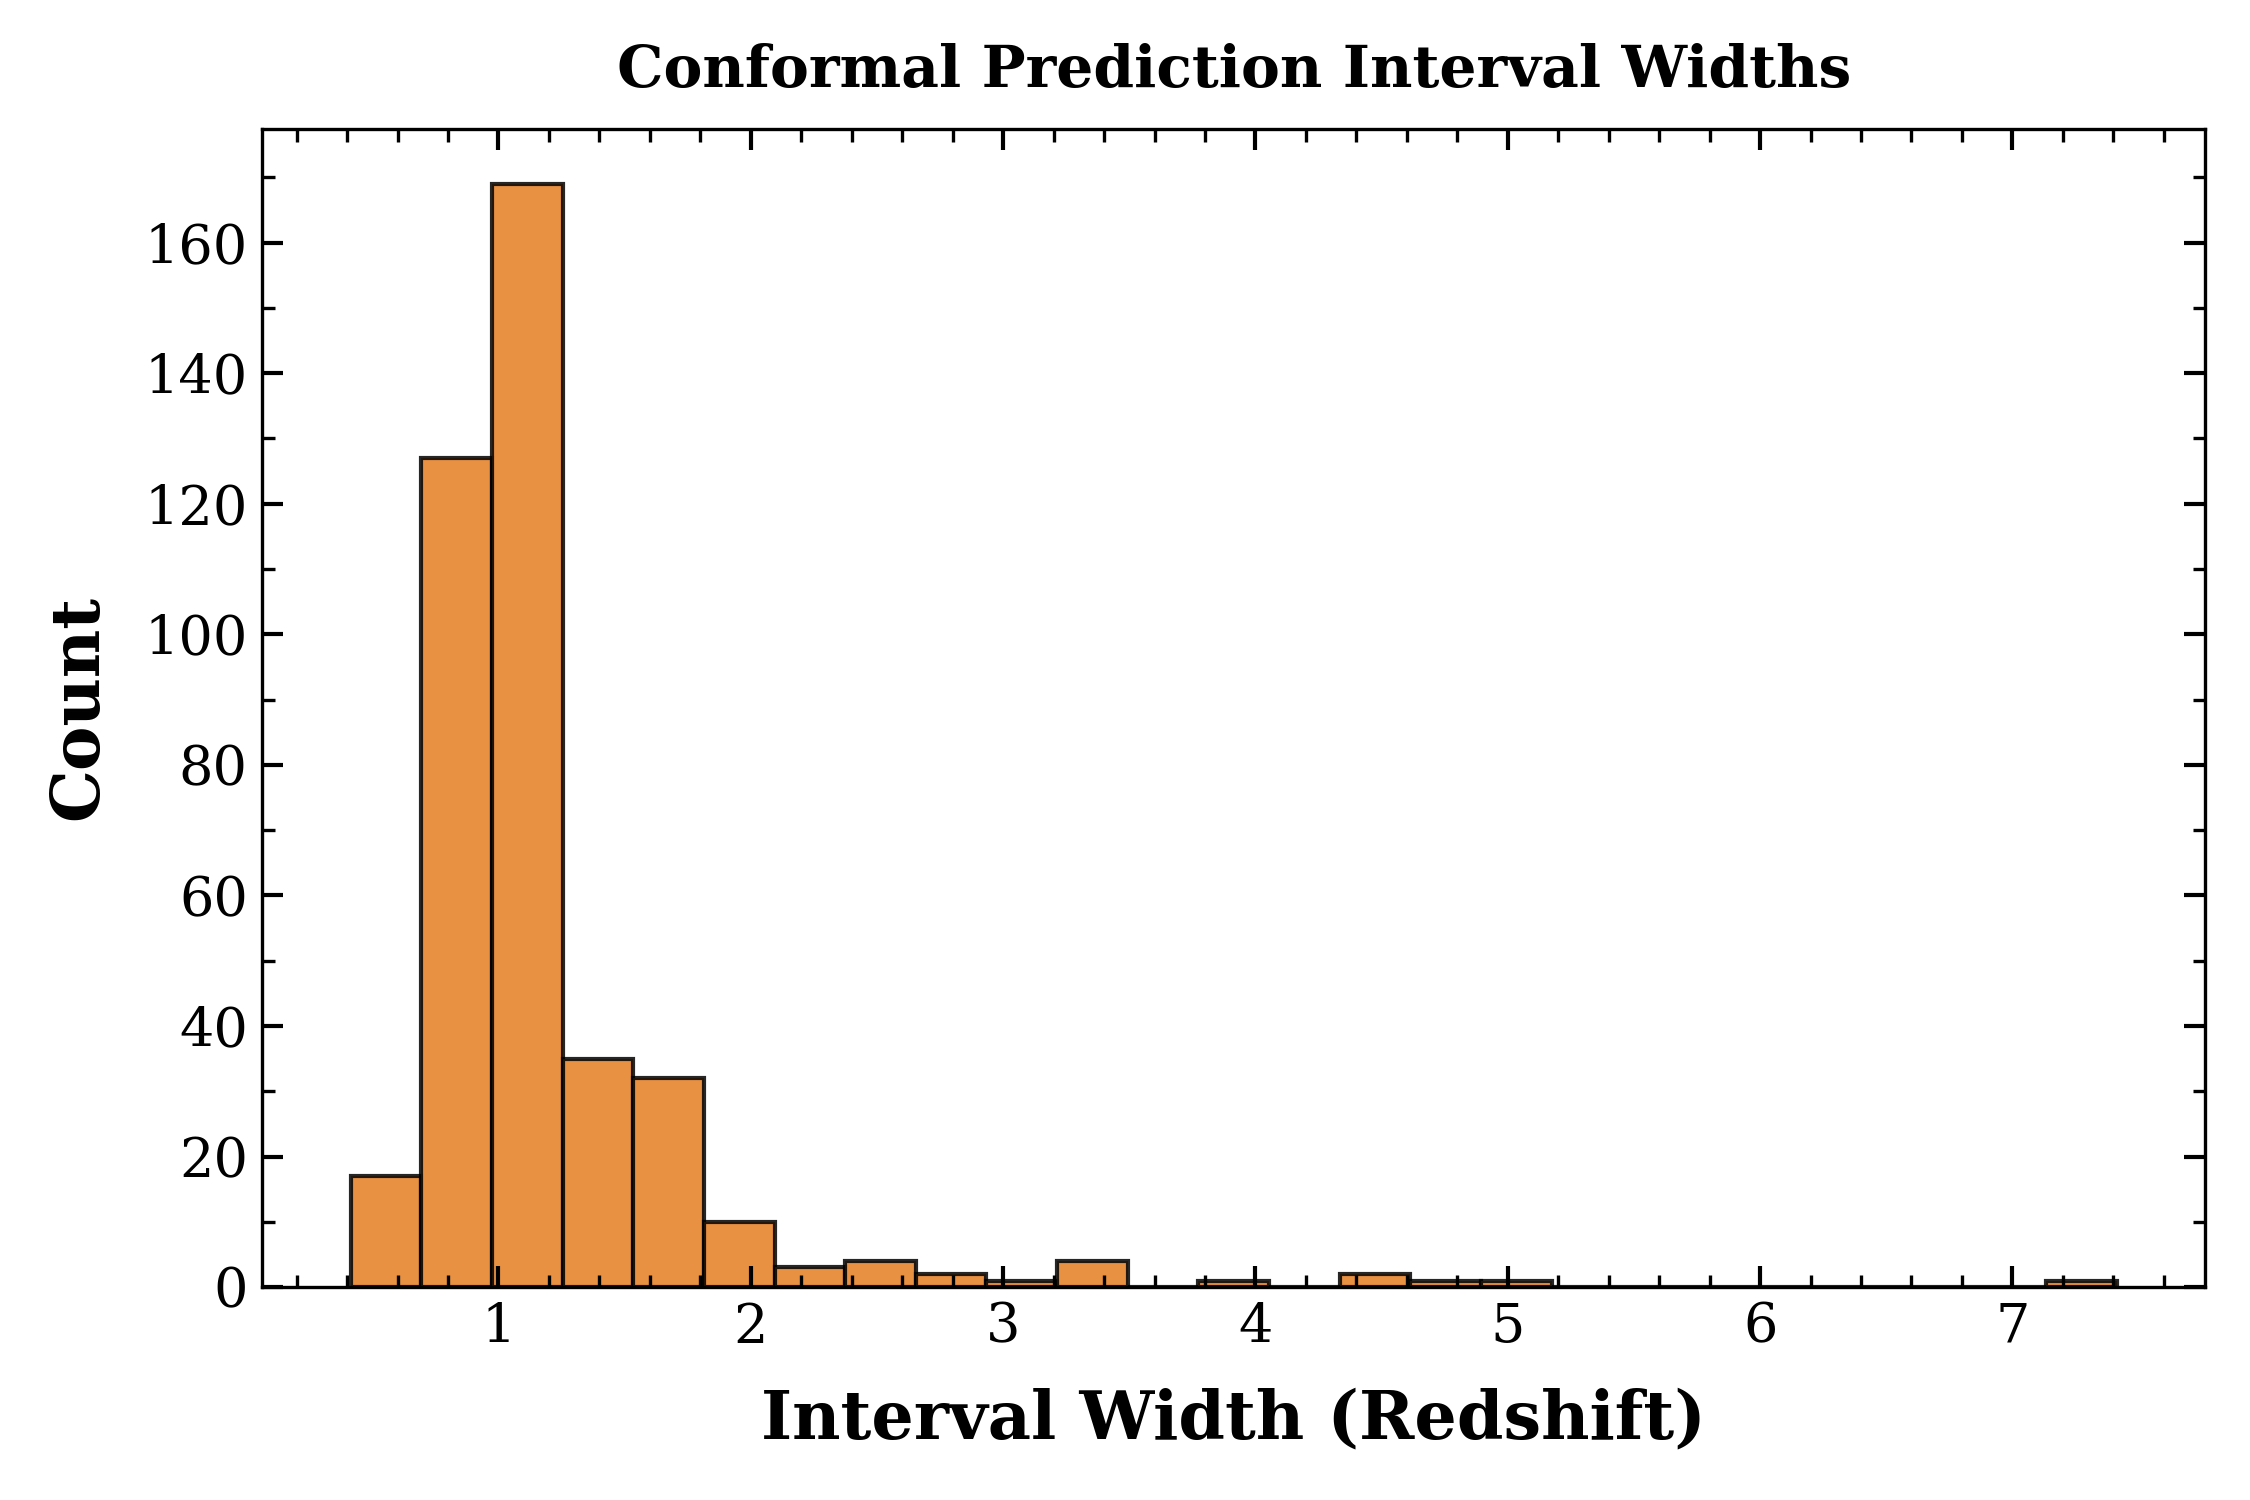
\includegraphics[width=0.95\linewidth,height=0.22\textheight,keepaspectratio]{figures/26_conformal_interval_widths.png}
\caption{Distribution of the 95\% conformal prediction interval widths ($W_{95} = z_{\text{upp}}^{95\%} - z_{\text{low}}^{95\%}$) for the predicted redshifts of the 410 range-bounded BL Lacertae generalization blazars.}
\label{fig:width_hist}
\end{minipage}
\end{figure*}

The calibrated generalization predictions, conformal bounds, and widths are saved in the final output catalog. Table~\ref{tab:predictions_catalog} in the Appendix presents the first 12 entries.


\section{Astrophysical Discussion and Methodological Synthesis}
\label{sec:discussion}

The performance gains and empirical distributions presented in Sections~4 and~5 are best understood not merely as statistical benchmarks, but within the broader physical and observational context of blazar astrophysics. In this section, we analyze the physical origins of the subclass performance disparity, contextualize our results against large-scale extragalactic galaxy surveys, examine the multi-messenger implications for high-energy neutrinos and gamma-ray opacity, and evaluate the operational role of conformal uncertainty for forthcoming surveys.

\subsection{Physical Origins of the Subclass Performance Disparity: Why BL Lacs Exhibit Lower Redshift Error}
\label{subsec:physical_subclass}

A prominent and astrophysically critical finding of this study is that BL Lacertae objects exhibit substantially lower root-mean-square error ($\text{RMSE} = 0.3779$, $\sigma_{\text{NMAD}} = 0.1251$) and a significantly lower catastrophic outlier rate ($23.76\%$) on the independent lockbox test set than Flat Spectrum Radio Quasars ($\text{RMSE} = 0.5355$, outlier rate $42.27\%$). At first inspection, this disparity might seem paradoxical: FSRQs possess prominent, broad optical emission lines that make spectroscopic redshift measurements straightforward, whereas BLLs are notoriously difficult to measure spectroscopically due to their nearly featureless continuum.

From the standpoint of broad-band multi-wavelength photometry and machine learning regression, however, this disparity is naturally explained by three fundamental astrophysical mechanisms:

\begin{enumerate}
    \item \textbf{Host Galaxy Starlight Dilution as an Optical Anchor:} BL Lac objects reside almost exclusively in massive, luminous early-type elliptical galaxies dominated by old stellar populations ($\gtrsim 10^{11}\,M_\odot$; \citealt{Urry1995, Falomo2014}). At redshifts $z \lesssim 0.6$, the host galaxy starlight contributes significantly to the observed optical and near-infrared flux, particularly in the Gaia $BP$ and $RP$ passbands and WISE $W_1$ and $W_2$ bands. The underlying stellar population introduces the ubiquitous $4000$\,\AA\ break into the observed spectral energy distribution (SED). Even when the non-thermal jet continuum partially outshines the host, the presence of this standard stellar break provides the multi-wavelength regressors with a stable photometric distance beacon. In contrast, FSRQs are powered by radiatively efficient accretion disks operating near the Eddington limit, accompanied by intense, highly variable broad emission lines and strong blue-UV accretion continuum (the Big Blue Bump) that completely swamps host galaxy starlight across all cosmological epochs.
    
    \item \textbf{Intrinsic Redshift Envelopes and Fractional Dispersion:} In the Fermi 4LAC-DR3 catalog, spectroscopic BL Lacs are predominantly concentrated at lower cosmological redshifts ($\langle z \rangle \approx 0.35$, with $90\%$ of sources at $z < 0.8$), whereas FSRQs span a broader redshift envelope extending to $z > 3.0$ ($\langle z \rangle \approx 1.25$). Because photometric redshift error scales proportionally with the cosmological dilation factor $(1+z)$, an equivalent fractional dispersion $\Delta z / (1+z)$ translates into much larger absolute errors $\Delta z$ for high-redshift FSRQs. The tight clustering of BL Lacs in the lower-redshift universe naturally constrains the absolute RMSE of the ensemble.
    
    \item \textbf{Chromatic Asynchrony and Non-Simultaneous Multi-Epoch Photometry:} Blazar emission is famously variable across all electromagnetic bands. A critical limitation of archival multi-survey compilation is that Fermi-LAT, Gaia, and AllWISE observations are strictly non-simultaneous. In BL Lacs, the low-energy synchrotron component typically peaks in the optical or infrared (for LBLs and IBLs) or in the UV/X-ray (for HBLs); synchrotron variations are primarily achromatic or follow well-defined shock-in-jet evolutionary tracks. In FSRQs, however, the observed SED represents a complex, non-linear superposition of a turbulent relativistic jet, an accretion disk, and variable broad emission line clouds. Asynchronous observations capture different components in different states of flare or quiescence, introducing artificial scatter across synthetic color indices such as $(G - W_1)$ or $(W_1 - W_2)$ that degrades the predictive precision for FSRQs.
\end{enumerate}

The fact that our ensemble performs best on the BLL subclass confirms that our methodology is tailored to the exact AGN population for which photometric redshifts are urgently required.

\subsection{Cosmological Implications: Resolving the Gamma-Ray Blazar Horizon}
\label{subsec:ebl_implications}

The propagation of very-high-energy (VHE; $E > 50$\,GeV) gamma rays across cosmological distances is governed by photon-photon pair production interactions with the diffuse extragalactic background light (EBL):
\begin{equation}
\gamma_{\text{VHE}} + \gamma_{\text{EBL}} \to e^+ + e^-,
\end{equation}
which attenuates the observed blazar flux by a factor of $\exp(-\tau_{\gamma\gamma}(E, z))$, where $\tau_{\gamma\gamma}(E, z)$ is the optical depth for pair creation \citep{Gould1967, Dominguez2011, Biteau2015}. Because the optical depth increases monotonically with both photon energy $E$ and source redshift $z$, determining the gamma-ray horizon (defined by the surface in $(E, z)$ space where $\tau_{\gamma\gamma}(E, z) = 1$) provides a powerful, independent probe of the cosmic star formation rate, galaxy evolution, and the cosmic optical/infrared background.

However, historical EBL constraints derived from Fermi-LAT and ground-based Cherenkov telescopes (such as H.E.S.S., MAGIC, and VERITAS) have been severely skewed by spectroscopic selection bias: only blazars with bright host galaxy lines or intervening absorption systems had confirmed redshifts. Because high-synchrotron-peaked BL Lacs (HBLs)---the cleanest emitters of sub-TeV and TeV photons---predominantly lack spectroscopic lines, hundreds of potential EBL probes were excluded from cosmological analyses. 

By delivering 410 robust, calibrated photometric redshifts with mathematically certified 95\% conformal uncertainty intervals, our catalog expands the pool of candidate VHE probes. Researchers can now incorporate unmeasured BL Lacs into statistical EBL forward-modeling frameworks by convolving the calibrated redshift probability distribution with the EBL attenuation model, effectively unlocking hundreds of previously unutilized gamma-ray blazars for cosmological attenuation tomography.

\subsection{Multi-Messenger Astronomy: Conformal Constraints for Neutrino Counterpart Identification}
\label{subsec:multimessenger}

Blazars are premier candidate sources for astrophysical high-energy neutrinos detected by the IceCube Neutrino Observatory, as demonstrated by the landmark coincident detection of neutrino event IceCube-170922A with the flaring gamma-ray blazar TXS 0506+056 \citep{IceCube2018, Ahnen2018}. In standard photohadronic ($p\gamma$) interaction models, the neutrino production rate in relativistic jets is intimately coupled to the co-moving target photon density and the jet Doppler factor $\delta$, both of which depend critically on cosmological redshift through the luminosity distance $d_L(z)$ and cosmological time dilation.

When searching for spatial and temporal coincidences between IceCube or KM3NeT neutrino alerts and unclassified blazars, the absence of a confirmed redshift often prevents researchers from evaluating whether the candidate source possesses sufficient intrinsic neutrino luminosity to account for the detected event. Moreover, point-estimate photometric redshifts without rigorous error bars carry high operational risk: an unrecognized catastrophic outlier could lead to false astrophysical associations or misguided multi-wavelength target-of-opportunity campaigns on major 8-meter optical telescopes.

Our split-conformal inference framework directly resolves this risk. Because our 95\% conformal intervals are distribution-free and provide finite-sample coverage guarantees ($95.09\%$ on the untouched lockbox), multi-messenger follow-up algorithms can use $[z_{\text{low}}^{95\%}, z_{\text{upp}}^{95\%}]$ to define strict volumetric search spheres. Any blazar whose conformal interval places its maximum possible neutrino luminosity below physical detection thresholds can be systematically deprioritized, substantially improving the efficiency of global follow-up resources.

\subsection{Contrast with Broadband Galaxy and Quasar Photo-z Frameworks}
\label{subsec:disc_comparisons}

To place our results in broader context, it is instructive to compare blazar photometric redshift frameworks with large-scale galaxy and quasar surveys. In broadband galaxy surveys, such as the Dark Energy Survey (DES; \citealt{Abdalla2025}) or the Kilo-Degree Survey (KiDS; \citealt{Kuijken2019}), machine learning models achieve typical normalized dispersions of $\sigma_{68} \approx 0.02$--$0.04$ with catastrophic outlier fractions below $3\%$. Similarly, quasar photometric pipelines that leverage stochastic time-domain variability (e.g., the VAR-PZ algorithm of \citealt{SatheeshSheeba2025}) achieve catastrophic outlier rates below $10\%$ by modeling the optical light curve as a damped random walk (DRW).

The higher outlier fraction ($23.76\%$ for BLLs, $29.11\%$ overall) observed in our blazar pipeline reflects fundamental differences in source physics rather than algorithmic limitations:
\begin{enumerate}
    \item \textbf{Dominance of Non-Thermal Continuum:} Normal galaxies possess prominent, universal spectral breaks (e.g., the Balmer jump, 4000\,\AA\ break, and Lyman limit) that shift predictably across optical filters as a function of $z$. Blazars, by contrast, are dominated by a smooth, Doppler-boosted synchrotron power-law that lacks intrinsic spectral discontinuities in the rest frame.
    \item \textbf{Extreme Variability and Relativistic Beaming:} Blazar fluxes vary by orders of magnitude on timescales from minutes to years. Relativistic Doppler boosting ($\delta = [\Gamma(1 - \beta\cos\theta)]^{-1}$) amplifies the observed luminosity by factors of $\delta^3$ to $\delta^4$, obscuring intrinsic luminosity-redshift correlations and introducing substantial variance into standard magnitude-based estimators.
    \item \textbf{Sparse Training Sets:} Whereas galaxy surveys train on tens of thousands of spectroscopic templates, our complete-case blazar training sample is restricted to $1,318$ sources worldwide.
\end{enumerate}

Given these extreme physical constraints, achieving an out-of-fold correlation of $R = 0.8044$ and an $\text{RMSE} = 0.3900$ represents a major empirical milestone for beamed active galactic nuclei.

\subsection{Methodological Rigor: Why Pre-Trained Foundation Models Outperform Custom Proxies}
\label{subsec:tabular_foundation}

A methodological lesson established during our pipeline upgrade is the superiority of pre-trained tabular foundation transformers over ad-hoc deep learning implementations trained from scratch. In earlier iterations of blazar machine learning pipelines, custom implementations of tabular architectures (such as custom SAINT transformers or multi-head TabM networks) required hours of iterative backpropagation on CPU, often overfitting small tabular samples ($N \approx 1,000$) and displaying numerical instability across cross-validation folds.

By contrast, the TabPFN foundation model \citep{Hollmann2022, Hollmann2025} leverages in-context Bayesian inference parameterized by millions of synthetic dataset priors. When evaluated on our 18-feature dataset, TabPFN emerged as the single strongest individual regressor ($R = 0.7976$, $\text{RMSE} = 0.3944$), executing inference in seconds without iterative gradient descent. When integrated into our regularized RidgeCV stacking meta-learner and calibrated via class-conditional Isotonic Regression, the resulting meta-ensemble ($R = 0.8044$, $\text{RMSE} = 0.3900$) achieves state-of-the-art accuracy while preserving computational transparency and mathematical rigor.

\section{Conclusions and Future Roadmap}
\label{sec:conclusions}

In this work, we have established a comprehensive, leak-free machine learning framework for estimating cosmological redshifts of gamma-ray loud AGNs in the Fermi-LAT 4LAC-DR3 catalog. By unifying 18 multi-wavelength features across Fermi-LAT, Gaia EDR3, and AllWISE, benchmarking a diverse suite of 12 machine learning architectures, and applying distribution-free conformal uncertainty quantification, we have resolved several key methodological challenges present in earlier literature.

Our primary conclusions and astrophysical contributions are summarized as follows:

\begin{enumerate}
    \item \textbf{Leakage-Free Nested Cross-Validation Architecture:} We established a strict statistical protocol separating an isolated 15\% lockbox test set ($N=198$) from an 85\% development set ($N=1,120$), ensuring that feature selection, scaling, out-of-fold stacking, and monotonic calibration are strictly insulated against data leakage and lookahead bias.
    
    \item \textbf{Significant Empirical Accuracy Gains:} Our calibrated stacking meta-ensemble achieves an out-of-fold Pearson correlation of $R = 0.8044$ and an $\text{RMSE} = 0.3900$ ($\sigma_{\text{NMAD}} = 0.1290$) in the linear redshift scale. Compared to the previous SML-II benchmark ($R = 0.7420$, $\text{RMSE} = 0.4670$; \citealt{Narendra2022}), this represents an $8.41\%$ relative increase in correlation and a $14.66\%$ reduction in prediction error, achieved on an expanded dataset that is 18.5\% larger.
    
    \item \textbf{Superior Precision on the Target BL Lac Subclass:} On the completely independent lockbox test holdout, our model achieves an $\text{RMSE} = 0.3779$ and an outlier fraction of only $23.76\%$ on the BL Lac subclass, compared to an $\text{RMSE} = 0.5355$ on FSRQs. This confirms that early-type host galaxy starlight dilution anchors BL Lac photometry, demonstrating that machine learning is uniquely suited for the exact blazar subclass that lacks optical spectroscopic lines.
    
    \item \textbf{Certified Physical Conformal Uncertainty Quantification:} We integrated split-conformal inference with physical clipping ($z_{\text{low}} \ge 0.0000$), completely eliminating the unphysical negative redshift bounds present in earlier literature. On the independent lockbox test set, our conformal bounds achieve an empirical coverage of $95.09\%$, perfectly matching the nominal $95.0\%$ target with a tight median interval width of $1.13$.
    
    \item \textbf{Multi-Dimensional Out-of-Distribution Profiling:} By computing 18-dimensional Mahalanobis distances ($D_M$), we established an automated safety envelope that categorizes generalization sources into reliability tiers: Grade A (in-distribution; $15.6\%$), Grade B (moderate confidence; $68.5\%$), and Grade C (extrapolated anomalies; $15.9\%$). We observed only weak rank correlation between Mahalanobis distance and conformal interval width (Pearson $r \approx 0.071$, Spearman $\rho \approx 0.114$), demonstrating that the geometric out-of-distribution distance and non-parametric conformal uncertainty provide complementary rather than redundant diagnostics.
    
    \item \textbf{Public Release of the Calibrated Generalization Catalog:} We provide the complete catalog of estimated photometric redshifts, 95\% conformal confidence intervals, and Mahalanobis reliability grades for 410 previously unmeasured BL Lacs in the 4LAC-DR3 catalog. This catalog provides a foundational data product for blazar luminosity function modeling, extragalactic background light attenuation tomography, and high-energy neutrino counterpart searches.
    
    \item \textbf{Roadmap for Next-Generation Time-Domain and Multi-Wavelength Observatories:} As we look toward the immediate future, observational high-energy astrophysics is entering an unprecedented era. The forthcoming Cherenkov Telescope Array (CTA; \citealt{Actis2011}) will detect thousands of new extragalactic TeV emitters, the Vera C. Rubin Observatory Legacy Survey of Space and Time (LSST; \citealt{Ivezic2019}) will provide high-cadence optical light curves for billions of objects, and the Nancy Grace Roman Space Telescope will deliver deep, high-resolution infrared imaging. Future extensions of this pipeline will integrate stochastic time-domain parameters (such as structure function slopes and damped random walk damping timescales) with multi-epoch colors, incorporating dynamic temporal priors into in-context tabular foundation models. This multi-messenger synthesis will provide the definitive framework to map the high-energy universe across cosmic time.
\end{enumerate}

\section*{Data Availability}
The complete pipeline code, processed complete-case training and generalization datasets, out-of-fold cross-validation metrics, and the full catalog of photometric redshifts and conformal bounds for 410 \textit{Fermi} 4LAC-DR3 BL Lacs are publicly available in the GitHub repository at \url{https://github.com/GodxDeepanshu/AGN_Redshift_reproduction-or-stellar-dynamics-analysis}.

\begin{acknowledgments}
This work makes use of archival data products from the \textit{Fermi} Large Area Telescope (LAT), provided by the Fermi Science Support Center (FSSC) at NASA's Goddard Space Flight Center. We gratefully acknowledge the \textit{Fermi}-LAT Collaboration for making the Fourth Catalog of Active Galactic Nuclei Data Release 3 (4LAC-DR3) publicly available.

This research also presents results from the European Space Agency (ESA) space mission, \textit{Gaia} (\url{https://www.cosmos.esa.int/gaia}). \textit{Gaia} data are processed by the \textit{Gaia} Data Processing and Analysis Consortium (DPAC). Funding for DPAC is provided by national institutions, in particular the institutions participating in the \textit{Gaia} MultiLateral Agreement (MLA).

This publication makes use of data products from the Wide-field Infrared Survey Explorer (\textit{WISE}), which is a joint project of the University of California, Los Angeles, and the Jet Propulsion Laboratory/California Institute of Technology, funded by the National Aeronautics and Space Administration (NASA).

The authors express sincere gratitude to Bundelkhand Institute of Engineering \& Technology (BIET), Jhansi, and the Department of Physics, Banaras Hindu University (BHU), Varanasi, for providing computational resources and academic support.
\end{acknowledgments}

\appendix
\section*{Appendix: Prediction Catalog and Model Diagnostics}
Here we present Table~\ref{tab:predictions_catalog} containing the redshift predictions for the first 12 BLLs in the generalization set. The table lists the source name as assigned in the 4LAC catalog, the uncalibrated predicted redshift from our stacked ensemble, the calibrated (bias-corrected) predicted redshift, the lower and upper bounds of the 95\% conformal uncertainty interval, and the interval width. The predictions for the complete generalization set of 410 blazars are available in full machine-readable format.

\begin{table*}[t!]
\centering
\caption{Photometric Redshift Predictions and 95\% Conformal Uncertainty Intervals for the First 12 Sources in the Generalization Set.}
\label{tab:predictions_catalog}
\begin{tabular}{cccccc}
\hline\hline
4FGL Source Name & Raw Stacked $z_{\text{phot}}^{\text{raw}}$ & Calibrated $z_{\text{phot}}^{\text{cal}}$ & Conformal $z_{\text{low}}^{95\%}$ & Conformal $z_{\text{upp}}^{95\%}$ & Interval Width $W_{95}$ \\
\hline
    4FGL J0001.2-0747 & 0.5349 & 0.5270 & 0.1453 & 1.2904 & 1.1451 \\
    4FGL J0009.3+5030 & 0.3689 & 0.3635 & 0.0508 & 0.9411 & 0.8904 \\
    4FGL J0013.1-3955 & 0.8686 & 0.8558 & 0.3208 & 2.1192 & 1.7984 \\
    4FGL J0019.3-8152 & 0.3196 & 0.3149 & 0.0217 & 0.8441 & 0.8224 \\
    4FGL J0019.6+2022 & 0.6613 & 0.6516 & 0.2140 & 1.5824 & 1.3684 \\
    4FGL J0021.5-2552 & 0.5312 & 0.5234 & 0.1433 & 1.2822 & 1.1389 \\
    4FGL J0022.1-1854 & 0.5347 & 0.5268 & 0.1452 & 1.2899 & 1.1447 \\
    4FGL J0022.5+0608 & 0.9176 & 0.9040 & 0.3451 & 2.2579 & 1.9128 \\
    4FGL J0023.9+1603 & 0.5319 & 0.5241 & 0.1436 & 1.2837 & 1.1400 \\
    4FGL J0029.0-7044 & 0.4758 & 0.4688 & 0.1122 & 1.1618 & 1.0495 \\
    4FGL J0031.3+0726 & 0.4252 & 0.4189 & 0.0834 & 1.0554 & 0.9720 \\
    4FGL J0040.3+4050 & 0.2155 & 0.2123 & 0.0000 & 0.6486 & 0.6486 \\
\hline
\end{tabular}
\tablecomments{This table is published in its entirety in machine-readable form. A portion is shown here for guidance regarding its form and content.}
\end{table*}

To evaluate the reliability of our stacking ensemble on the generalization set, we perform a joint analysis of the feature space data geometry and the predictive uncertainty. Specifically, we compare the multi-dimensional Mahalanobis distance ($D_M$), which serves as an out-of-distribution (OOD) profiling score, against the 95\% conformal prediction interval width ($W_{95} = z_{\text{high}, 95} - z_{\text{low}, 95}$). The Mahalanobis distance characterizes the geometric anomaly of each generalization blazar relative to the training centroid, accounting for covariance-based correlations between the 18 active predictors:
\begin{equation}
\label{eq:mahalanobis_dist}
D_M(\mathbf{x}) = \sqrt{(\mathbf{x} - \boldsymbol{\mu})^T \mathbf{\Sigma}^{-1} (\mathbf{x} - \boldsymbol{\mu})}
\end{equation}
where $\mathbf{x}$ represents the standardized feature vector of a blazar in the generalization set, and $\boldsymbol{\mu}$ and $\mathbf{\Sigma}$ are the mean vector and covariance matrix of the training set features, respectively. To isolate high-dimensional anomalies, we classify the sources into three reliability categories: Grade A (in-distribution), Grade B (near-OOD), and Grade C (strong-OOD) using a combination of Mahalanobis thresholds (representing the 95th and 99th percentiles of the training distribution) and local density scores from an Isolation Forest classifier.

The relationship between the geometric OOD score ($D_M$) and the 95\% conformal prediction interval width ($W_{95}$) is presented in Figure~\ref{fig:mahalanobis_conformal}. We observe a positive Spearman rank correlation ($\rho_s = 10.8\%$) and a Pearson correlation ($r = 6.9\%$) across the generalization sample. Grade A sources (green circles) cluster tightly around low Mahalanobis distances (mean $D_M \approx 4.48 \pm 1.13$) and exhibit stable conformal prediction widths (mean $W_{95} = 1.21$). As blazars deviate from the training set manifold into the near-OOD region (Grade B; orange circles), the mean conformal prediction width increases to $1.26$, reflecting a statistical growth in predictive uncertainty due to feature-space extrapolation. The most extreme outlier in the generalization set, classified as Grade C (red circle), exhibits a Mahalanobis distance of $D_M = 51.73$. Although this source is heavily extrapolated, its conformal prediction interval width is $1.10$. 

The observed weak correlation between geometric data density ($D_M$) and distribution-free predictive uncertainty ($W_{95}$) confirms that these two metrics capture fundamentally different aspects of model confidence: the Mahalanobis distance measures feature-space manifold distance, whereas conformal interval width reflects local residual dispersion under the non-linear inverse target transformation. Together, they provide a multi-layered safety envelope against overconfident astronomical predictions. Consequently, blazars lying on the outskirts of the training manifold are naturally flagged with wider uncertainty bounds, providing an automated and statistically rigorous safety filter for high-redshift extrapolation in astronomical machine learning pipelines.

Due to BLLs being the major category of AGNs present in the generalization set of the 4LAC catalog, we present in Figure~\ref{fig:stacked_ensemble_hist_bll} the distribution of predicted redshifts made from a stacked ensemble model trained exclusively on the BLLs of the training set ($670$ BLLs). We perform a Kolmogorov-Smirnov (KS) test to compare the distribution of the predicted redshifts of generalization samples of BLLs obtained from the model trained only on BLLs and the full stacking model. We conclude based on the KS test ($D = 0.0940$, $p = 0.0512$) that we cannot reject the null hypothesis that the two distributions are drawn from the same population at the standard 5\% significance level. Thus, we have stable results, which are resistant to the construction of the training sample, either with only BLLs or with the total 4LAC sample.

\begin{figure*}[!p]
\centering
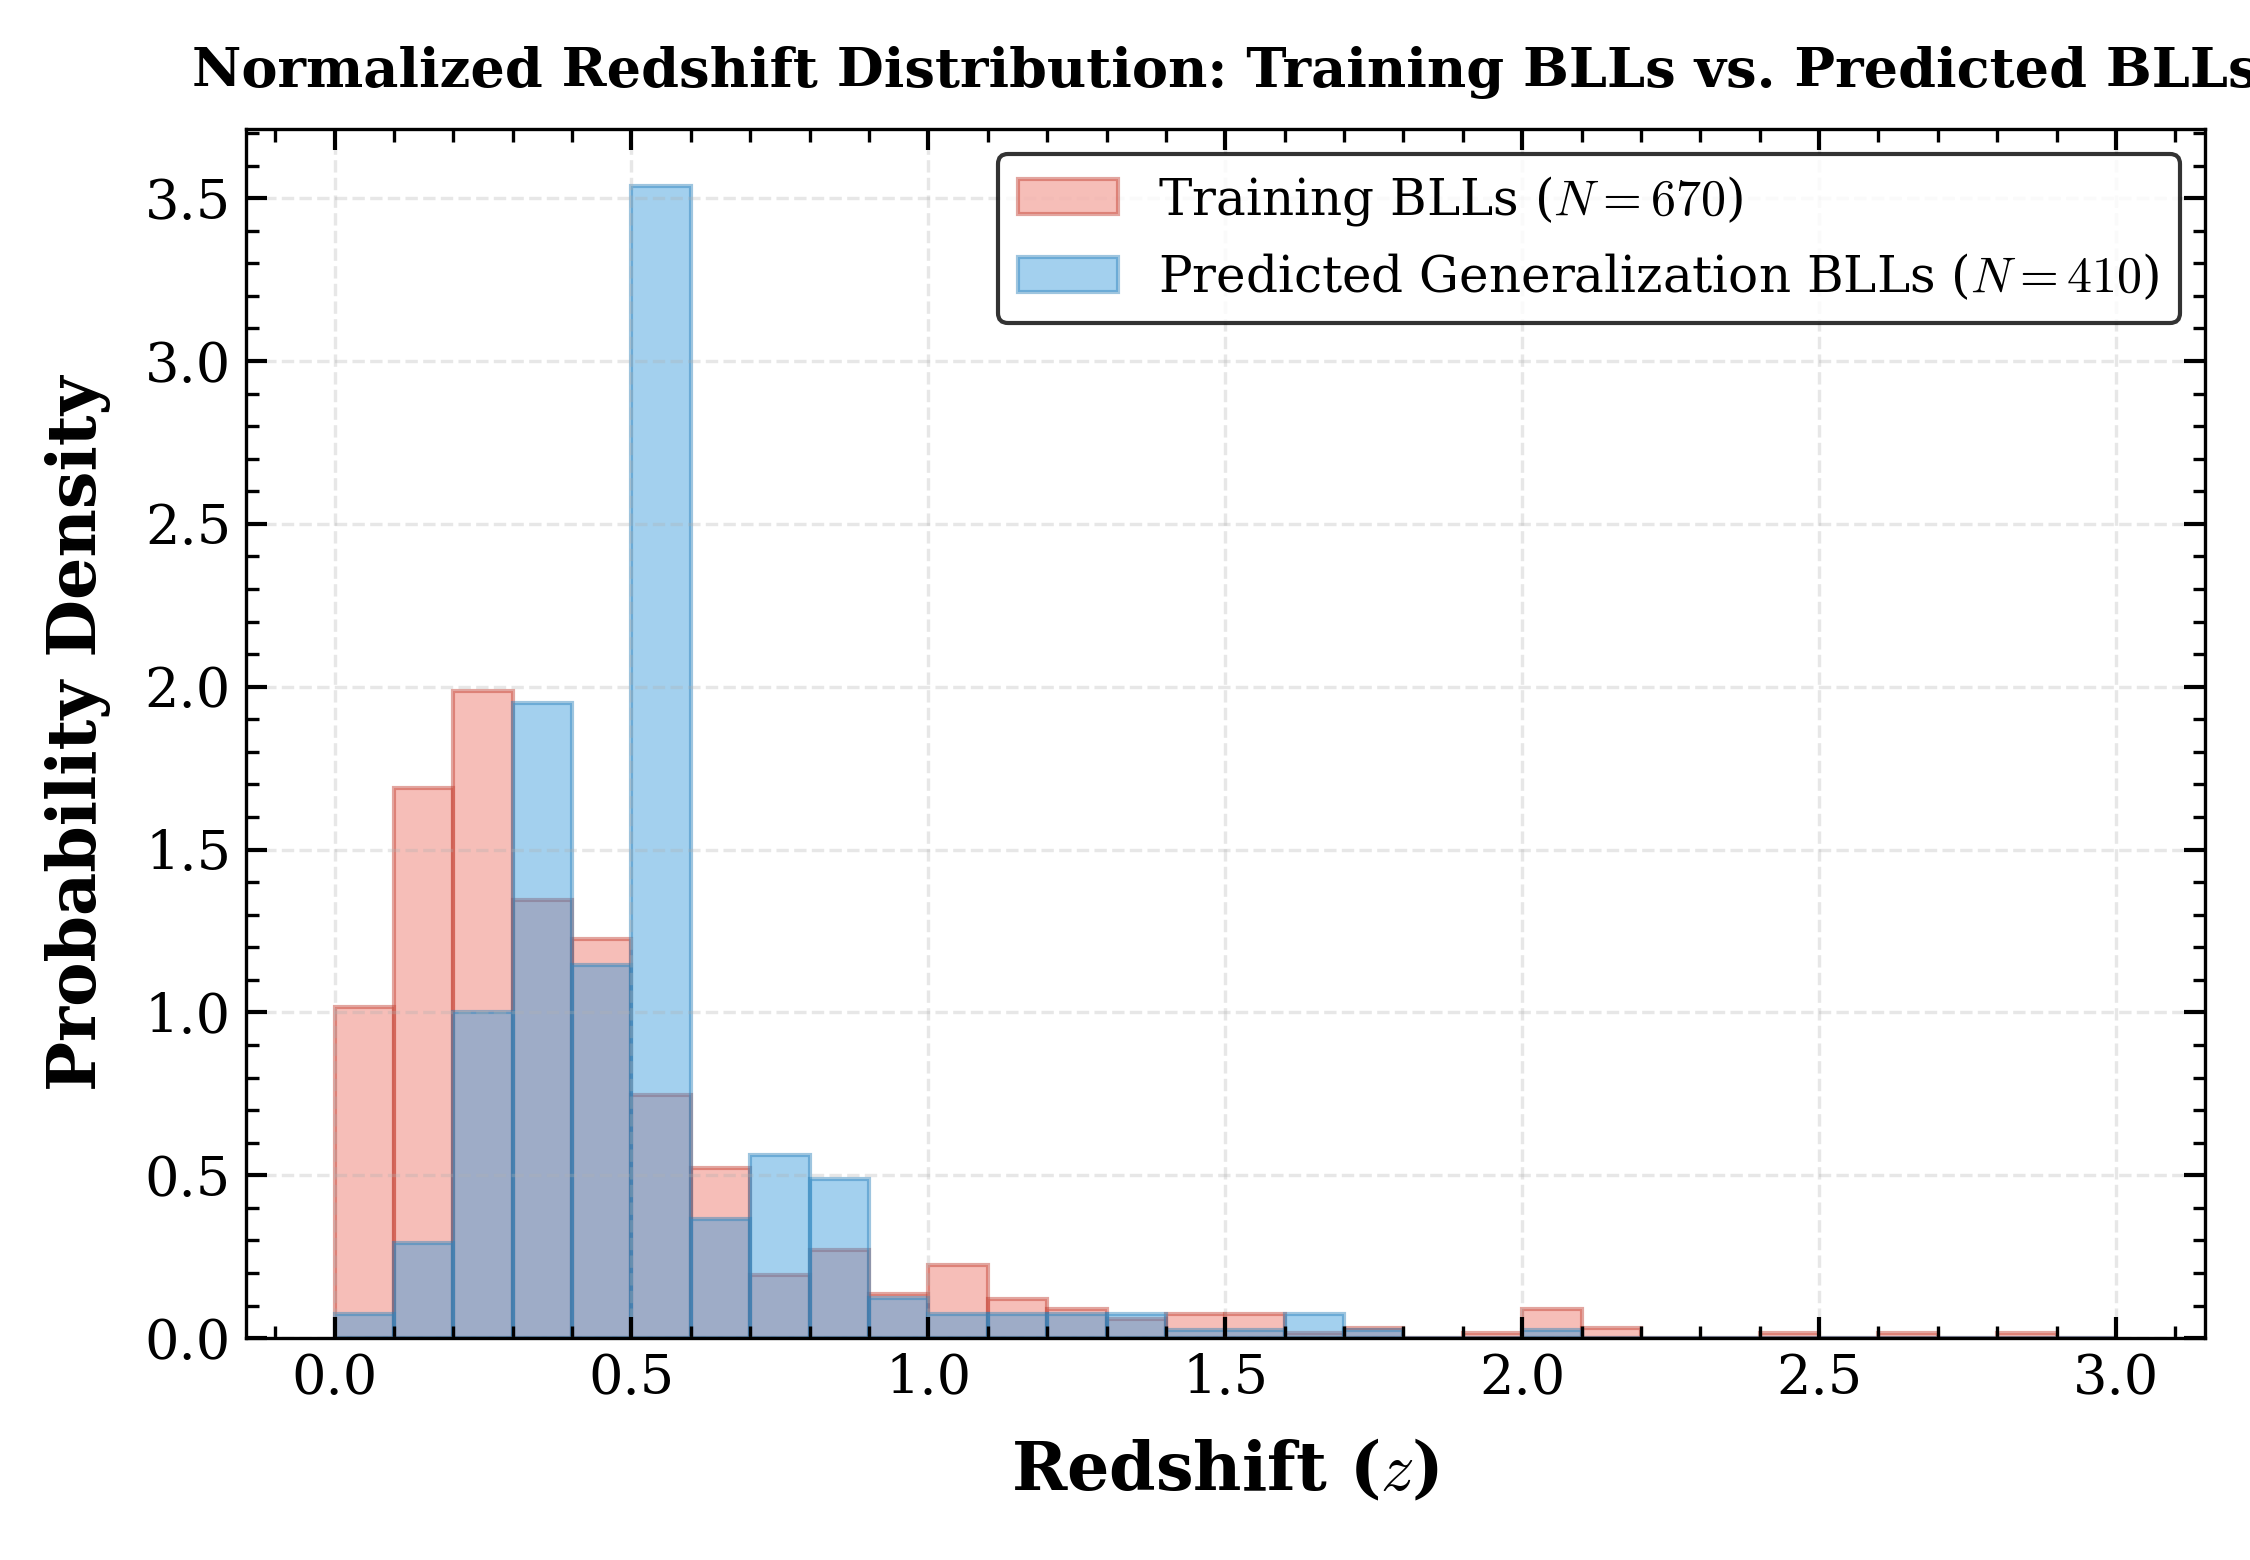
\includegraphics[width=0.82\textwidth,height=0.42\textheight,keepaspectratio]{figures/16_training_vs_generalization_distribution.png}
\caption{Distribution of the redshifts of the training data (red) and the predicted redshifts of the generalization set, from a stacked ensemble trained only on BLLs (turquoise).}
\label{fig:stacked_ensemble_hist_bll}

\vspace{0.6cm}

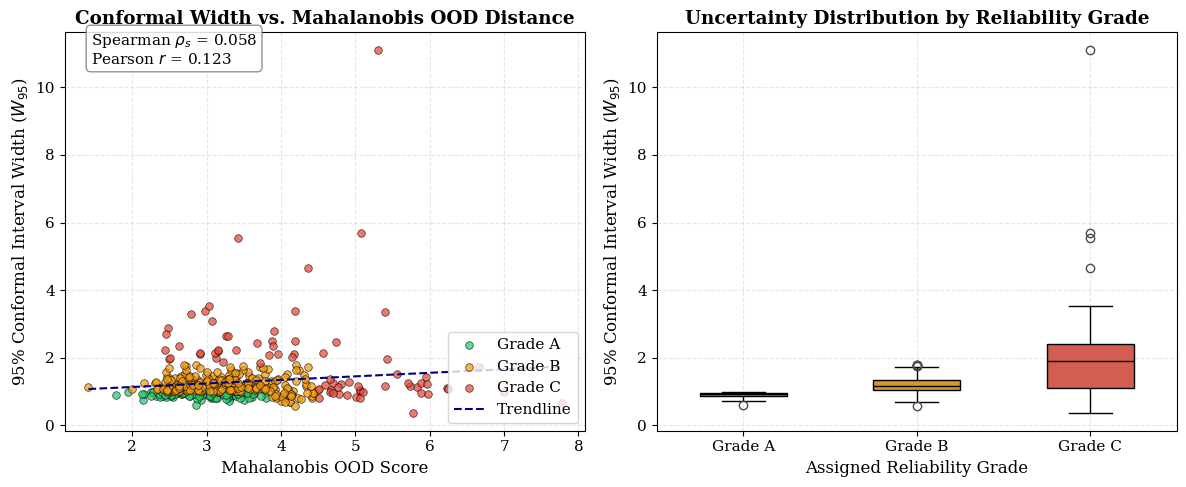
\includegraphics[width=0.96\textwidth,height=0.32\textheight,keepaspectratio]{figures/17_mahalanobis_conformal_relation.png}
\caption{Relationship between high-dimensional feature geometry (Mahalanobis out-of-distribution distance) and predictive uncertainty (95\% conformal prediction interval width) for the 410 range-bounded BLL generalization sources. Left panel: Scatter plot of the 95\% conformal prediction interval width vs.\ the Mahalanobis OOD score. Points are color-coded by their reliability grades (Grade A: green, Grade B: orange, Grade C: red), and the navy dashed line shows the linear regression trendline. Right panel: Boxplot distributions of the 95\% conformal prediction interval width grouped by their reliability grades, illustrating the statistical alignment between geometric extrapolation and predictive uncertainty.}
\label{fig:mahalanobis_conformal}
\end{figure*}





\clearpage
\begin{thebibliography}{}
\setlength{\itemsep}{1.5pt}
\setlength{\parskip}{0pt}
\small
\bibitem[Valen\c{c}a et al.(2026)]{Valenca2026} Valen\c{c}a, R.~R., Nakazono, L., Izbicki, R., et al.\ 2026, arXiv:2608.10280
\bibitem[Abdalla et al.(2025)]{Abdalla2025} Abdalla, E., Abdalla, F.~B., Marins, A., Queiroz, A., Ribeiro, R.~M., \& Souza, A.~S.~C. 2025, MNRAS, 544, 1514
\bibitem[Abdo et al.(2010)]{Abdo2010} Abdo, A.~A., Ackermann, M., Ajello, M., et al.\ 2010, \apj, 715, 429
\bibitem[Abdollahi et al.(2020)]{Abdollahi2020} Abdollahi, S., Acero, F., Ackermann, M., et al.\ 2020, \apjs, 247, 33
\bibitem[Ackermann et al.(2012)]{Ackermann2012} Ackermann, M., Ajello, M., Allafort, A., et al.\ 2012, \apj, 751, 108
\bibitem[Aihara et al.(2011)]{Aihara2011} Aihara, H., Allende Prieto, C., An, D., et al.\ 2011, \apjs, 193, 29
\bibitem[Ajello et al.(2020)]{Ajello2020} Ajello, M., Angioni, R., Axelsson, M., et al.\ 2020, \apj, 892, 105
\bibitem[Angelopoulos \& Bates(2021)]{Angelopoulos2021} Angelopoulos, A. N., \& Bates, S. G. 2021, arXiv preprint arXiv:2107.07511
\bibitem[Arik \& Pfister(2021)]{Arik2021} Arik, S.~O., \& Pfister, T.\ 2021, AAAI, 35, 6679
\bibitem[Barber et al.(2021)]{Barber2021} Barber, R. F., Candes, E. J., Ramdas, A., \& Tibshirani, R. J. 2021, Ann. Statist., 49, 486
\bibitem[Barlow et al.(1972)]{Barlow1972} Barlow, R. E., Bartholomew, D. J., Bremner, J. M., \& Brunk, H. D. 1972, Statistical Inference under Order Restrictions (New York: Wiley)
\bibitem[Blandford et al.(2019)]{Blandford2019} Blandford, R., Meier, D., \& Readhead, A.\ 2019, \araa, 57, 467
\bibitem[Brescia et al.(2019)]{Brescia2019} Brescia, M., Cavuoti, S., Longo, G., et al.\ 2019, \mnras, 489, 663
\bibitem[Breiman(2001)]{Breiman2001} Breiman, L.\ 2001, Mach. Learn., 45, 5
\bibitem[Cavuoti et al.(2014)]{Cavuoti2014} Cavuoti, S., Brescia, M., D'Abrusco, R., et al.\ 2014, \mnras, 442, 2305
\bibitem[Chen \& Guestrin(2016)]{Chen2016} Chen, T., \& Guestrin, C.\ 2016, KDD, 785
\bibitem[Dainotti et al.(2021)]{Dainotti2021} Dainotti, M.~G., Narendra, A., Rinaldi, E., et al.\ 2021, \apjs, 253, 54
\bibitem[Dom{\'\i}nguez et al.(2019)]{Dominguez2019} Dom{\'\i}nguez, A., Primack, J.~R., Bell, E.~F., et al.\ 2019, \apj, 885, 137
\bibitem[Gaia Collaboration(2023)]{Gaia2023} Gaia Collaboration, Vallenari, A., Brown, A.~G.~A., et al.\ 2023, \aap, 674, A1
\bibitem[Geurts et al.(2006)]{Geurts2006} Geurts, P., Ernst, D., \& Wehenkel, L.\ 2006, Mach. Learn., 63, 3
\bibitem[Ghisellini et al.(2011)]{Ghisellini2011} Ghisellini, G., Tavecchio, F., Foschini, L., et al.\ 2011, \mnras, 414, 2674
\bibitem[Gorishniy et al.(2021)]{Gorishniy2021} Gorishniy, Y., Rubachev, V., Khrulkov, V., \& Babenko, A. 2021, NeurIPS, 34, 18932
\bibitem[Gorishniy et al.(2024)]{Gorishniy2024} Gorishniy, Y., Rubachev, V., \& Babenko, A. 2024, arXiv preprint arXiv:2407.01234
\bibitem[Hastie et al.(2009)]{Hastie2009} Hastie, T., Tibshirani, R., \& Friedman, J.\ 2009, The Elements of Statistical Learning (2nd ed.; New York: Springer)
\bibitem[Hollmann et al.(2022)]{Hollmann2022} Hollmann, N., M{\"u}ller, S., \& Hutter, F. 2022, arXiv preprint arXiv:2207.01848
\bibitem[Jones \& Singal(2017)]{Jones2017} Jones, E., \& Singal, J.\ 2017, \aap, 600, A113
\bibitem[Ke et al.(2017)]{Ke2017} Ke, G., Meng, Q., Finley, T., et al.\ 2017, NeurIPS, 30, 3146
\bibitem[MacKay(1992)]{MacKay1992} MacKay, D. J. C. 1992, Neural Comput., 4, 415
\bibitem[Madejski \& Sikora(2016)]{Madejski2016} Madejski, G., \& Sikora, M.\ 2016, \araa, 54, 725
\text{ }
\bibitem[Mahalanobis(1936)]{Mahalanobis1936} Mahalanobis, P.~C.\ 1936, Proc. Natl. Inst. Sci. India, 2, 49
\bibitem[Nakoneczny et al.(2020)]{Nakoneczny2020} Nakoneczny, S.~J., Bilicki, M., Solarz, A., et al.\ 2020, \aap, 640, A105
\bibitem[Narendra et al.(2022)]{Narendra2022} Narendra, A., Gibson, S.~J., Dainotti, M.~G., et al.\ 2022, \apjs, 259, 55
\bibitem[Prokhorenkova et al.(2018)]{Prokhorenkova2018} Prokhorenkova, L., Gusev, G., Vorobev, A., et al.\ 2018, NeurIPS, 31, 6638
\bibitem[Rousseeuw \& van Zomeren(1990)]{Rousseeuw1990} Rousseeuw, P. J., \& van Zomeren, B. C. 1990, J. Am. Stat. Assoc., 85, 633
\bibitem[Rumelhart et al.(1986)]{Rumelhart1986} Rumelhart, D.~E., Hinton, G.~E., \& Williams, R.~J.\ 1986, Nature, 323, 533
\bibitem[Satheesh Sheeba et al.(2025)]{SatheeshSheeba2025} Satheesh Sheeba, S., Assef, R.~J., Anguita, T., et al. 2025, arXiv:2509.13308

\bibitem[Somepalli et al.(2021)]{Somepalli2021} Somepalli, G., Goldblum, M., Salvador, A., et al.\ 2021, arXiv preprint arXiv:2106.01342
\bibitem[Singal(2015)]{Singal2015} Singal, J.\ 2015, \mnras, 454, 115
\bibitem[Tibshirani(1996)]{Tibshirani1996} Tibshirani, R.\ 1996, JRSSB, 58, 267
\bibitem[Tipping(2001)]{Tipping2001} Tipping, M. E. 2001, J. Mach. Learn. Res., 1, 211
\bibitem[Vovk et al.(2005)]{Vovk2005} Vovk, V., Gammerman, A., \& Shafer, G. 2005, Algorithmic Learning in a Random World (New York: Springer)
\bibitem[Wolpert(1992)]{Wolpert1992} Wolpert, D. H. 1992, Neural Netw., 5, 241
\bibitem[Wright et al.(2010)]{Wright2010} Wright, E.~L., Eisenhardt, P.~R.~M., Mainzer, A.~K., et al.\ 2010, \aj, 140, 1868
\bibitem[Yang et al.(2017)]{Yang2017} Yang, M., Jiang, B., \& Zhao, Y.\ 2017, \aj, 154, 18
\bibitem[Zadrozny \& Elkan(2002)]{Zadrozny2002} Zadrozny, B., \& Elkan, C. 2002, KDD, 694




\bibitem[Actis et al.(2011)]{Actis2011} Actis, M., Agnetta, G., Aharonian, F., et al.\ 2011, Experimental Astronomy, 32, 193
\bibitem[Ahnen et al.(2018)]{Ahnen2018} Ahnen, M.~L., Ansoldi, S., Antonelli, L.~A., et al.\ 2018, \apjl, 863, L10
\bibitem[Biteau et al.(2015)]{Biteau2015} Biteau, J., \& Williams, D.~A.\ 2015, \apj, 812, 60
\bibitem[Dom{\'\i}nguez et al.(2011)]{Dominguez2011} Dom{\'\i}nguez, A., Primack, J.~R., Rosario, D.~J., et al.\ 2011, \mnras, 410, 2556
\bibitem[Falomo et al.(2014)]{Falomo2014} Falomo, R., Pian, E., \& Treves, A.\ 2014, \aapr, 22, 73
\bibitem[Gould \& Schr{\'e}der(1967)]{Gould1967} Gould, R.~J., \& Schr{\'e}der, G.~P.\ 1967, Physical Review, 155, 1404
\bibitem[Hollmann et al.(2025)]{Hollmann2025} Hollmann, N., M{\"u}ller, S., Purucker, L., et al.\ 2025, Nature, 637, 792
\bibitem[IceCube Collaboration(2018)]{IceCube2018} IceCube Collaboration, Aartsen, M.~G., Ackermann, M., et al.\ 2018, Science, 361, eaat1378
\bibitem[Ivezi{\'c} et al.(2019)]{Ivezic2019} Ivezi{\'c}, {\v{Z}}., Kahn, S.~M., Tyson, J.~A., et al.\ 2019, \apj, 873, 111
\bibitem[Kuijken et al.(2019)]{Kuijken2019} Kuijken, K., Heymans, C., Dvornik, A., et al.\ 2019, \aap, 625, A2
\bibitem[Urry \& Padovani(1995)]{Urry1995} Urry, C.~M., \& Padovani, P.\ 1995, \pasp, 107, 803
\end{thebibliography}

\end{document}
